% changer fit pour ajustement
% une fois pour toutes on dit super-Terres (exit les super terres et autres orthographes). 


\documentclass[logos,chaptertoc]{bordeaux-thesis}

%########################################################################
% Extensions
%########################################################################

%Text encoding and fonts
\usepackage[utf8]{inputenc}
\usepackage[T1]{fontenc}
%\usepackage{graphicx}

% Command to display names of astronomical objects (only copy the name for the moment, but in case something more usefull might be done, I created a command
\newcommand{\object}[1]{#1}
\newcommand{\mearth}{\unit{M_\oplus}}

\usepackage{listings}

\lstset{%
%Basic Appearance%
  basicstyle=\footnotesize\ttfamily,
  commentstyle=\itshape\color{gray},
  keywordstyle=\color{purple}\bfseries,
  stringstyle=\color{blue}\rmfamily,
%Basic Layout%
  tabsize=4,
  showtabs=false,
  showspaces=false,
  showstringspaces=false,
%Numbering%
  numbers=left,
  stepnumber=1,
  numberstyle=\scriptsize,
  numbersep=5pt,
%Margins%
  xleftmargin=0.02\textwidth,
  xrightmargin=0.02\textwidth,
  breaklines=true,
%Frame%
  frame=leftline,
  framerule=0.5pt,
  rulecolor=\color{purple},
  framexleftmargin=0em,
%Captions, Index, and so on passed as arguments%
  }

%########################################################################
% Title page
%########################################################################

%Thesis author
\author{Christophe \textsc{Cossou}}

%Title for main language (french)
\title{Effet de la structure du disque sur la formation et la migration des planètes}

%Titles for other languages
\title[english]{Effect of the disc structure on planets formation and migration}


%Keywords for main language (french)
\keywords{Formation planétaire, migration, Disques protoplanétaires, Interactions Disque-Planète, Systèmes Planétaires, Simulations numériques}
%Keywords for other languages languages
\keywords[english]{Planets and satellites: formation, Protoplanetary disks, Planet-disk interactions, planetary systems, Methods: numerical}

%Order number of the thesis
\ordernumber{4910}

%Date of defense
\date{28 novembre 2013}
\submityear{2013}

%If some referees are not part of the commission, you can add them in a separate list with \addreferee (optional)
% One can specify the optional title if, for instance, one is also the jury chairman
% EX : \addreferee[Rapporteur et Président du Jury]{Alessandro}{Morbidelli}{Chargé de Recherche, Nice, OCA}
\addreferee[Rapporteur et Président du Jury]{Alessandro}{Morbidelli}{Chargé de Recherche, Nice, OCA}
%\addreferee{Alessandro}{Morbidelli}{Chargé de Recherche, Nice, OCA}
\addreferee{Caroline}{Terquem}{Lecturer, Oxford, University of Oxford}

%You define the commission member list using \addcommissionmember (mandatory) with an optional role (eg: president, supervisor, etc...)
%\addcommissionmember{Président du Jury}{Aaaaa}{Bbbbbbbb}{Astronome, Université Paris VI, LESIA}
\addcommissionmember{Examinateur}{Richard P.}{Nelson}{Professor, Queen Mary, University of London}
\addcommissionmember{Examinateur}{Aurélien}{Crida}{Maître de conférence, Nice, OCA}
\addcommissionmember{Directeur de thèse}{Sean N.}{Raymond}{Chargé de recherche, Université Bordeaux 1, LAB}
\addcommissionmember{Directeur de thèse}{Arnaud}{Pierens}{Maître de conférence, Université Bordeaux 1, LAB}


\makeindex

\newcommand{\MMR}[2]{\mbox{#1:#2}}

% To be used in all the captions of migrations maps, were I only changed one parameter compared to my reference disk
\newcommand{\refdisk}{Tous les autres paramètres sont identiques au disque de référence \protect\refsec{sec:reference_disk}.}

%########################################################################
% Document start
%########################################################################

\begin{document}
%Print title NOW
\maketitle%

%Disable page numbering
\pagestyle{empty}

\cleardoublepage
\null
% \vfill
% \begin{flushright}
% À Marie, faute de prix Nobel.
% \end{flushright}
% \vfill
%TODO dedicate this PhD to marie?
\vfill
\noindent
\includelogo[width=0.2\textwidth]{logo-lab}\hfill
  \begin{minipage}[b]{.75\textwidth}
  \noindent Th\`{e}se pr\'{e}par\'{e}e au\\{\footnotesize
    \textbf{Laboratoire d'Astrophysique de Bordeaux}\\
    Observatoire Aquitain des Sciences de l'Univers (OASU, UMR 5804-LAB)\\
    2, rue de l'observatoire\\
    \numprint{33271} \textsc{Floirac CEDEX}}
  \end{minipage}
\hfill
\cleardoublepage


%########################################################################
% Multilingual abstracts
%########################################################################

%French abstract:
\begin{abstract}
Au delà du système Solaire et de ses planètes, nous avons maintenant un catalogue de quasiment 1000 exoplanètes qui illustrent la grande diversité des planètes et des systèmes qu'il est possible de former. Cette diversité est un défi que les modèles de formation planétaire tentent de relever. La migration de type 1 est un des mécanismes pour y parvenir. En fonction des propriétés du disque protoplanétaire, les planètes peuvent s'approcher ou s'éloigner de leur étoile. La grande variété des modèles de disques protoplanétaires permet d'obtenir une grande variété de systèmes planétaires, en accord avec la grande diversité que nous observons déjà pour l'échantillon limité qui nous est accessible. Grâce à des simulations numériques, j'ai pu montrer qu'au sein d'un même disque, il est possible de former des super-Terres ou des noyaux de planètes géantes selon l'histoire de migration d'une population d'embryons.
\end{abstract}

%Horizontal rule
\noindent\hspace*{0.35\textwidth}\hrulefill\hspace*{0.35\textwidth}\\[-\bigskipamount]

%English abstract:
\begin{abstract}[english]
In addition to the Solar System and its planets, we now have a database of nearly 1000 planets that emphasize the huge diversity of planets and systems that can be formed. This diversity is a challenge for planetary formation models. Type I migration is one of the mechanisms possible to explain this diversity. Depending on disc properties, planets can migrate inward or outward with respect to their host star. The huge parameter space of protoplanetary disc models can form a huge diversity of planetary systems, in agreement with the diversity observed in the nonetheless small sample accessible to us. Thanks to numerical simulations, I showed that within the same disc, it is possible to form super-Earths or giant planet cores, depending on the migration history of an initial population of embryos.
\end{abstract}
%TODO traduire l'abstract français quand il aura été finalisé

%########################################################################
% Acknowledgments
%########################################################################

\pagebreak\strut\newpage

\chapter*{Remerciements}
Cette section étant sans doute la seule que bon nombre de lecteurs parcourront, je vais donc faire ici la conclusion scientifique de ma thèse, point par point, dans un style aussi soporifique que possible, et en latin, juste par méchanceté gratuite, tout en me délectant du rictus qui doit déformer vos visages à cet instant. 

%Je vous ferai grâce des non remerciements de thèse, parait que ce n'est pas très protocolaire.

%TODO directeur, jury etc

%TODO autres contributeurs, dont franckH

%TODO paragraphe spécial franckS

%TODO les copains, et romuald en particulier, sergi, audrey, émeline

%TODO postérité de quelques clins d'oeil qui ne seront compris que par les personnes concernées, sans éveiller la curiosité des autres. en particulier un truc pour la bretagne, ou tout/tous ou des trucs comme ça.

%TODO remercier macOS et autre trucs à la con

%TODO famille en dernier


\newpage

%########################################################################
% Contents
%########################################################################

\strut\newpage

\tableofcontents
\mtcaddchapter % To have correct minitocs

% List of figures and tables must be right after the table of contents
\listoffigures
\mtcaddchapter % To have correct minitocs

\listoftables
\mtcaddchapter % To have correct minitocs

\newpage

%########################################################################
% Introduction
%########################################################################

%Enable page numbering
\pagestyle{fancy}

\chapter*{Introduction}
\addstarredchapter{Introduction}% To be used instead of addcontentsline in order to have the good minitoc. If not, the starred chapter create a shift in the minitocs.

%TODO parler de formation planétaire (en citant des papiers, sans rentrer dans les détails. notamment pollack, alibert)

%TODO une des grandes questions c'est  : comment on forme des noyaux de jupiter et Kepler 11?

%TODO voir l'intro de franckH et en particulier la partie sur laplace et descartes?

La pluralité des mondes est un concept qui a lentement évolué au cours des âges. Dans l'antiquité grecque l'univers fini, sphérique et géocentrique d'Aristote (384--322 av. JC) s'oppose à l'univers infini et discontinu des atomistes. Pour Epicure (v 342--270 av JC), il existe une pluralité de \textit{kosmoi}, portions de ciels contenant les corps célestes. Thales (v 625-547 av. JC) pense que d'autres astres pourraient être similaires à la Terre. 

Le débat de la vie ailleurs et de l'existence d'autres planètes autour d'autres étoiles a animé la communauté scientifique
depuis l'antiquité. Souvent influencé par les convictions religieuses et les modèles du système solaire en vigueur, il était
parfois même dangereux d'émettre l'hypothèse que d'autres planètes ou d'autres formes de vies puissent exister, l'idée de la
pluralité des civilisations étant indissociable de la question de la pluralité des mondes physiques. 

\begin{quote}
\og mesmes n'y auroit-il pas de l'apparence à croire que chaque globe est un monde, \& que tout autant qu'ils sont ce sont autant de mondes, comme autant de fiefs qui relevent de l'Empire Divin, \& eternel, assis dans la vaste estenduë du Ciel etherée, par le moyen duquel estans liez, comme par un lien commun, ils demeurent suspendus, \& que la vaste estenduë de l'Univers est composée de toutes ces differentes natures?\fg 

--- Jean d'Espagnet, \textit{La Philosophie naturelle restablie en sa pureté}, 1651, p. 241 \cite{espagnet1651philosophie}
\end{quote}

Ces questions ont longtemps été des expériences de pensées, plus philosophiques et métaphysiques qu'étayées par de quelconques observations. La découverte progressive du système solaire et de la diversité des planètes qui la compose a permis de situer la Terre dans un contexte un peu plus large. La question de la formation des planètes s'est alors posée. Remarquant la quasi coplanarité des orbites du système Solaire, Kant (1755) puis Laplace (1796) ont introduit le concept de nébuleuse solaire primitive, disque de matière duquel les planètes étaient issues. 

La ligne des glaces, séparation imaginaire au delà de laquelle l'eau est sous forme solide, s'intégrait bien dans ce concept et dans le cas du système Solaire. Pas beaucoup de matière en dessous de la ligne des glaces, nous formons des planètes essentiellement rocheuses, peu massives. Au delà, la quantité de matière augmente, nous formons des géantes gazeuses. Durant leur formation, les planètes n'évoluent pas beaucoup. La Nébuleuse Solaire de Masse Minimale (MMSN) a ainsi été inventée. Elle représente le disque le moins moins massif qui est nécessaire pour former les planètes du système Solaire. Pour cela, la masse de chaque planète est répartie sur un anneau de matière afin de remplir tout l'espace interplanétaire par de la matière. Cette masse est corrigée pour tenir compte du gaz (abondant dans le cas de géantes comme Jupiter, mais rare pour une planète comme la Terre). On obtient donc un profil de densité de surface en loi de puissance $\Sigma(R)=1700 * R^{-\sfrac32}$ \citep{
weidenschilling1977distribution, hayashi1981structure}.

La découverte de la première exoplanète\footnote{Planète orbitant autour d'une étoile autre que notre Soleil.} \citep{wolszczan1992planetary} a quelque peu bouleversé le cadre théorique de la formation planétaire.

Bien que cette dernière fut découverte en 1992, c'est en 1995 avec \object{51 Peg b} \citep{mayor1995jupiter} que la chasse aux exoplanètes a véritablement commencé. Cette planète a ceci de particulier qu'elle est semblable à Jupiter, mais plus proche de son étoile que ne l'est Mercure dans notre système. Elle orbite son étoile en $4.2$ jours. Le modèle alors en vigueur pour former les planètes était mis en défaut. Aucun modèle ne permettait de former une telle planète. 

Des travaux théoriques ont alors montré que la migration planétaire via interaction de la planète avec le disque de gaz pouvait expliquer la présence d'une géante gazeuse très proche de son étoile. Cette idée de la migration planétaire a depuis été raffinée et a même permis d'élaborer de nouvelles hypothèses sur la formation et l'évolution du système solaire. En particulier le modèle du \og grand Tack\fg \citep{morbidelli2007dynamics, pierens2011twophase}, dans lequel Jupiter et Saturne migrent séparément vers l'intérieur, sont capturés en résonance puis migrent de concert vers l'extérieur, pouvant expliquer par la même occasion la masse étonnamment petite de Mars \citep{walsh2011low}. 

Depuis, multipliant les campagnes d'observations, les missions dédiées et les techniques de détection, on arrive, 20 ans après la première découverte à un catalogue d'exoplanètes toujours plus fourni, montrant une population extrêmement riche et variée. 939 exoplanètes ont été à ce jour observées (14 août ; \url{http://exoplanet.eu/}), apportant toujours plus de contraintes aux modèles de formation planétaire. 

Compte tenu de la difficulté à détecter les exoplanètes en raison de leur faible masse et luminosité, un premier constat s'impose : ce ne sont pas des objets rares. Si auparavant on pouvait encore en douter, il ne fait aujourd'hui plus aucun doute que les planètes sont des objets communs. C'est d'autant plus flagrant quand on note que la grande majorité des exoplanètes détectées l'ont été autour d'étoiles à moins de 400 pc du Soleil comme illustré dans \reffig{fig:milky_way_exoplanet}. 

\begin{figure}[htb]
\centering
\includegraphics[width=0.45\linewidth]{figure/milky_way_exoplanets.pdf}
\caption{Image de la voie lactée avec indication de la position approximative du système solaire ainsi que de la zone (en noir) contenant la majorité des exoplanètes détectées à ce jour.}\label{fig:milky_way_exoplanet}
\end{figure}


En multipliant les méthodes de détections et les instruments, et surtout en ayant de plus en plus de planètes, il devient possible d'estimer la probabilité pour qu'une étoile héberge au moins une planète \citep{mayor2011road}. D'autres études estiment même la sensibilité de cette fréquence d'occurrence en fonction de paramètres stellaires \citep{fischer2005planet, johnson2007new, howard2012occurrence} ou planétaires \citep{mayor2011road, howard2010occurrence}. 

Mais le point qui me semble le plus intéressant est la découverte de types de planètes qui n'existent pas dans le système solaire. En un mot : diversité. Que ce soient les Jupiters chauds, comme \object{51 Peg b} ou les super-Terres comme \object{Gliese 1214 b}, ces planètes n'ont pas d'équivalent dans le système solaire. Ces variétés de composition, de taille, de systèmes nous offrent un champ de connaissance toujours plus grand dans lequel tester nos modèles de formations planétaire. Ils nous permettent aussi de mieux comprendre notre propre système, comment il s'est formé, et surtout de le mettre en perspective par rapport à tous les autres systèmes planétaires que nous observons maintenant.

Ma thèse s'inscrit dans ce cadre toujours changeant, où de nouvelles planètes viennent sans cesse remettre en cause les modèles de formation. Un type particulier de planète aura aiguisé mon intérêt en particulier, ce sont les super-Terres ($1$ - $10\mearth$). Déjà parce qu'elles sont rocheuses, à la fois semblables et différentes de la Terre, mais aussi et surtout parce qu'il n'en existe pas dans le système Solaire. Mon but a donc été d'imaginer des modèles dans lesquels la formation du système Solaire et des super-Terres serait compatible, au sein d'un même cadre théorique.

Dans un premier chapitre \refsec{sec:chap1}, je vais présenter la physique des disques, à la fois la formation et l'évolution d'un disque protoplanétaire, mais aussi les interactions entre ce dernier et les planètes qui se forment en son sein. Ensuite, je présenterai les modèles numériques que j'ai utilisé \refsec{sec:chap2}. Puis je détaillerai la migration planétaire dans une grande variété de disques protoplanétaires \refsec{sec:chap3}, variant divers paramètres clés afin d'en étudier l'influence sur la migration. Je présenterai des mécanismes de formation planétaire \refsec{sec:chap4}, en portant une attention particulière aux super-Terres. Enfin je conclurai en récapitulant les résultats principaux de ma thèse et les perspectives qui en découlent \refsec{sec:discussion}.

%TODO HERE

\chapter{Formation Planétaire}\label{sec:chap1}
 \section{Les disques protoplanétaires}
%TODO voir thèse mordasini, et les articles de mordasini, alibert, ida et lin, histoire de voir ce qu'ils font)


\subsection{Formation et évolution}
Les planètes se forment à partir d'un disque protoplanétaire constitué de gaz et de poussière. On observe de tels disques autour d'étoiles jeunes, essentiellement pendant les premiers millions d'années de leur existence. Il peut sembler étrange de voir que les disques d'accrétion sont aussi courants dans l'univers et surtout de voir qu'il apparaît spontanément un axe de rotation. 

\begin{figure}[htb]
\centering
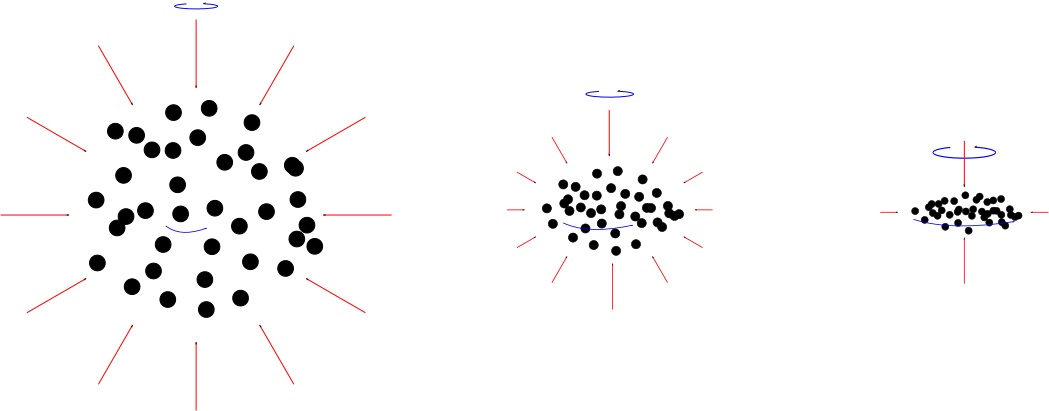
\includegraphics[width=0.8\linewidth]{figure/disk_collapse.pdf}
\caption{Schéma de l'effondrement d'un nuage moléculaire, représenté par un amas épars de cellules de gaz représentées par des points noirs.}\label{fig:disk_collapse}
\end{figure}

\reffig*{fig:disk_collapse} montre le principe de l'effondrement gravitationnel d'un nuage. Loin de moi l'idée de comparer les patineuses avec un nuage de gaz mais pour illustrer l'effondrement gravitationnel d'un nuage moléculaire, rien de mieux que le patinage artistique. 

Quand une patineuse tourne sur elle même, vous observerez qu'en ramenant les bras le long du corps, sa rotation s'accélère. À l'inverse, sa rotation diminue quand elle écarte les bras. C'est une illustration de la conservation du moment angulaire. 

Pour un nuage moléculaire c'est exactement pareil. À mesure que le nuage s'effondre sur lui même, et afin de satisfaire à la conservation du moment angulaire, ce dernier voit sa rotation accélérer. C'est ainsi que le disque d'accrétion, résultat de l'effondrement du nuage de gaz, est en rotation. L'effondrement d'un nuage moléculaire étant beaucoup plus violent que le fait de ramener ses bras le long de son corps, l'accélération de la rotation est elle aussi beaucoup plus drastique dans le cas du nuage. 

Initialement, il est hautement improbable que le moment angulaire du nuage soit parfaitement nul. C'est ainsi que même si sa rotation est imperceptible lors des premiers stades de son effondrement gravitationnel, le disque d'accrétion fini toujours en rotation. 

%\bigskip
%
%L'évolution de tels objets au cours du temps est un sujet de recherche actif, mais le principe de base est que lors de l'effondrement gravitationnel d'un nuage moléculaire diffus, le gigantesque moment angulaire de cette masse ne peut s'évacuer instantanément. 
%
%La quantité totale de moment angulaire doit être conservée. En conséquence, soit deux cellules de gaz vont échanger du moment angulaire par friction (celle qui gagne du moment angulaire migre vers l'extérieur, l'autre migrant vers l'intérieur), soit du moment angulaire est perdu soit par accrétion d'une particule de gaz sur l'étoile, soit par évaporation du gaz sur les bords du disque.
%
%Mais ces processus prennent du temps, beaucoup plus de temps que n'en met le gaz pour faire une orbite autour de l'étoile. De l'ordre du million d'années. C'est durant ce labs de temps que les planètes se forment. Le processus est complexe et très loin d'être compris. Il est cependant clair que les interactions entre le disque de gaz et les planètes ont un rôle prépondérant dans la formation d'un système stellaire, que ce soit pour les planètes géantes, dont on pense qu'elles ont accrété une partie du gaz du disque pour en faire leur enveloppe, ou les planètes telluriques, beaucoup plus denses, principalement composées des poussières du disque.
%
%\bigskip
%
%Afin de décrire la physique des disques, on a besoin principalement de deux équations. L'équation de Navier-Stokes pour décrire le comportement fluide du disque de gaz et l'équation de conservation de l'énergie, pour décrire la température du disque.

Pour décrire correctement un disque de gaz, il est nécessaire de définir les trois équations suivantes : 
\begin{itemize}
\item L'\textbf{équation de continuité} ou par équivalence la conservation de la masse du disque.
\begin{align}
r\dpd{\Sigma}{t} + \dpd{}{r}\left(r\Sigma(r)v_r\right) &= 0\label{eq:disk_continuite}
\end{align}
où $r$ est la distance à l'étoile centrale, $\Sigma$ est le densité de surface du disque et $v_r$ la vitesse radiale à une distance donnée.
\item L'\textbf{équation de conservation de l'énergie}. Ceci permet de calculer la température en tout point du disque à partir des phénomènes physiques que l'on souhaite décrire
\begin{align}
\label{eq:disk_energy}
\end{align}
\item L'\textbf{équation de conservation du moment angulaire}. Cette dernière décrit l'évolution fluide du disque
\begin{align}
r\dpd{}{t}\left(\Sigma r^2 \Omega\right) + \dpd{}{r}\left(r \Sigma v_r \cdot r^2 \Omega\right) &= \inv{2\pi} \dpd{}{r} \left(2\pi r \cdot \nu \Sigma A \cdot R\right)\label{eq:disk_angular_momentum}
\end{align}
\end{itemize}

\subsection{Modélisation de l'évolution hydrodynamique du disque}
Avant de considérer l'évolution d'un disque, il est important de regarder sa masse par rapport à la masse de l'étoile centrale. En effet, si la masse du disque est de l'ordre de la masse de l'étoile, alors des instabilités se développent et on ne peut plus négliger l'autogravité du disque. 

Le \gras{paramètre de Toomre} $Q$, défini par :
\begin{align}
Q &= \frac{\kappa {c_{s}}^2}{\pi G \Sigma}
\end{align}\index{$Q$}
est un indicateur de la stabilité du disque par rapport à l'autogravité.

La densité de surface $\Sigma$\index{$\Sigma$} mesure l'importance de l'\gras{auto-gravité}. La vitesse du son $c_{s}$ est liée à la pression thermique ; la \gras[fréquence!epicyclique@épicyclique]{fréquence épicyclique} $\kappa$ détermine quant à elle la force du cisaillement dans le disque.

\bigskip

Si $Q<1$ alors le gaz est instable gravitationnellement et il commence à s'effondrer sur lui même et former des \og tas\fg de matière.
Si $Q>1$, le disque est stable.

%\begin{remarque}
%Dans les disques protoplanétaires, $Q\gg 1$ ce qui implique que leur auto-gravité n'est pas importante \citep{masset2008planet}.
%\end{remarque}

Nous ne considérerons que des disques dont la masse $M_\text{d}$ est faible devant la masse de l'étoile $M_\star$ :
\begin{align}
\frac{M_\text{d}}{M_\star} &\lesssim 0.1
\end{align}
Si tel n'était pas le cas, le temps pour que le disque perde suffisamment de masse pour se retrouver dans le cas qui nous intéresse sera court devant la vie du disque et le temps de formation planétaire. Étant donné qu'on ne s'intéresse qu'aux derniers stades de la formation planétaire, à savoir quand les embryons planétaires ont une masse de l'ordre du dixième de masse terrestre au minimum, il est raisonnable de penser que le disque sera dans un stade peu dense où l'approximation $Q>1$ sera valable.

Dans un tel cas, c'est le potentiel gravitationnel de l'étoile qui domine la dynamique du gaz. En négligeant l'effet de la pression de ce dernier, on peut donc écrire la vitesse angulaire du gaz comme étant égale à la vitesse angulaire képlerienne : 
\begin{align}
\Omega &= \sqrt{\frac{GM_\star}{r^3}}
\end{align}
où $G$ est la constante de gravitation, et $r$ la distance à l'étoile. Dans la pratique, il est à noter que la vitesse est légèrement sous-képlerienne. 

\bigskip

À l'instar des planètes du système solaire qui orbitent autour du Soleil d'autant plus vite qu'elle sont proche de ce dernier, les éléments fluides du disques de gaz vont orbiter beaucoup plus vite au bord interne qu'ils ne le font au bord externe. Il existe donc une force de cisaillement entre deux anneaux de gaz concentriques, dûs à leur différence de vitesse. Cette différence de vitesse génère des frottements à cause de la viscosité du disque $\nu$ (dont nous parlerons plus en détail plus loin \refsec{sec:viscosite}) qui chauffe le gaz en lui faisant perdre de l'énergie. En conséquence, une partie de l'énergie gravitationnelle du gaz est convertie en chaleur, qui est ensuite évacuée par le rayonnement de corps noir du gaz. 

\bigskip

La première conséquence est qu'un terme visqueux va apparaître dans l'équation de l'énergie, comme nous le verrons par la suite. 

La deuxième conséquence, c'est que le gaz perds de l'énergie, et donc dérive lentement vers l'étoile centrale qui accrète petit à petit le gaz du disque. 

On définit donc une vitesse de dérive négative $v_r$, orientée vers l'étoile, qui entraine petit à petit le gaz du disque.

\bigskip

On cherche maintenant à faire un bilan de moment cinétique pour un anneau de gaz compris entre les rayons $R$ et $R+\Delta R$, avec $\Delta R \ll R$ \reffig{fig:disk_ring}. Le moment cinétique $\vect{J}$ d'une particule de masse $m$ est défini par :
\begin{align}
\vect{J} &= \vect{r} \wedge (m\vect{v})
\end{align}
où $\vect{r}$ et $\vect{v}$ sont respectivement la position et la vitesse de la particule.

\bigskip

\begin{figure}[htb]
\centering
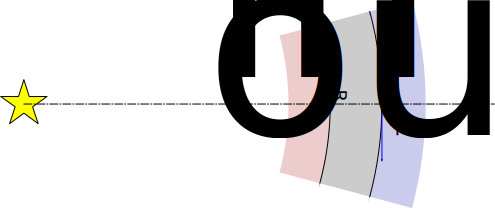
\includegraphics[width=0.7\linewidth]{figure/disk_ring.pdf}
\caption{Représentation d'un anneau de largeur $\Delta r$ et du bilan de moment angulaire de ce dernier.}\label{fig:disk_ring}
\end{figure}

On cherche dans un premier temps à faire le bilan de masse de l'anneau considéré. Sa masse s'écrit :
\begin{align}
m_a &= 2\pi R \Delta R \Sigma(R)\label{eq:m_a}
\end{align}

\bigskip

Soit $-v_r\hat{e}_r$ la vitesse radiale du gaz. Cette vitesse est responsable d'un certain taux d'accrétion du gaz du disque sur l'étoile centrale. On cherche maintenant à modéliser cette accrétion pour le bilan de moment cinétique sur l'anneau.

Pour cela, on cherche à exprimer la variation de masse de l'anneau, ainsi que le moment cinétique emporté par cette variation de masse. 

Au bord interne $R$, par unité de temps, la masse entrant ou sortant de l'anneau est :
\begin{align}
\dif M(R) &= 2\pi R \cdot -v_r(R) * \Sigma(R)
\end{align}
En effet, en multipliant la circonférence de l'anneau par la vitesse, on obtient une sorte de surface par unité de temps qui représente ce qui sort de la frontière virtuelle représentée par l'anneau en $r=R$. Si la vitesse est positive (négative), alors de la masse rentre (sort) dans l'anneau. 

De même on a : 
\begin{align}
\dif M(R+\Delta R) &= 2\pi (R+\Delta R) \cdot -v_r(R+\Delta R) * \Sigma(R+\Delta R)
\end{align}

La conservation de la masse implique alors que la dérivée temporelle de la masse de l'anneau est égale à la masse qui entre ou sort de ses frontières. On a ainsi : 
\begin{align*}
\dpd{}{t}\left(\cancel{2\pi} R \Delta R \Sigma(R)\right) &= \cancel{2\pi} (R+\Delta R) \cdot -v_r(R+\Delta R) * \Sigma(R+\Delta R) - \cancel{2\pi} R \cdot -v_r(R) * \Sigma(R)\\
\dpd{}{t}\left(R \Delta R \Sigma(R)\right) &= - (R+\Delta R) \cdot v_r(R+\Delta R) * \Sigma(R+\Delta R) +  R \cdot v_r(R) * \Sigma(R)
\end{align*}

$R$ et $\Delta R$ sont des variables indépendantes du temps. On peut donc les sortir de la dérivée partielle en fonction du temps. 

En faisant passer le terme $\Delta R$ dans le second membre de l'équation, on fait apparaître des termes de la forme 
\begin{align*}
\frac{U(R+\Delta R) - U(R)}{\Delta R}
\end{align*}

En faisant tendre l'épaisseur $\Delta R$ de l'anneau vers 0, on fait ainsi apparaitre une forme différentielle : 
\begin{align*}
\lim_{\Delta R \rightarrow 0} \frac{U(R+\Delta R) - U(R)}{\Delta R} &= \dpd{U}{r}(R)
\end{align*}

On obtient alors :
\begin{important}
\begin{align}
R\dpd{\Sigma}{t} + \inv{R}\dpd{}{r}\left(R v_r \Sigma\right)\label{eq:conservation_masse}
\end{align}
\end{important}

\bigskip

On cherche maintenant à faire le bilan de moment cinétique de ce même anneau. Son moment cinétique est défini par :
\begin{align}
\vect{J_a} &= \vect{R} \wedge (m_a\vect{v(R)}) \nonumber\\
&= m_a \cdot R \cdot R\Omega(R)\nonumber\\
&= 2\pi R \Delta R \Sigma(R)\cdot R \cdot R\Omega(R)\nonumber\\
\vect{J_a} &= 2\pi R^3 \Delta R \Sigma(R)\Omega(R)\label{eq:J_a}
\end{align}
où $\Sigma$ et $\Omega$ sont la densité de surface et la vitesse angulaire du gaz à la position $R$ dans le disque.

La quantité de moment cinétique de ces masses là est respectivement :
\begin{subequations}
\begin{align}
\dif J(R) &= \vect{r} \wedge \left(\dif M(R) \vect{v}(R)\right)\nonumber\\
\dif J(R) &= \dif M(R) \cdot R^2\Omega(R)\hat{e}_z\label{eq:dJ_in}\\
\dif J(R+\Delta R) &= \vect{r} \wedge \left(\dif M(R+\Delta R) \vect{v}(R+\Delta R)\right)\nonumber\\
\dif J(R+\Delta R) &= \dif M(R+\Delta R) \cdot \left(R+\Delta R\right)^2\Omega(R+\Delta R)\hat{e}_z\label{eq:dJ_out}
\end{align}\label{eq:dJ}
\end{subequations}

\bigskip

À ceci s'ajoute la variation de moment cinétique induite par la friction entre anneaux concentriques, en d'autres termes, dus à la viscosité du disque. Cette variation de moment cinétique est représentée sous la forme d'un couple exercé par les anneaux internes et externes à celui considéré. 

Le taux de cisaillement $A$ est donné par : 
\begin{align}
A &= r \dod{\Omega}{r}
\end{align}
et est une illustration de la viscosité d'un fluide. Plus le fluide est visqueux, et moins le cisaillement est important. C'est à dire que plus un fluide est visqueux, et plus son comportement se rapproche de celui d'un solide. En conséquence, par frottement, les éléments fluides sont agglomérés, et le gradient de vitesse est très faible, le cisaillement l'est aussi par extension. 

La force visqueuse par unité de longueur est définie par :
\begin{align}
\dif F_\text{vis} &= \nu \Sigma A = \nu \Sigma r \dod{\Omega}{r}
\end{align}

La force visqueuse induite par les anneaux entourant l'anneau considéré est alors : 
\begin{subequations}
\begin{align}
\vect{F_\text{in}}(R) &= 2\pi R * \dif F_\text{vis}(R) = 2\pi\nu \Sigma R^2 \dod{\Omega}{r}(R) \hat{e}_\theta\\
\vect{F_\text{out}}(R+\Delta R) &= 2\pi (R+\Delta R) * \dif F_\text{vis}(R+\Delta R) = 2\pi\nu \Sigma (R+\Delta R)^2 \dod{\Omega}{r}(R+\Delta R) \cdot \hat{e}_\theta
\end{align}
\end{subequations}
L'anneau interne tournant plus vite, la force est dirigée dans le sens de rotation $\hat{e}_\theta$. À l'inverse, l'anneau externe tourne moins vite, il tend à freiner l'anneau de référence et s'oppose à son mouvement. La force est donc opposée au sens de rotation.

\bigskip

Ainsi, le couple $\vect{\Gamma}=\vect{r}\wedge\vect{F}$ issu de chacun des anneaux entourant celui de référence s'écrit :
\begin{subequations}
\begin{align}
\vect{\Gamma_\text{in}} &= R\hat{e}_r\wedge\vect{F_\text{in}}\nonumber\\
\vect{\Gamma_\text{in}} &= 2\pi\nu \Sigma R^3 \dod{\Omega}{r}(R) \hat{e}_z\label{eq:G_in}\\
\vect{\Gamma_\text{out}} &= (R+\Delta R)\hat{e}_r\wedge\vect{F_\text{out}}\nonumber\\
\vect{\Gamma_\text{out}} &= 2\pi\nu \Sigma (R+\Delta R)^3 \dod{\Omega}{r}(R+\Delta R) \hat{e}_z\label{eq:G_out}
\end{align}\label{eq:J_torques}
\end{subequations}

\bigskip

On fait maintenant un bilan des variations de moment angulaire pour l'anneau de gaz. Pour celà on dit que la variation de moment angulaire (que l'on écrit en dérivant $J_a(t)$) est égale à la différence de moment angulaire entre $R+\Delta R$ et $R$ à laquelle s'ajoute la différence entre les deux couples visqueux qui s'appliquent au bord externe et interne. Ce qui donne : 
\begin{align}
\dod{J_a}{t} &= \dif J(R+\Delta R) - \dif J(R) + \Gamma_\text{out} - \Gamma_\text{in}\label{eq:cons_J_a}
\end{align}

En utilisant \refeq{eq:J_a}, \refeq{eq:dJ}, \refeq{eq:J_torques}, dans \refeq{eq:cons_J_a}
\begin{align*}
\begin{split}
\dpd{}{t}\left(2\pi R^3 \Delta R \Sigma(R)\Omega(R)\right) &= -\left[\left(R+\Delta R\right)^3v_R(R+\Delta R) \Sigma(R+\Delta R) \Omega(R+\Delta R)\right.\\
&\left. - R^3 v_R(R) \Sigma(R) \Omega(R)\right] + \left[\nu(R+\Delta R)^3\Sigma(R+\Delta R)\right.\\
&\left. \dod{\Omega}{r}(R+\Delta R)-\nu \Sigma(R) R^3 \dod{\Omega}{r}(R)\right]
\end{split}
\end{align*}



On fait tendre $\Delta R$ vers 0, et de manière similaire au bilan de masse obtenu précédemment, il vient alors 
\begin{align*}
\dpd{}{t}\left(R^3 \Sigma\Omega\right) &= -\dpd{}{r}\left(R^3 v_R \Sigma \Omega\right) + \dpd{}{r}\left(\nu \Sigma R^3 \dod{\Omega}{r}\right)\\
\intertext{$R$ et $t$ sont des variables indépendantes, on peut donc sortir $R$ de la dérivée partielle temporelle afin de faire apparaître une forme qui fait penser à une équation de continuité.}
R\dpd{}{t}\left(R^2 \Sigma\Omega\right) &= -\dpd{}{r}\left(R^3 v_R \Sigma \Omega\right) + \dpd{}{r}\left(\nu \Sigma R^3 \dod{\Omega}{r}\right)
\end{align*}

$R$ et $t$ étant des variables indépendantes, on peut écrire :
\begin{align}
R\dpd{}{t}\left(\Sigma R^2\Omega\right) + \dpd{}{r}\left(R^3 v_R \Sigma \Omega\right) &= \dpd{}{r}\left(\nu \Sigma R^3 \dod{\Omega}{r}\right)\label{eq:ang_mom_01}
\end{align}

\bigskip

On suppose que $\dpd{\Omega}{t}=0$ vu que le potentiel gravitationnel est indépendant du temps (on ne considère pas une masse variable de l'étoile due à l'accrétion), et sachant que $R$ ne dépend pas explicitement de $t$, en utilisant la formule : 
\begin{align*}
\dpd{uv}{x} &= \dpd{u}{x}v + u\dpd{v}{x}
\end{align*}
on peut écrire :
\begin{align}
\dpd{}{t}\left(\Sigma\cdot R^2\Omega\right) &= \left(R^2\Omega\right)\dpd{\Sigma}{t} + \Sigma\cancelto{0}{\dpd{R^2\Omega}{t}}\label{eq:ang_mom_tmp_01}
\end{align}

De même : 
\begin{align}
\dpd{}{r}\left(R^3 v_R \Sigma \Omega\right) &= \dpd{}{r}\left(R v_R \Sigma \cdot R^2\Omega\right)\nonumber\\
&= \left(R^2\Omega\right)\dpd{}{r}\left(R v_R \Sigma\right) + R \Sigma v_R \dpd{}{r}\left(R^2\Omega\right)\label{eq:ang_mom_tmp_02}
\end{align}

En utilisant \refeq{eq:ang_mom_tmp_01} et \refeq{eq:ang_mom_tmp_02} dans \refeq{eq:ang_mom_01}, on fait alors apparaître \refeq{eq:conservation_masse}, ce qui donne : 
\begin{align*}
R\left(R^2\Omega\right)\dpd{\Sigma}{t} + \left(R^2\Omega\right)\dpd{}{r}\left(R v_R \Sigma\right) + R \Sigma v_R \dpd{}{r}\left(R^2\Omega\right) &= \dpd{}{r}\left(\nu \Sigma R^3 \dod{\Omega}{r}\right)\\
\left(R^2\Omega\right)\cancelto{0}{\left[R\dpd{\Sigma}{t} + \dpd{}{r}\left(R v_R \Sigma\right)\right]} + R \Sigma v_R \dpd{}{r}\left(R^2\Omega\right) &= \dpd{}{r}\left(\nu \Sigma R^3 \dod{\Omega}{r}\right)
\end{align*}

Et finalement :
\begin{important}
\begin{align}
R \Sigma v_R \dpd{}{r}\left(R^2\Omega\right) &= \dpd{}{r}\left(\nu \Sigma R^3 \dod{\Omega}{r}\right)
\end{align}
\end{important}

%TODO finir ça

\subsection{Taille et représentation des disques}%TODO s'inspirer du 2.1.1 de yann en rajoutant un schéma de disque pour illustrer qu'il faut se méfier des représentations vis à vis de la "réalité"

\begin{figure}[htb]
\centering
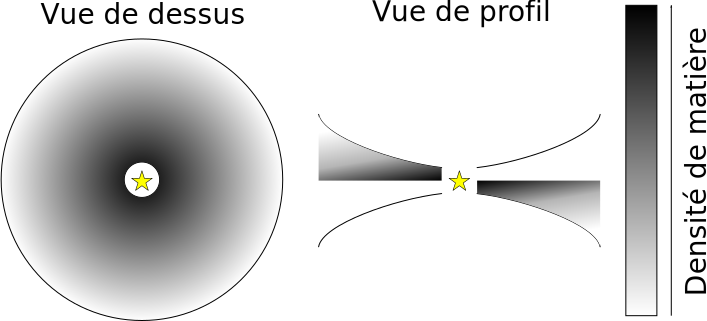
\includegraphics[width=0.45\linewidth]{figure/disk_scheme.pdf}
\caption{Représentation de la répartition radiale et azimutale de matière dans un disque protoplanétaire.}\label{fig:disk_scheme}
\end{figure}

\reffig*{fig:disk_scheme} donne une idée de ce qu'est un disque protoplanétaire. Pour autant, ce n'est qu'une représentation et il est toujours important de garder en tête quelques différences notables entre cette représentation et la réalité physique d'un disque. Quand on parle de disque protoplanétaire, on fait référence à la composante gazeuse, largement majoritaire. Pourtant, bien que minoritaire, la poussière joue un rôle majeur et sa répartition spatiale ne suis pas forcément exactement celle du gaz, ces deux entitées n'ayant pas les mêmes propriétés, elles ne sont pas strictement régies par les mêmes équations.

\bigskip

Tout d'abord, le bord interne est une des parties les plus complexes d'un disque protoplanétaire. Ce bord interne correspond, pour la poussière, à une température de 1500K environ, température au delà de laquelle la partie réfractaire des grains se sublime. 

Le gaz, quant à lui, ne se propage pas non plus jusqu'à la surface de l'étoile en raison du champ magnétique important autour des jeunes étoiles. Le bord interne est ainsi déterminé par le rayon de co-rotation de l'étoile, c'est à dire la distance à laquelle une particule en rotation képlerienne orbite à la vitesse de rotation de l'étoile. Le champ magnétique de l'étoile tournant à la vitesse de rotation de l'étoile, ce rayon de co-rotation correspond ainsi au rayon en dessous duquel le gaz est freiné par le champ magnétique et est rapidement accrété le long des lignes de champ. 

\bigskip

En considérant un système \og étoile + disque\fg isolé, il n'y a pas d'arrêt brutal de la distribution de matière au bord externe qui est donc plus une limitation numérique nécessaire aux simulations qu'autre chose. La réalité est représentée plus fidèlement par une décroissante continue de la matière, difficile à représenter tant pour le bord externe que pour la distribution azimutale du disque. 

Généralement, on considère donc que la taille verticale du disque est égale à une échelle de hauteur (grandeur caractéristique de la décroissance exponentielle verticale de la densité de matière), tandis que la taille radiale du disque dépend de la physique que l'on considère. Dans mon cas j'ai souvent pris un bord externe à 100 AU.


%TODO !!!! Parler de l'équation et parler de manière logique des différents termes et paramètres qui en découlent.

%TODO 
\subsection{Le rôle prépondérant de la poussière}
Le disque est principalement composé de gaz, hydrogène et hélium en majorité. Pour autant, c'est bien la poussière qui est au centre de toutes les attentions, même si cette dernière ne représente qu'1\% de la masse du disque environ.

À cause de la pression quasi inexistante dans le disque en raison des faibles densités, solide et gaz sont les seules phases existantes, il n'y a pas de liquides dans l'espace. La poussière représente la matière solide du disque, en grain plus ou moins fin, allant du nanomètre, micromètre, jusqu'à des tailles planétaires en fin de formation. 

Cette poussière est un composé extrêmement complexe à manipuler. Elle contient différents composés solides en fonction de la température (à certaines températures et densité des composés se volatilisent et d'autres non). La ligne des glaces est une ligne imaginaire au delà de laquelle de la glace d'eau apparait, augmentant de manière drastique la quantité de poussière dans le disque. 

\bigskip

De plus, la poussière est aussi responsable de l'opacité du disque, c'est à dire sa capacité à laisser passer ou non la lumière. À travers l'opacité, la poussière a donc une influence sur la température du disque qui se refroidit plus ou moins efficacement, et qui absorbe le rayonnement stellaire plus ou moins efficacement. 

\subsection{La viscosité du disque} \index{viscosité}% (Franck et al. 1992)
Quand on parle de viscosité $\nu$ dans un disque, ce n'est pas la viscosité moléculaire classique, bien trop faible aux densités rencontrées. On suppose généralement une viscosité due aux turbulences qui est beaucoup plus importante que la viscosité moléculaire, mais qui peut être traitée par les mêmes équations. 

Ceci implique par contre qu'il y ait de l'ionisation. En effet, sans ionisation, il n'y a pas de couplage entre le champ magnétique et la matière, et donc pas de turbulence induite par ce même champ. 

Dans la pratique, il est rare que la viscosité soit calculée de manière cohérente, ce qui serait beaucoup trop couteux en calculs, sans apporter forcément beaucoup plus de précisions étant donné les nombreuses incertitudes sur la poussière, le couplage et le champ magnétique. 

La première hypothèse est de considérer une viscosité constante. Faute de mieux, c'est ce qui semble être le plus évident. On peut, si on veut affiner, utiliser une théorie dite des \gras{disque-alpha}

\subsubsection{Les disques alpha}
On peut introduire un paramètre adimensionné $\alpha$ \citep{shakura1989black}. Dans ce formalisme, plusieurs hypothèses sont faites : 
\begin{itemize}
\item On considère que les turbulences sont sub-soniques.
\item L'échelle des tourbillons des turbulences est plus petite que l'échelle de hauteur du disque
\end{itemize}
Le mécanisme qui a le plus de chance d'être à l'origine de la viscosité alpha est l'\gras{Instabilité Magnéto-Rotationnelle} (MRI). 

\bigskip

En conséquence, on peut définir la viscosité $\nu$ associée aux turbulences comme étant 
\begin{align}
\nu &= \alpha c_s H
\end{align}
où $c_s$ est la vitesse du son et $H$ l'échelle de hauteur du disque. $\alpha$ (avec $\alpha < 1$) est alors un paramètre adimensionné qui permet de définir plus ou moins l'intensité des turbulences, et donc la viscosité qui leur est associée. Une valeur typique d'$\alpha$ se situe entre $10^{-2}$ et $10^{-4}$.

Même si cette prescription simplifie un peu le problème, il semble probable qu'$\alpha$ ne soit pas constant, et dépende de la position dans le disque. On déplace alors le problème, vu que se pose la question des variations d'$\alpha$ dans le disque, notamment la dépendance radiale de ce dernier.

\subsection{Ionisation et dead-zones}\index{ionisation}\index{dead zone}
Pour qu'une instabilité magnéto rotationnelle ait lieu, c'est à dire qu'il y ait un couplage entre le champ magnétique et les mouvements du disque, il faut qu'une partie au moins du disque soit ionisé. Dans ces régions ionisées, on pourra alors avoir transport du moment angulaire via la viscosité due au champ magnétique (et turbulences engendrées). 

Or, comment ioniser? Que ce soit le rayonnement X de l'étoile centrale, des rayons cosmiques ou l'ionisation thermique, il n'est pas si évident que ça de se représenter l'ionisation totale du disque de gaz. Il est donc probable que certaines zones du disques ne soient pas ionisés, et donc que le transport du moment angulaire s'y fasse peu ou pas du tout. Ces zones, appelées \index{dead zone}, sont donc des zones sans viscosité magnétique. %TODO compléter la partie dead zone

\begin{figure}[htb]
\centering
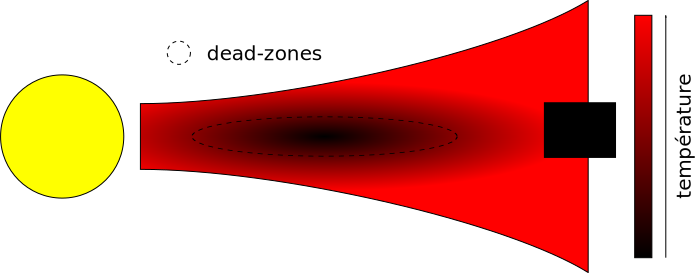
\includegraphics[width=0.7\linewidth]{figure/dead_zones.pdf}
\caption{Représentation d'un disque à couches (layered disk). L'ionisation d'une zone est déterminé par sa température. Ainsi, les zones internes à température plus faible ne sont pas ionisés et n'ont donc pas de viscosité dûes aux turbulences magnétique (MRI). Les régions externes ne sont pas des zones mortes parce qu'elles peuvent être sujettes à des ionisations non thermiques en raison de leur densité plus faible. À distance intermédiaire, le disque est trop froid pour de l'ionisation thermique, et trop dense pour de l'ionisation non thermique.}\label{fig:dead_zones}
\end{figure}


%TODO j'en suis à la page 158 du .pdf ``accretion processes in star formation''

\subsection{Profil de densité}
%TODO 
\subsection{Profil de température}
Du point de vue de la température, il y a principalement deux types de disques : 
\begin{itemize}
\item les \gras[disque actif]{disques actifs} : la source de température est le disque lui même, qui par frottements visqueux (on appelle ça le \gras{chauffage visqueux}) va émettre de la chaleur, et donc chauffer le disque ;
\item les \gras[disque passif]{disques passifs} : la source de chaleur/température est l'étoile centrale qui éclaire le disque. 
\end{itemize}

Un disque peut à la fois être actif et passif, mais généralement on essaie d'approximer, de considérer que l'un est négligeable devant l'autre. De plus, un disque aura des zones actives et des zones passives, c'est à dire que certaines zones seront principalement chauffées par la viscosité alors que d'autres le seront par l'\gras{irradiation de l'étoile}.
%TODO parler de la température du disque (et les phénomènes principaux qui ont un effet sur la température, chauffage visqueux, irradiation de l'étoile, irradiation externe. Parler dans cette partie de l'opacité, des transitions et à quoi c'est dû, des modèles had oc pour l'opacité et des incertitudes qui en découlent

\subsection{Les bords du disque}
%TODO parler des bords du disque et de tous les problèmes que ça pose

\section{Interaction disque-planète}
\subsection{Migration planétaire}
%TODO 
\subsubsection{Type I}\index{migration!type I}
Ce type de migration ne concerne que les planètes de faible masse (de l'ordre de $10M_{\oplus}$)pour lesquelles l'interaction de marée entre la planète et le disque a une réponse linéaire (Le profil de densité surfacique reste quasiment le même). Ces planètes, qui ne creusent pas de sillon (gap) dans le disque de gaz, vont migrer vers l'intérieur.

\begin{remarque}
Pour plus de détails, se référer au chapitre 9, page 188--191 de \cite{barnes2010formation} ou \cite{ward1997protoplanet} pour l'article original.
\end{remarque}

La présence d'une planète dans un disque de gaz entraine la création d'ondes de densités aux \gras[résonnance!de Lindblad]{résonances de Lindblad} \citep{goldreich1979excitation}. Le couplage gravitationnel entre les ondes de densité et la planète qui les crées abouti à un \gras{couple} qui agit sur la planète.

Lors de la création d'ondes de densité par une planète dans un disque, il se forme un déséquilibre naturel entre les couples agissant sur les disques internes et externes. La position des résonances de Lindblad externes tend à être plus proche de la planète que ne l'est celle des résonances internes.


%TODO 
\subsubsection{Type II}\index{migration!type II}
Quand une planète dans un disque devient suffisamment massive, la réponse du disque n'est plus linéaire, et des ondes de densité induites par la planète forment des chocs non loin de là où elles sont émises. La répulsion entre le disque et la planète devient si forte qu'une cavité annulaire se forme autour de l'orbite de la planète, creusant le disque de gaz.

Une fois que la cavité est formée, la planète est dite en migration de \emph{type II} : son orbite agit alors essentiellement comme une barrière entre les deux parties du disque de gaz, \emph{interne} et \emph{externe}. Du gaz peut parfois sauter le gap, ou être accrêté par la planète mais cette dernière voit son mouvement régit par le disque de gaz, se retrouvant entraînée par la migration de celui-ci.

Compte tenu que la planète a une masse de l'ordre de\footnote{Quand la masse de la planète devient supérieure à la masse du disque local, l'inertie de celle-ci devient importante afin de déterminer son taux de migration} la masse du disque local (avec lequel elle interagit), la migration se passe sur des temps de l'ordre du \gras{temps visqueux} du disque.

\begin{remarque}
Pour plus de détails, se référer au chapitre 9, page 191--192 de \cite{barnes2010formation} ou \cite{lin1986tidal} pour des détails sur les planètes capables de former un sillon dans le disque de gaz.
\end{remarque}
%TODO 
\subsubsection{Type III}\index{migration!type III}

%TODO faire ya page 192 du bouquin de barnes un truc sur \c ca, même si c'est pas explicite dans le titre.

\begin{remarque}
Pour plus de détails, se référer au chapitre 9, page 192--193 de \cite{barnes2010formation} ou \cite{masset2003runaway}.
\end{remarque}
%TODO 

\subsection{L'amortissement de l'excentricité}%circularisation
%TODO parler des autres phénomènes importants dans le disque, comme l'amortissement de l'excentricité

\subsection{L'amortissement de l'inclinaison}%coplanarisation
%TODO parler de l'amortissement de l'inclinaison, 

\subsection{L'accrétion du gaz}\label{sec:accretion_coeur}
Dans le modèle d'\gras[modèle!accrétion de c\oe ur]{accrétion de c\oe ur}, les planètes géantes sont d'abord des c\oe urs rocheux qui grossissent jusqu'à atteindre une masse critique de l'ordre de $15 M_{\oplus}$. Une fois cette masse atteinte, le c\oe ur commence à accréter rapidement du gaz jusqu'à former une géante gazeuse.

Ceci implique que la formation des planètes géantes doive se passer avant que le disque de gaz ne se dissipe (ce qui intervient au bout de $10^7$ ans environ).

Les noyaux de ces planètes sont supposés se former au delà de la ligne des glaces (limite radiale virtuelle au delà de laquelle on peut trouver de l'eau sous forme solide ; autour de $4\unit{ua}$). En effet, au delà de cette limite, la quantité de matière solide augmente, et donc le taux d'accrétion augmente aussi.

\begin{attention}
La formation des embryons de planètes géantes n'est toujours pas clair. On ne sait pas vraiment s'il y a une zone privilégiée ou non, la limite virtuelle de la ligne des glaces pourrait ne pas être valable, la glace ne rajoutant qu'environ 50\% de masse en plus.\index{ligne des glaces}\index{snowline|see{ligne des glaces}}

À noter qu'il n'y a pas de pression et donc pas de liquide dans l'espace, juste du gaz ou du solide.
\end{attention}

\bigskip

Pour une simulation donnée, si on augmente le taux d'accrétion de la planète, celle-ci sera plus massive, et aura donc une inertie plus grande. Elle mettra donc plus de temps à migrer\index{migration} par migration Type II car son inertie s'y opposera. D'un autre coté, si la planète n'a pas encore créé de gap, la migration de Type I est plus rapide à mesure que la masse augmente. 

%TODO parler de l'accrétion, et du fait que ça va créer des planètes géantes notamment

\subsection{Récapitulatif des interactions dans le code N-corps}
%TODO parler du fait que je ne prend pas en compte l'accrétion de gaz, les gaps, 

\chapter{Le Code N-Corps}\label{sec:code_n-corps}\label{sec:chap2}
Afin d'étudier la formation planétaire et les interactions avec le disque de gaz, j'ai utilisé un code de simulation N-corps, qui permet de regarder l'évolution d'un nombre arbitraire de corps orbitant autour d'un astre central \citep{chambers1999hybrid}. 

Ce choix est apparu naturellement. Au début de ma thèse j'ai fait quelques simulations hydrodynamiques avec le code Genesis développé par Arnaud Pierens. J'ai rapidement constaté que ce genre de simulations, bien que modélisant de manière poussée le disque, ne permettait pas d'étudier de manière approfondie la dynamique planétaire. Le temps de calcul nécessaire pour une simulation limite en effet grandement le nombre de corps ainsi que la durée d'intégration. J'ai donc souhaité me tourner vers un code N-corps, afin de privilégier la dynamique planétaire, et de modifier ce programme afin d'y inclure les effets d'un disque de gaz sur la dynamique planétaire. 

J'ai ainsi gagné en temps de calcul, et j'ai ouvert un vaste champ d'investigation sur les paramètres du disques, le nombre de corps en interaction, me permettant de faire des systèmes planétaires très divers, parfois avoir plusieurs centaines d'embryons pour plusieurs millions d'années, chose impossible dans les simulations hydrodynamiques du début de ma thèse où 20 corps pendant quelques dizaines de milliers d'années était un maximum. 

Ce choix a bien entendu introduit son lot d'incertitudes et d'approximations qui sont discutés dans la partie \refsec{sec:discussion}. La présente section a pour but de présenter le code N-corps que j'ai utilisé ainsi que les différents effets du disque que j'ai modélisé. J'ai avant tout souhaité présenter les parties qui ont des conséquences sur la physique du disque, que ce soit en terme de choix d'un modèle particulier, ou de limitations numériques qu'il est bien de garder à l'esprit quand on interprète les résultats.

\section{Présentation de mercury}
Le code N-corps choisi est le code \textbf{mercury} \citep{chambers1999hybrid}. Ce code offre la possibilité de choisir un algorithme parmi 5 différents (BS, BS2, RADAU, MVS et HYBRID), ayant des propriétés diverses. Dans le cadre de ma thèse, je n'ai utilisé que l'algorithme HYBRID, qui utilise l'algorithme MVS la plupart du temps, mais change pour l'algorithme BS2 lors de rencontres proches. Il est possible de déterminer à quel moment on considère qu'une rencontre est "proche" dans le fichier de paramètre de programme, j'ai laissé le paramètre par défaut. 

La raison de ce changement est assez simple. MVS est un algorithme symplectique, c'est à dire à pas de temps constant, dans lequel on défini un hamiltonien que l'on résout pour faire évoluer les orbites. La conservation de l'énergie est moins bonne que pour un algorithme à pas de temps adaptatif, mais le point très important est que cette conservation de l'énergie est bien meilleure au cours du temps. C'est à dire que là où les algorithmes tels que BS, BS2 et RADAU verront leur erreur sur l'énergie augmenter au cours du temps, les algorithmes symplectiques vont eux voir leur erreur rester plus ou moins constante au cours du temps. 

Dans le cadre de mes simulations, j'ai accordé une importance limitée aux variations d'énergie, étant donné que les couples que l'on rajoute pour simuler la présence du disque de gaz font que l'énergie n'est pas conservée pour une planète donnée. Cependant, il est important de bien résoudre les orbites et c'est ce point qui est le plus crucial ici. En effet, quelques tests ont permis de contraindre le pas de temps minimal qu'il est nécessaire d'avoir en fonction de la distance orbitale d'une planète. La contrainte de pas de temps dans mes simulations vient donc d'une distance minimale en dessous de laquelle les orbites ne sont pas correctement calculées. Cette limite, afin d'éviter tout problème, est choisie pour être en dessous du bords interne du disque de gaz que je défini.

\section{Algorithmes d'intégration}
Dans mercury, il y a cinq algorithmes différents à notre disposition :
\begin{itemize}
\item MVS \citep{wisdom1991symplectic} : un code symplectique\footnote{Basiquement, un code symplectique est un code qui conserve parfaitement l'énergie de par sa définition en terme d'hamiltoniens.}, c'est-à-dire qui conserve l'énergie au cours du temps et dont le pas de temps est fixe (c'est le seul à avoir un pas de temps fixe)
\item BS \citep{stoer1980introduction} : un algorithme à pas de temps variable, réputé robuste et plutôt long à tourner.
\item BS2 \citep{press1992numerical} : Basé sur BS, il présente l'inconvénient de ne pas fonctionner pour les systèmes non conservatifs. Il est censé être deux fois plus rapide que BS.
\item RADAU \citep{everhart1985efficient} : Ne fonctionne pas bien pour les rencontres proches et les orbites très excentriques. Est censé être deux à trois fois plus rapide que BS.
\item HYBRID \citep{chambers1999hybrid} : Ce code utilise MVS en temps normal, puis lors d'une rencontre proche, utilise BS2 afin de résoudre correctement les orbites.
\end{itemize}

Il y a donc principalement deux catégories : les intégrateurs symplectiques où le paramètre fixe est le pas de temps ($h=\cte$) et les intégrateurs N-corps où le paramètre est la précision en terme de conservation d'énergie d'un pas de temps à l'autre (le pas de temps n'étant pas fixe). Ici, seuls MVS et HYBRID utilisent une partie symplectique alors que BS, BS2 et RADAU sont purement N-corps.

\bigskip

On défini le Hamiltonien $H$ de notre problème N-corps comme étant la somme des énergies cinétiques et potentielles de chaque corps : 
\begin{align}
H &= \sum_{i=1}^N\frac{{p_i}^2}{2m_i} -G\sum_{i=1}^N\sum_{j=i+1}^N\frac{m_im_j}{r_{ij}}
\end{align}
où $m_i$ est la masse du corps $i$, $p_i$ son impulsion et $r_{ij}$ la séparation entre les corps $i$ et $j$.

Un intégrateur symplectique est un intégrateur qui au lieu d'appliquer directement le hamiltonien $H$ sur le système, va séparer ce dernier en deux (ou plusieurs parties) et appliquer ces sous-hamiltoniens successivement. Un intégrateur symplectique résoud donc le problème de manière approchée en négligeant les termes croisés des sous-hamiltoniens.

Afin de minimiser l'erreur dû à cette approximation, il faut choisir judicieusement la séparation du hamiltonien afin d'avoir une partie dominante par rapport à l'autre.

Par définition, un algorithme symplectique conserve l'énergie au cours du temps, même si l'énergie fluctue au cours du temps autour d'une valeur moyenne. 

Les intégrateurs symplectiques ont deux avantages importants sur les intégrateurs classiques : 
\begin{enumerate}
\item Les fluctuations \og instantanées\fg de l'énergie dues à un algorithme symplectiques sont plus grandes que celles d'un algorithme N-corps, mais à la différence de ces derniers, l'erreur ne croit pas au cours du temps \reffig{fig:energy_error}.
\item Ils sont moins couteux en temps de calcul, en particulier quand la majeure partie de la masse est contenue dans un seul corps (bien adapté pour l'étude d'un système planétaire autour d'une étoile donc).
\end{enumerate}

\begin{figure}[htb]
\centering
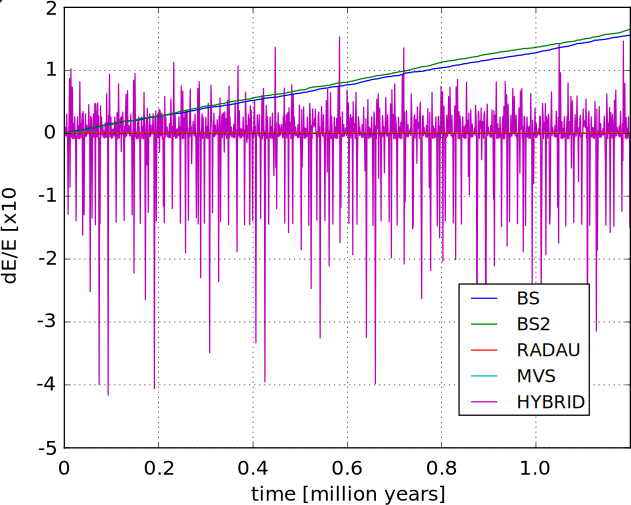
\includegraphics[width=0.65\linewidth]{figure/energy_error.pdf}
\caption{Évolution de l'erreur au cours du temps pour une simulation contenant trois planètes d'une masse terrestre chacune, cette simulation étant lancée successivement avec chacun des algorithmes disponibles dans \textbf{Mercury}.}\label{fig:energy_error}
\end{figure}

Les algorithmes symplectiques ont cependant un inconvénient. Le pas de temps fixe d'un intégrateur symplectique ne permet pas de résoudre correctement les rencontres proches entre les corps du système. Chaque fois que le pas de temps d'un algorithme symplectique est changé, son hamiltonien change aussi, et entraine une variation d'énergie du système (dont l'énergie va osciller autour d'une nouvelle valeur moyenne). 

\bigskip

Nous cherchons maintenant à déterminer l'algorithme le plus approprié pour notre étude. Nous souhaitons faire évoluer un système avec plusieurs dizaines d'embryons planétaire pour plusieurs millions d'années, le système n'étant pas conservatif à cause des divers effets du disque que nous implémentons. 

Nous souhaitons résoudre correctement les orbites, mais avoir un temps de calcul raisonnable. 

La première contrainte est la dissipation. En effet, notre système n'est pas conservatif. Tous les algorithmes N-corps disponibles (BS, BS2 et RADAU) ne fonctionnent donc pas correctement, ces derniers réclament un pas de temps extrêmement faible qui n'est pas représentatif de la précision demandée pour l'intégration N-corps, la variation d'énergie numérique étant masquée par la variation d'énergie induite par les effets du disque. 

Il nous reste les algorithmes MVS et HYBRID. La deuxième contrainte, ce sont les rencontres proches et les collisions. Nous savons qu'un algorithme symplectique ne les traite pas correctement, et si c'est une erreur négligeable dans le cas où il y en a peu, ça ne l'est absolument plus dans notre cas, le nombre de rencontre proche pouvant être très important, notamment dans la phrase d'accrétion en début de simulation. L'algorithme MVS ne parait donc pas adapté contrairement à HYBRID qui a été construit pour être à la fois symplectique et gérer correctement les rencontres proches moyennant une erreur plus importante lors du changement d'algorithme. 

L'algorithme HYBRID est l'algorithme MVS, à pas de temps constant la majorité du temps. Il a donc les avantages d'un algorithme symplectique, à savoir la conservation de l'énergie et la rapidité d'exécution. Lors de rencontres proches (déterminées par une distance minimale d'approche entre deux corps, soit en rayon de Hill, soit en nombre de pas de temps), l'algorithme BS2 est utilisé, le pas de temps devient donc variable afin de résoudre correctement la rencontre et éventuellement la collision. Une fois fini, c'est de nouveau MVS qui prend le relai. 

Dans notre cas, plusieurs approximations sont faites : 
\begin{itemize}
\item L'algorithme BS2 ne fonctionne que pour les systèmes conservatifs. On suppose que la variation d'énergie induite par la migration est totalement négligeable pendant le bref labs de temps de la rencontre proche
\item Le nombre de collisions est suffisamment faible pour que les propriétés symplectiques de l'intégrateur soient conservées. On suppose de plus que les variations d'énergies induites par ce biais sont négligeables devant la dissipation induite par le disque (qui est de l'ordre de l'énergie initiale du système planétaire)
\end{itemize}

Il reste alors une chose à déterminer, c'est le pas de temps fixe que l'on doit choisir afin de résoudre correctement les orbites. Pour cela on se place dans un cas simplifié, sans les effets du disque, et on souhaite savoir la condition sur le pas de temps afin que l'orbite soit correctement calculée. 

%TODO faire des tests numériques, montrer une courbe et donner le nombre minimal de pas de temps nécessaire pour résoudre une orbite correctement et expliquer comme c'est choisi en fonction du bord interne du disque (qui est l'orbite la plus petite atteignable dans notre simulation.




%TODO à partir de là et jusqu'à la fin de la subsection, il faut que je contrôle ce que je dis au regard des simulations lancées et des parties surlignées dans le papier sur hybrid. Notamment à propos de la tolérance aux collisions.

%TODO Simulation lancées dans le dossier $sse/test_mercury, sur une même simulation mais avec différents algorithmes pour voir l'évolution de la conservation de l'énergie au cours du temps

%TODO parler de la précision de conservation de l'énergie
%TODO parler du pas de temps qui a une influence sur les orbites, et des tests effectués pour contraindre le pas de temps par rapport à l'orbite minimale accessible.



\section{Mode d'emploi du code N-corps modifié}
À part la première section qui donne quelques détails techniques, le but de cette partie est de présenter les différentes options du code modifié. Ces options sont lues à partir d'un fichier commun \textbf{disk.in}. Si une option n'est pas présente, la valeur par défaut sera lue à partir du code. Le fichier \textbf{disk.out} récapitule toutes les valeurs de toutes les options et paramètres importants du code. 

\begin{remarque}
Il est possible de mettre des commentaires dans le fichier \textbf{disk.in}, que ce soit pour commenter une ligne entière, ou pour mettre en fin de ligne après un paramètre, à l'aide du caractère \og !\fg exactement comme en Fortran90.
\end{remarque}

\subsection{Note technique}
Le code est en grande partie le code mercury \cite{chambers1999hybrid}. Les effets du disque ont été inclus dans la partie \textbf{mfo\_user} prévue pour inclure des effets propre à chaque utilisateur. 

Pour autant, le code a été conçu de manière modulaire en portant une attention particulière au temps d'exécution et à la souplesse d'utilisation. La plupart des effets sont désactivables par une simple option dans un fichier de paramètre spécifique au effets du disque \textbf{disk.in}. 

Prenons un exemple. Le couple exercé par le disque sur la planète peut être issus des formules de \cite{paardekooper2011torque}, ou bien suivre plusieurs lois artificielles permettant de tester certains effets dans des cas simplifiés. Pour autant, cette souplesse d'utilisation ne se fait pas au détriment de la célérité du code car au lancement du code, les options sont lues et des pointeurs de fonctions permettent au code d'exécuter directement la bonne fonction lors de l'intégration, sans avoir à tester à chaque pas de temps quelle fonction doit être lancée. 

\bigskip

Un programme externe, nommé \textbf{test\_disk} permet d'effectuer des tests unitaires sur différentes fonctions, afin de vérifier quand bon nous semble que chaque fonction n'est pas perturbée par les autres et donne des résultats corrects à la fois physiquement et numériquement.

\subsection{Paramètres divers}
Ici je regroupe des paramètres du disque qui nécessitent simplement une valeur : 
\begin{verbatim}
b/h = 0.6
adiabatic_index = 1.4
mean_molecular_weight = 2.35
disk_edges = 0.1 100.
sample = 800
\end{verbatim}

\textbf{b/h} est la longueur de lissage du potentiel gravitationnel d'une planète (qui diverge dans les simulations hydrodynamiques et qui est un paramètre des formules de \cite{paardekooper2011torque}.

\textbf{adiabatic\_index} est l'indice adiabatique $\gamma$ comme son nom l'indique. De même, \textbf{mean\_molecular\_weight} est la masse moléculaire moyenne $\mu$.

\textbf{disk\_edges} défini les deux extrémités du disque, les bords internes et externes.

\textbf{sample} défini le nombre de points qu'auront les profils radiaux des différents paramètres du disque. Ces points ne sont pas répartis uniforméments, il y a plus de points au bord interne qu'au bord externe, afin d'avoir une évolution plus fine des paramètres en fonction du rayon.

\subsection{Densité de surface}
\textbf{surface\_density} permet de définir le profil en loi de puissance pour la densité de surface : 
\begin{verbatim}
surface_density = 500 0.5
\end{verbatim}
Ici, on a défini le profil suivant : 
\begin{align*}
\Sigma(R) &= 500. \cdot R^{-0.5} \unit{g/cm^2}
\end{align*}

Mais il est aussi possible de donner un profil tabulé de densité de surface en fonction du rayon en paramètre d'entrée, en spécifiant le paramètre suivant : 
\begin{verbatim}
surface_density = manual
\end{verbatim}
Ainsi, le profil de densité de surface sera lu à partir du fichier \textbf{surface\_density\_profile.dat} qui doit être constitué de deux colonnes, la première étant la valeur du rayon en AU, et la deuxième la densité de surface en \unit{g/cm^2}. Les lignes doivent être classées par ordre croissant de distance orbitale. (les premières lignes étant les points les plus proches de l'étoile, et les dernières les points les plus lointains. 

\begin{remarque}
Une interpolation sera réalisée si la discrétisation du fichier d'entrée est différente de celle du code.
\end{remarque}

\bigskip

À ceci s'ajoute un paramètre supplémentaire : 
\begin{verbatim}
inner_smoothing_width = 0.05
\end{verbatim}

Ce paramètre représente la longueur d'amortissement de la densité de surface au bord interne du disque, afin que la densité de surface au bord interne soit très faible. Cette longueur est exprimée en pourcentage de distance orbitale du bord interne ; c'est à dire que si le bord interne est à 0.1 AU, alors dans le cas présent, le lissage sera effectué sur une longueur de 0.005AU

\subsection{Irradiation de l'étoile centrale}
\textbf{is\_irradiation} permet de définir si on veut inclure ou non l'irradiation dans le calcul de l'équilibre énergétique du disque. 

\begin{verbatim}
is_irradiation = 1
disk_albedo = 0.5
r_star = 4.65e-3 ! AU
t_star = 5700 ! K
\end{verbatim}

Les paramètres sont relativement explicite mais pour détailler, \textbf{disk\_albedo} est l'albedo moyen du disque protoplanétaire, il représente le fait qu'une partie de la lumière incidente de l'étoile est directement réfléchie vers l'espace.

\textbf{r\_star} et \textbf{t\_star} sont respectivement le rayon de l'étoile en AU et sa température en Kelvin.

La manière dont est modélisée l'irradiation de l'étoile centrale est détaillée dans \refsec{sec:irradiation}.

\subsection{Viscosité}
Il est possible de définir plusieurs types de viscosité via l'option \textbf{viscosity\_type} : \textbf{constant}, \textbf{alpha} et \textbf{alpha\_dz}.

\subsubsection{constant}
Ce paramètre permet de définir une viscosité $\nu$ constante dans tout le disque. La valeur de la viscosité associée est définie dans le paramètre \textbf{viscosity} en \unit{cm^2/s}.

\begin{verbatim}
viscosity_type = constant
viscosity = 1e15 ! cm^2/s
\end{verbatim}

\subsubsection{alpha}
Ce paramètre permet de définir une viscosité via la prescription alpha de \cite{shakura1973black}. La valeur du paramètre alpha sera lue dans le paramètre \textbf{alpha}. 

\begin{verbatim}
viscosity_type = alpha
alpha = 5e-3
\end{verbatim}

\subsubsection{alpha\_dz}\label{sec:dead_zone}
Ce paramètre permet de définir une viscosité alpha par morceau, permettant de modéliser une dead zone. On aura donc 3 zones avec 3 alpha différents. Pour définir ces zones là, il faut donner dans le paramètre \textbf{alpha\_dz} trois valeurs de $\alpha$ et dans \textbf{radius\_dz} deux valeurs de distance orbitales (en AU) pour définir les bornes de la dead zone.
\begin{verbatim}
viscosity_type = alpha_dz
alpha_dz = 0.005 0.0001 0.005
radius_dz = 1.0 10.0 ! in AU
\end{verbatim}

Quand cette option est activée, une modification au profil de densité est appliquée, afin de modéliser une sous-densité, puis une sur-densité avant et après le bord interne de la zone morte. L'écart maximum de ces \og bumps\fg est de 15\% de la valeur de la densité au bord interne de la zone morte. 

À ceci s'ajoute un lissage des valeurs de $\alpha$ entre la valeur à gauche et la valeur à droite de la transition selon une tangente hyperbolique. La transition s'effectue typiquement sur une longueur égale à 10\% de la position de la transition dans le disque (si la transition est à 1AU, alors la transition a lieu sur 0.1 AU autour de la transition).

\subsection{Opacité}
Afin de pouvoir les comparer, j'ai ajouté au code la possibilité de tourner avec différents modèles pour l'opacité. 

Les différents modèles sont \citep{bell1994FU, zhu2009nonsteady, chambers2009analytic, hure2000transition}

\subsubsection{bell}
\begin{verbatim}
opacity_type = bell
\end{verbatim}

L'opacité est alors calculée en utilisant le modèle fourni par \cite{bell1994FU}. 

\subsubsection{zhu}
\begin{verbatim}
opacity_type = zhu
\end{verbatim}

L'opacité est alors calculée en utilisant le modèle fourni par \cite{zhu2009nonsteady}. 

\subsubsection{chambers}
\begin{verbatim}
opacity_type = chambers
\end{verbatim}

L'opacité est alors calculée en utilisant le modèle fourni par \cite{chambers2009analytic}. Ce modèle est très simplifié et utilisé une opacité constante sur un grand régime de température, pour ensuite faire une transition vers une loi de puissance à très haute température.

\subsubsection{hure}
\begin{verbatim}
opacity_type = hure
\end{verbatim}

L'opacité est alors calculée en utilisant le modèle fourni par \cite{hure2000transition}. 

À la différence de tous les autres modèles que j'ai implémenté, celui de \cite{hure2000transition} est directement une table d'opacité, sans faire intervenir de loi de puissance pour différents régimes. Il n'introduit donc pas d'incertitudes supplémentaire via les loi de puissance qu'il défini. Cette table
d'opacité de Rosseland correspond à la composition suivante $X=0.70$, $Y=0.28$ et $Z=0.02$ et est basée sur
\cite{seaton1994opacities, alexander1994low, henning1996dust}.

En effet, dans le cas qui nous intéresse, c'est à dire la migration planétaire via la formule de \citep{paardekooper2011torque}, l'indice des loi de puissance pour la densité de surface et la température a une très grande influence sur la couple effectif du disque. Et les transitions d'opacités, très marquées lors de la transition des lois de puissance, fait apparaître des zones particulières dans le disque qui n'ont parfois aucune réalité physique mais ont de grandes conséquences sur le résultat des simulations. De même, le lissage qu'elles introduisent masquent certaines zones d'intérêt qui ne sont mises en évidence qu'avec une table d'opacité où tous les effets fins ont été préservés.

\subsection{Turbulence}
Pour activer la turbulence dans le disque, c'est à dire l'effet que la turbulence peut induire sur la migration planétaire, il suffit d'utiliser le paramètre suivant : 
\begin{verbatim}
is_turbulence = 1
\end{verbatim}

La turbulence n'est ici qu'une migration stochastique de moyenne nulle qui perturbe les planètes et leur migration. 

Le modèle utilisé est le même que celui détaillé dans \cite{ogihara2007accretion}. Le principe est de définir un potentiel turbulent dans le disque, fait de la superposition de perturbation individuelle qui ont des modes $m$, temps de vie $t_m$ et position dans le disques différents. 

Dans le cas typique, il y a 100 modes différents dans le disque : 
\begin{align}
\Phi_\text{turb}(R,\phi,t) &= \gamma R^2 \Omega^2 \sum_{k=1}^{100} \Lambda_k(R,\phi,t)
\end{align}
avec 
\begin{align}
\Lambda_k &= \xi_k e^{-\frac{(R-R_k)^2}{{\sigma_k}^2}} \cos\left(m_k \phi -\phi_k - \Omega_k\tilde{t}_k\right) \sin\left(\pi \tilde{t}_k/\Delta t_k\right)
\end{align}

$\xi_k$ est une constante adimensionnée déterminée aléatoirement en suivant une distribution gaussienne.

$R_k$ et $\phi_k$ sont respectivement les coordonnées radiales et azimutales du mode $k$ choisies aléatoirement et de manière uniforme pour l'un entre les bornes du disque, pour l'autre entre $0$ et $2\pi$. 

Chaque mode $k$ possède un nombre de mode $m_k$ déterminée selon une distribution logarithmique entre $m=1$ et $m=150$, le nombre de mode déterminant l'extension radiale et la durée du vie du mode $k$.

$\sigma_k = \pi R_k / 4m_k$ est l'extension radiale de ce mode tandis que $\Omega_k$ représente la vitesse angulaire képlerienne à la position $R=R_k$.

$\Delta t_k=0.2\pi R_k / m_k c_s$ est la durée de vie du mode $k$. 

\bigskip

Les modes apparaissent et disparaissent en fonction de leur temps de vie et sont remplacés afin qu'il y ait toujours 100 modes différents dans le disque à un instant $t$. Chaque mode $k$ est créé à un instant $t_{0,k}$ et se termine quand $\tilde{t}_k = t-t_{0,k} > \Delta t_k$.

\subsection{Migration}
\subsubsection{real}
C'est le cas le plus classique. Il n'y a pas besoin de définir d'autres paramètres, la migration induite par le disque de gaz sera simplement calculée à partir du modèle de \cite{paardekooper2011torque}.

\begin{verbatim}
torque_type = real
\end{verbatim}

\subsubsection{mass\_dependant}
\begin{figure}[htb]
\centering
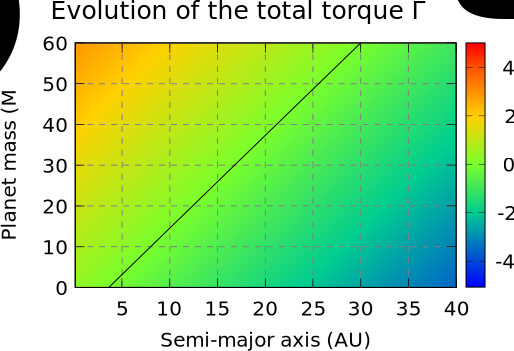
\includegraphics[width=0.65\linewidth]{figure/migration_map/mass_dependant.pdf}
\caption{Cette carte représente l'effet du disque dans le cas de l'option \textbf{mass\_dependant} pour une planète en fonction de sa position en abscisse et de sa masse en ordonnée. La ligne noire représente la zone de couple nul, c'est à dire une zone où la migration de la planète s'arrête.}
\end{figure}

On définit une zone de convergence artificielle qui va dépendre de la masse des planètes. On va donc devoir définir deux bornes en masses et deux bornes en distance orbitale qui vont déterminer cette ligne de couple nul. À l'intérieur (resp. extérieur) de cette séparation virtuelle, la migration sera vers l'extérieur (resp. intérieur).

Ensuite, on défini une pente linéaire plus ou moins importante pour voir à quelle vitesse on va tendre vers la valeur de saturation à mesure qu'on s'éloigne de la zone de convergence. Une pente de $1$ signifie que le couple $\Gamma/\Gamma_0$ augmente de 1 tous les 10 AU.

En résumé, on a ces paramètres suivants à définir : 
\begin{verbatim}
torque_type = mass_dependant

mass_dep_cz_m_max = 30 ! AU
mass_dep_m_max = 60 ! m_earth

mass_dep_cz_m_min = 4 ! AU
mass_dep_m_min = 1 ! m_earth

torque_profile_steepness = 1.0
\end{verbatim}

\subsubsection{linear\_indep}
Même chose que précédemment, on peut définir un couple artificiel qui défini une zone de convergence indépendante de la masse, c'est à dire qu'on ne spécifie que la position de la zone de convergence dans le disque. On a donc : 
\begin{verbatim}
torque_type = linear_indep
indep_cz = 3.0 ! AU
torque_profile_steepness = 1.0
\end{verbatim}

Une pente de $1$ signifie que le couple $\Gamma/\Gamma_0$ augmente de 1 tous les 10 AU.

\begin{figure}[htb]
\centering
\includegraphics[width=0.65\linewidth]{figure/migration_map/linear_indep.pdf}
\caption{Cette carte représente l'effet du disque dans le cas de l'option \textbf{linear\_indep} pour une planète en fonction de sa position en abscisse et de sa masse en ordonnée. La ligne noire représente la zone de couple nul, c'est à dire une zone où la migration de la planète s'arrête.}
\end{figure}

\subsubsection{tanh\_indep}\label{sec:tanh_indep}
Ici, on défini aussi une zone de convergence indépendante de la masse, mais au lieu d'avoir une évolution linéaire du couple à mesure qu'on s'éloigne de la zone de convergence, on a une tangente hyperbolique qui sature à une valeur que l'on peut donner en paramètre. 

La valeur du couple de saturation défini la valeur absolue du couple vers laquelle on va tendre quand on est très loin de la zone de convergence. Si on est à l'extérieur, ce sera cette valeur de saturation prise négativement, tandis que c'est la valeur positive qui est utilisée à l'intérieur.

On a donc les paramètres suivants à définir : 
\begin{verbatim}
torque_type = tanh_indep
indep_cz = 3.0 ! AU
saturation_torque = 1.0 ! in Gamma_0
\end{verbatim}

\begin{figure}[htb]
\centering
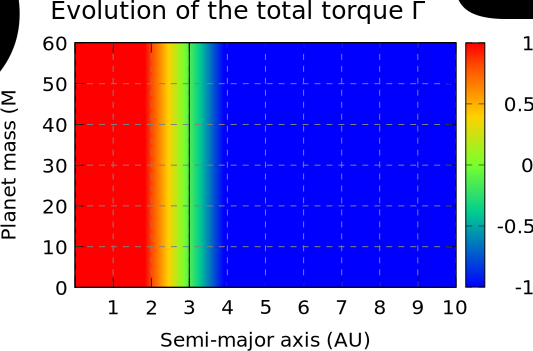
\includegraphics[width=0.65\linewidth]{figure/migration_map/tanh_indep.pdf}
\caption{Cette carte représente l'effet du disque dans le cas de l'option \textbf{tanh\_indep} pour une planète en fonction de sa position en abscisse et de sa masse en ordonnée. La ligne noire représente la zone de couple nul, c'est à dire une zone où la migration de la planète s'arrête.}
\end{figure}

\subsubsection{manual}
Il est aussi possible de rentrer manuellement un couple total en fonction de la position de la planète dans le disque. 

Les valeurs seront alors lues à partir du fichier \textbf{torque\_profile.dat}. La première colonne sera les positions dans le disque en AU tandis que la deuxième colonne sera le couple exercé par le disque en unité de $\Gamma_0$ (c'est à dire que l'effet de la masse de la planète sur la vitesse de migration sera toujours pris en compte dans le code au travers de la dépendance de $\Gamma_0$ en fonction de la masse de la planète et de la masse du disque.

%TODO j'en suis là

\section{Disque 1D}
Afin de calculer les effets d'un disque de gaz, une modélisation de ce dernier est nécessaire. Le but étant d'avoir une grande souplesse, le disque implémenté est bien entendu très simplifié. Toutes les quantités sont intégrées et invariantes selon la hauteur z et la position azimutale $\theta$ dans le disque, résultant en un modèle radial 1D de toutes les quantités. 

Dans la mesure du possible, les quantités du disque ont été calculées de manière consistante. Je vais présenter dans la suite de manière chronologique comment sont calculées les grandeurs physiques du disque.

\subsection{Profil de densité de surface}
Le profil de densité de surface est défini au début de la simulation comme une loi de puissance de la forme :
\begin{align}
\Sigma(R) &= \Sigma_0 \times R^{-d}
\end{align}
où $\Sigma_0$ est la densité de surface à $1\unit{AU}$ et $d$ l'indice de la loi de puissance. 

Ce profil de densité de surface est défini pour une certaine étendue radiale. On défini donc un bord interne $R_\text{in}$ et un bord externe $R_\text{out}$. Le bord interne est généralement à $0.1\unit{AU}$ et le bord externe à $100\unit{AU}$. 

Afin de calculer les valeurs suivantes, ce disque est échantillonné et toutes les valeurs nécessaires sont ensuite calculées à chacun de ces points. 

\bigskip

Le profil de densité de surface est le paramètre d'entrée le plus important. Il est celui à partir duquel on calcule toutes les autres quantités du disque, température, échelle de hauteur, etc\dots

Le profil étant une loi de puissance, un amortissement est effectué au bord interne du disque afin que la valeur de la densité au bord interne soit proche de zéro. 


\subsection{Table d'opacité}
Afin de pouvoir calculer le profil de température, on a besoin de choisir un modèle pour l'opacité. Je ne détaillerai pas ici les différents modèles car une étude complète sur le sujet a été effectuée, afin de comprendre l'influence du choix du modèle sur les résultats des simulations. 

Par contre, quel que soit le modèle, on a généralement une dépendance en fonction de la densité et de la température. L'opacité est donc un paramètre de la résolution de l'équation qui nous permet d'avoir la température. L'opacité n'est pas, dans notre modèle, une quantité qu'on fixe \textit{a priori}, mais plutôt un des paramètres de sortie de la résolution de l'équation de l'énergie dans le disque.

%TODO 
\subsection{Profil de température}
Afin de construire le profil de température point par point, on résout, pour chaque position dans le disque définie dans le profile, l'équation de l'énergie \refeq{eq:equation_energie}. 

De manière consistante, cette équation a pour paramètre d'entrée la position, et on cherche à trouver les valeurs de la température $T$, échelle de hauteur $H$, profondeur optique $\tau$, diffusivité thermique $\chi$. Toutes ces valeurs sont fixées une fois qu'un ensemble cohérent de valeurs satisfont l'équation.

Afin de résoudre cette équation du type $f(x)=0$, j'ai utilisé une version modifiée de la méthode \textbf{zbrent} de \textbf{Numerical Recipes} \citep{press1992numerical}

%TODO 
\section{Migration type I}
La migration de type I est implémentée dans le code en utilisant le modèle 1D de disque, qui définit pour toute position du disque, une température, une densité de surface, et tous les autres paramètres nécessaires comme l'échelle de hauteur. En utilisant ces paramètres, on obtient ainsi le couple qu'exerce le disque sur la planète en fonction de sa masse et de sa position via la formule semi-analytique de \cite{paardekooper2011torque}. 

Les deux différences principales entre le cadre du modèle de \cite{paardekooper2011torque} et le disque que j'ai modélisé, c'est que dans mon cas je n'ai pas un profil de température en loi de puissance (avec une seule loi de puissance), mais j'ai une loi de puissance définie point par point. C'est à dire que pour chaque zone du disque, la température est calculée de manière cohérente avec les autres paramètres du disques, et que l'indice de la loi de puissance correspondante est calculée en fonction des températures autour.

La deuxième différence est que j'ai un profil pour l'échelle de hauteur $H$ et le rapport d'aspect $h=H/R$ du disque au lieu d'avoir un rapport d'aspect constant pour tout le disque.

\bigskip

De plus, certaines erreurs se sont glissées dans ce papier. \cite[appendice A]{bitsch2011range} fait remarquer en particulier qu'il manque un facteur 4 dans l'équation (33). Ainsi, la formule que j'ai utilisé pour calculer la conductivité thermique $\chi$ est :
\begin{align}
\chi &= \frac{16\gamma (\gamma-1) \sigma T^4}{3\kappa \rho^2 H^2\Omega^2}
\end{align}

Il y a aussi une erreur dans l'équation (35) car le disque se refroidit par la surface supérieur et la surface inférieure. Mais comme j'utilise dans mon code une équation de l'énergie \refeq{eq:equation_energie} un peu plus complexe où j'ai tenu compte de ce fait là, cette erreur n'a pas d'incidence sur le calcul du couple.

Les formules nous donnent alors un couple exercé par le disque sur la planète. 

À partir de ce couple, on définit un temps de migration $t_\text{mig}$ comme : 
\begin{align}
t_\text{mig} &= \frac{J}{2\Gamma}
\end{align}
où $J$ est le moment angulaire total de la planète et $\Gamma=\dot{J}$ est le couple total exercé par le disque sur la planète.

L'accélération due à la migration $\vect{a_\text{mig}}$ est alors donnée par :
\begin{align}
\vect{a_\text{mig}} &= \frac{\vect{v}}{t_\text{mig}}
\end{align}
où $\vect{v}$ est la vitesse instantanée de la planète.

\section{Amortissement de e et I}
L'amortissement de l'eccentricité $e$ et de l'inclinaison $I$ d'une planète plongée dans un disque protoplanétaire est modélisée dans le code via les formules de \cite[eq. (9), (11) et (12)]{cresswell2008three} : 
\begin{subequations}
\begin{align}
t_\text{wave} &= \frac{M_\star}{m_p}\frac{M_\star}{\Sigma_p {a_p}^2}\left(\frac{H}{r}\right)^4{\Omega_p}^{-1}\\
t_e &= \frac{t_\text{wave}}{0.780}\left[1-0.14\left(\frac{e}{H/r}\right)^2 + 0.06 \left(\frac{e}{H/r}\right)^3 + 0.18\left(\frac{e}{H/r}\right)\left(\frac{i}{H/r}\right)^2\right]\\
t_i &= \frac{t_\text{wave}}{0.544}\left[1-0.30\left(\frac{i}{H/r}\right)^2 + 0.24 \left(\frac{i}{H/r}\right)^3 + 0.14\left(\frac{e}{H/r}\right)^2\left(\frac{i}{H/r}\right)\right]
\end{align}
\end{subequations}

L'amortissement de $I$ est arrêté quand l'inclinaison descend en dessous de $I<5\cdot 10^{-4}\unit{rad}$ afin d'empêcher les planètes d'être parfaitement dans le plan $(x,y)$, essentiellement pour empêcher des problèmes numériques.

%TODO 
\section{Effet de l'excentricité sur le couple de corotation}
Afin de tenir compte d'un effet mis en évidence par \cite{bitsch2010orbital}, une petite modification a été effectuée dans le calcul du couple total $\Gamma$ exercé par le disque sur la planète. 

En effet, il a été montré que l'excentricité d'une planète a une influence sur sa zone fer-à-cheval et par extension, sur son couple de corotation $\Gamma_C$. Un paramètre d'amortissement $D$, compris entre 0 et 1 a ainsi été ajouté au calcul du couple total :
\begin{align}
\Gamma &= \Gamma_0 \cdot (\Gamma_L + D\cdot \Gamma_C)
\end{align}
où $\Gamma_0 = \left(\frac{q}{h}\right)^2\Sigma_p {r_p}^4 {\Omega_p}^2$ et $\Gamma_L$ est le couple de Lindblad.

La valeur du paramètre d'amortissement $D$ est donnée par une formule qui a été calculée pour coller au mieux aux simulations de \cite{bitsch2010orbital}, détaillée dans \cite{cossou2013convergence}, et recopiée ici : 
\begin{subequations}
\begin{align}
D = \frac{\Gamma_C(e)}{\Gamma_C (e=0)} &= 1 + a \cdot \left[\tanh(c) - \tanh\left(\frac{b * e}{x_s}+c\right)\right]\label{eq:eccentricity-influence}\\
a &= 0.45 \qquad b=3.46 \qquad c= -2.34
\end{align}
\end{subequations}
où $x_s$ représente la demi-largeur de la zone fer-à-cheval divisée par le demi-grand axe.

\section{Désactivation des effets du disque}
Quand une planète sort des bornes du disques, les effets d'amortissement de $e$ et $I$ sont désactivés, au même titre que la migration dû à la présence du disque. Ce cas survient rarement au bord externe du disque (généralement à $100\unit{AU}$), mais est beaucoup plus probable au bord interne (généralement à $0.1\unit{AU}$).

\section{Validité des éléments orbitaux}
Lorsque d'une rencontre proche entre deux planètes, leurs interactions gravitationnelles rendent caduque les formules qui permettent de calculer les éléments orbitaux à partir des vitesses et positions car ceci suppose qu'on est dans le cas d'une orbite képlerienne isolée. 

Dans de tels cas, on peut avoir des demi-grands axe négatifs, des excentricités supérieures à 1. Si c'est déjà en soit un problème physique, c'est aussi et surtout un problème numérique car cela fait apparaître des \textbf{Not A Number} (NaN) quand par exemple on a le demi-grand axe en argument d'une racine carrée. Ceci a donc pour conséquence concrète de faire planter le code, au mieux, ou pire, de le faire tourner avec tous les paramètres de la simulation peu à peu gangrénés par des \textbf{NaN}. 

En conséquence, j'ai décidé de remplacer dans la plupart des calculs de mes simulations, le demi-grand axe par le rayon $r=\sqrt{x^2+y^2+z^2}$ qui lui n'est pas sensible à ce genre de divergences. Quand il y a une excentricité, il est clair que le rayon est différent du demi-grand axe. Mais les excentricités étant généralement faible, l'erreur faite sur le demi-grand axe reste faible. De plus les rencontres proches représentent un temps négligeable de la simulation au regard des centaines de milliers d'années sur lesquelles on intègre les orbites. On considère donc que la migration induite sur les planètes pendant leur temps de rencontre proche est totalement négligeable au regard du reste de la simulation.


%TODO j'en suis là.

%TODO du couple de corotation quand l'excentricité augmente, mais je sais pas encore où le placer, pas dans la partie intro je suppose


\chapter{Cartes de migration}\label{sec:chap3}\index{carte de migration}
Dans les disques radiatifs, la migration de type I est gouvernée par le couple différentiel de Lindblad, qui induit généralement
une migration vers l'intérieur \citep{tanaka2002three}, et le couple de corotation qui peut contrebalancer le couple
différentiel de Lindblad sous certaines conditions et ainsi inverser le sens de migration (vers l'extérieur)
\citep{paardekooper2006halting, kley2008migration}. Il est donc possible d'avoir dans un disque des zones où la migration
s'arrête. Ces zones sont appelées zone de convergence \citep[CZs;][]{lyra2010orbital, mordasini2011application,
paardekooper2011torque}. 

\bigskip

À la zone de convergence, le couple de corotation (positif) compense exactement le couple différentiel de Lindblad (négatif).
Ainsi, à la zone de convergence, une planète ne migre pas.

De plus, autour de la zone de convergence, la migration tend à ramener les embryons vers la zone de couple nul s'ils s'en
éloignent. La zone de convergence est donc une position stable dans le disque vers laquelle les embryons se rassemblent.

Il peut exister de même des zones de couples nuls qui ne sont pas des zones de convergence quand, en s'éloignant légèrement, la
migration tend à les éloigner davantage. Ces zones sont alors instables.

Les zones de convergences pourraient ainsi concentrer les embryons planétaires et être le lieu de formation de planètes (ou
cœurs) massives \citep{lyra2010orbital, horn2012orbital}. 

\section{Disque de référence}\label{sec:migrations-maps}\label{sec:reference_disk}
%TODO parler des raisons pour lesquelles la zone de convergence dépend de la masse et de la distance parfois, avec les
%comparaisons des temps (dynamique, de U-turn and de diffusion)

\begin{figure}[htb]
\centering
\includegraphics[width=0.75\linewidth]{figure/migration_map/fiducial.pdf}

\caption{Carte de migration pour le disque fiducial. Cette carte montre le sens de migration d'une planète en fonction de sa
position (abscisse) et de sa masse (ordonnée). La 3\ieme coordonnée est le couple total exercé par le disque sur la planète,
exprimé en unité de $\Gamma_0 = \left(\frac{q}{h}\right)^2\Sigma_p {r_p}^4 {\Omega_p}^2$. Quand le couple est positif (resp.
négatif), la migration est vers l'extérieur (resp. intérieur). La ligne noire représente la zone de couple nul, où la planète ne
migre plus. Le détail des paramètres du disque de référence est donné \reftab{tab:fiducial_parameters}.
}\label{fig:fiducial_migration_map}
\end{figure}

Dans cette section, nous allons présenter notre disque de référence et comment ses paramètres vont influencer la migration des
planètes. Ce disque de référence servira aussi de comparaison quand nous étudierons les effets des paramètres du disque.

Afin d'étudier la migration dans les disques, il est pratique de regarder une \og carte de migration\fg, comme
\reffig{fig:fiducial_migration_map}. Cette carte permet de voir rapidement les parties intéressantes et de prédire l'évolution
d'une planète à partir de la position et masse initiales.

\reffig{fig:fiducial_migration_map} montre la carte de migration du disque de référence que nous utiliserons de manière
récurrente ici. Ce disque est obtenu à l'aide de la table d'opacité d'\cite{hure2000transition}. Le profil de température est
calculé en tenant compte de l'irradiation, avec des paramètres solaires pour la température et le rayon de l'étoile ($T_\star =
5700\unit{K}$ ; $R_\star = 4.65\cdot 10^{-3}\unit{AU}$). L'albédo du disque est pris égal à $0.5$. La viscosité est calculée à
partir d'une prescription alpha \citep{shakura1973black}. On considère un disque dont les bords internes et externes sont
respectivement à $0.1$ et $100\unit{UA}$. Les autres paramètres du disques sont récapitulés \reftab{tab:fiducial_parameters}. 

\begin{table}[htb]
\centering
\begin{tabular}{|c|c|c|c|}
\hline
$b/h = 0.4$ & $\gamma = 7/5$ & $\mu = 2.35$ & $\alpha = 5\cdot 10^{-3}$ \\\hline
\multicolumn{2}{|c|}{Inner edge : $0.1\unit{UA}$} & \multicolumn{2}{c|}{Outer edge : $100\unit{UA}$}\\\hline
\multicolumn{4}{|c|}{$\Sigma(R) = 300 \cdot R^{-1/2}\unit{g/cm^2}$}\\\hline
$T_\star = 5700\unit{K}$ & $R_\star = 4.65\cdot 10^{-3}\unit{AU}$ & \multicolumn{2}{c|}{Disk albedo : $0.5$}\\\hline
\end{tabular}
\caption{Paramètres physiques du disque fiducial. Les opacités sont calculées à partir de la table d'opacité de
\cite{hure2000transition}. La viscosité est calculée en suivant la prescription alpha de
\cite{shakura1973black}.}\label{tab:fiducial_parameters}
\end{table}

\begin{figure}[htb]
\centering
\subfloat[Lindblad torque]{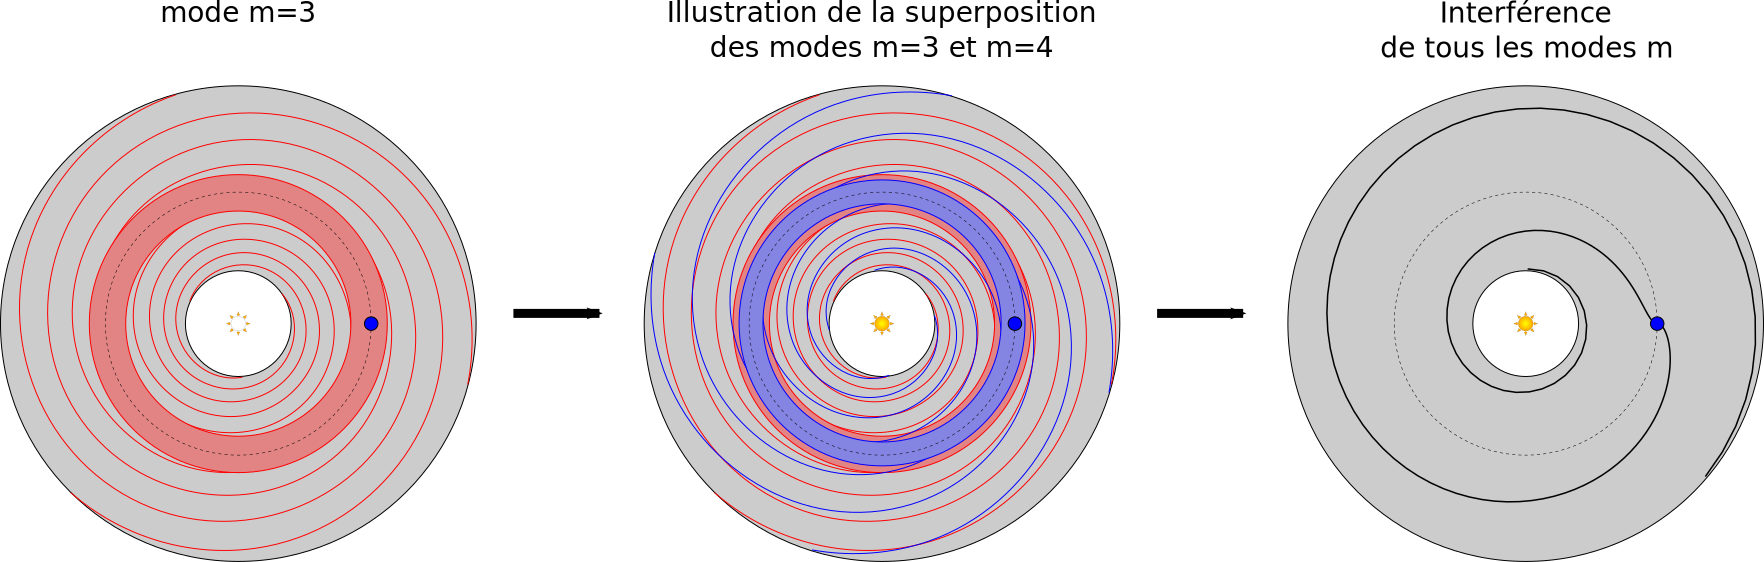
\includegraphics[width=0.49\textwidth]{figure/migration_map/details/lindblad_torque.pdf}}\hfill
\subfloat[Horseshoe Entropy related torque]{\includegraphics[width=0.49\textwidth]{%
figure/migration_map/details/ent_hs_torque.pdf}}

\caption{Evolution des deux couples les plus importants vis à vis de la carte de migration, le couple de Lindblad et la partie
non saturée du couple de corotation liée au gradient d'entropie. En effet, ces deux couples sont quantitativement plus grand que
tous les autres. Ici, seule la partie non-saturée du couple de corotation est représentée.}\label{fig:details_maps}
\end{figure}

Sur \reffig{fig:details_maps} sont représentés les deux couples les plus importants en terme d'amplitude. D'une part le couple négatif dominant, le
couple de Lindblad $\Gamma_L$. Et d'autre part le couple positif dominant, la partie du couple de corotation non saturée liée au gradient d'entropie
$\Gamma_\text{ent,hs}$. Ici, c'est bien la partie non saturée qui est représentée \og fully unsaturated\fg. On ne tient pas
compte de la diffusion. On constate alors que sans tenir compte de la diffusion, les couples sont totalement indépendants de la
masse. La transition que l'on constate dans les deux cartes, entre $6-8\unit{UA}$ correspond à la transition disque
actif/passif. L'irradiation est le processus de chauffage principal à partir de $5\unit{UA}$ comme illustré par
\reffig{fig:viscous_vs_irradiation}.

\begin{figure}[htb]
\centering
\subfloat[$t_\text{rad}/t_\text{U-turn}$]{\label{fig:linear_rad}\includegraphics[width=0.49\textwidth]{%
figure/timescales/linear_rad.pdf}}\hfill
\subfloat[Saturation : $(t_\text{lib}/2)/t_\text{visc}$]{\label{fig:sat_visc}\includegraphics[width=0.49\textwidth]{%
figure/timescales/sat_visc.pdf}}

\caption{Comparaison des différents temps caractéristiques influençant le couple de corotation. Ces inéquations sont détaillées
dans \refsec{sec:couple-corotation}. Dans le cas présent, le temps de diffusion radiative est toujours plus court que le temps
de diffusion visqueuse, $t_\text{rad}<t_\text{visc}$. Ainsi il ne reste plus que les deux inégalités représentées
ici. La saturation est ainsi gouvernée par le temps de diffusion visqueux $t_\text{visc}$. La transition couple non-saturé/couple linéaire est elle déterminée par le temps de diffusion radiatif $t_\text{rad}$.}\label{fig:timescales_maps}
\end{figure}

\reffig{fig:timescales_maps} représente l'effet de la diffusion sur la carte de migration. Comme $t_\text{rad}<t_\text{visc}$, la saturation est gouvernée par le temps de diffusion visqueux $t_\text{visc}$ et la transition couple non-saturé/couple linéaire est déterminée par le temps de diffusion radiatif $t_\text{rad}$. Ainsi, seules deux inégalités sont ici nécessaires pour étudier le couple de corotation :
\begin{align}
t_\text{U-turn} < t_\text{diff} < \frac{t_\text{lib}}{2}\\\nonumber
t_\text{U-turn} < t_\text{rad} < t_\text{visc} < \frac{t_\text{lib}}{2}
\end{align}

Sur \reffig{fig:timescales_maps} on remarque que les parties active et passive du disque sont distinctes. En dessous de $4\unit{UA}$, la partie supérieure de la carte de migration s'explique par la saturation du couple de corotation. La ligne de couple nul suit en effet l'équation $(t_\text{lib}/2) = t_\text{visc}$ \reffig{fig:sat_visc}.

La partie inférieure quant à elle, s'explique par la transition entre le couple non saturé et le couple linéaire pour le couple de corotation. La ligne de couple nul suit en effet l'équation $t_\text{U-turn} = t_\text{rad}$ \reffig{fig:linear_rad}. Le couple de corotation devient linéaire quand le temps de diffusion radiatif est trop court pour permettre à un gradient de s'installer dans la zone de \og U-turn\fg.

\begin{figure}[htb]
\centering
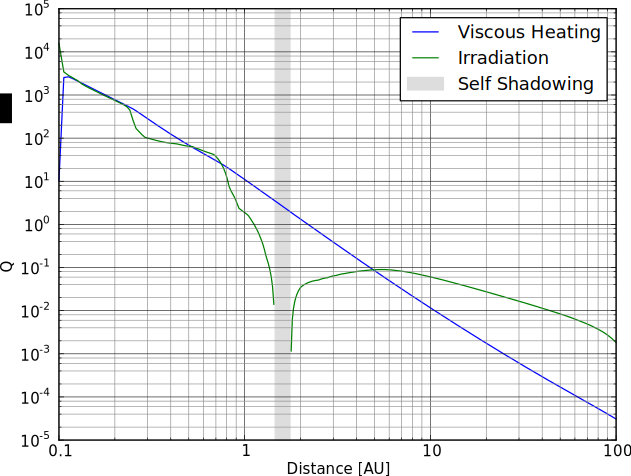
\includegraphics[width=0.75\textwidth]{figure/migration_map/viscous_vs_irradiation.pdf}

\caption{Évolution du chauffage visqueux et de l'irradiation en fonction de la distance. Dans les parties internes, c'est le
chauffage visqueux qui domine. Dans les parties externes c'est l'irradiation. À $5\unit{UA}$ les deux contributions sont
égales. La partie grisée correspond à la zone où l'irradiation est forcée à 0 car l'angle d'interception des rayons solaires est négatif (l'échelle de hauteur diminue). Ce n'est donc pas à proprement parler un \og Self-Shadowing\fg qui concerne une zone beaucoup plus étendue.}\label{fig:viscous_vs_irradiation}
\end{figure}

\reffig{fig:viscous_vs_irradiation} montre qu'au delà de $5\unit{UA}$ l'irradiation domine le bilan énergétique du disque. Cela
correspond à la distance à laquelle les cartes mettant en jeu les temps de diffusions n'expliquent plus la forme de la carte de
migration. À partir de cette distance là, l'irradiation modifie la carte de migration. 

À partir de $4\unit{UA}$, ce n'est plus seulement les temps de diffusions qui permettent de trouver la zone de couple nul dans le disque, mais les valeurs des couples eux mêmes. La saturation influe sur le couple de corotation, afin d'en atténuer la valeur en fonction des rapports des temps caractéristiques. Mais au delà de $4\unit{UA}$, les couples augmentent (sans tenir compte de la saturation). 

La fermeture des parties externes de la carte de migration s'explique par l'action conjointe des deux temps de diffusions. Pour les masses
faibles, en dessous de $15-20\mearth$, la migration vers l'intérieur est dur au fait que $t_\text{U-turn} > t_\text{rad}$, c'est
alors la valeur linéaire du couple de corotation qui prévaut. Pour les masses plus importantes, le couple de corotation sature
car $(t_\text{lib}/2) < t_\text{visc}$. 

Les couples dominants variant très fortement avec la distance au delà de $4\unit{UA}$ \reffig{fig:details_maps}, la ligne de couple nul n'est plus confondue avec celle de l'égalité des temps caractéristiques \reffig{fig:timescales_maps}.

Avant $1\unit{UA}$, deux régions de couples positifs sont séparés par une région peu étendue où la migration est vers l'intérieur. C'est une transition d'opacité à $1\unit{UA}$ environ qui
en est la cause, et qui change brusquement les couples de migration, quelle que soit leur origine \reffig{fig:details_maps}. Ce
brusque changement d'opacité et de température est la raison de la séparation de la zone de couple positif en deux. Ainsi, les
raisons qui expliquent la fermeture de la carte de migration à $15\unit{UA}$ sont les mêmes ici. Mais la variation du couple en fonction de la distance est beaucoup plus
grande, de sorte que la position de la zone de convergence semble ne pas dépendre de la masse, contrairement aux parties
externes de la carte de migration.

\section{Différents types de zone de convergence}\label{sec:CZ-types}
En fonction de la distance, nous pouvons définir des masses critiques extrémales au delà desquelles la migration vers
l'extérieur est impossible en raison du temps de diffusion qui est soit trop grand (saturation) soit trop petit (couple
linéaire) pour qu'un couple de corotation non saturé puisse exister.

Mais l'information la plus importante de ces cartes de migration est l'évolution des différentes zones de couple nul en fonction de la
distance. Ces zones sont représentées par une ligne noire. Nous pouvons dégager deux types particulier de zones de convergence. 

Le premier type de zone de convergence est ce que nous appellerons une \textbf{zone de convergence indépendante de la masse}. C'est une
zone qui se trouve plutôt dans les parties interne du disque. Cette ligne de couple nul dépend très peu de la masse de la
planète car une transition d'opacité induit de brusques changements de température. Les couples varient ainsi fortement sur une
distance très courte. Cette zone de convergence a deux caractéristiques importantes : 
\begin{enumerate}
\item La position de la zone de convergence ne dépend pas ou peu de la masse de planète
\item La variation du couple de migration autour de la zone de convergence est très forte
\end{enumerate}

Nous pouvons appeler le deuxième type \textbf{zone de convergence dépendant de la masse}. En effet, dans les parties externes, le
couple varie plus doucement en fonction de la distance. L'influence de la masse est donc plus marqué dans la position de la zone
de couple nul. Ce type de zone de convergence a deux caractéristiques importantes : 
\begin{enumerate}
\item La position de la zone de convergence dépend de la masse de la planète. 
\item Le couple de migration varie doucement en fonction de la distance à la zone de convergence
\end{enumerate}

\begin{figure}[htb]
\centering
\includegraphics[width=0.75\linewidth]{figure/total_torque_fixed_m.pdf}
\caption{Évolution du couple total exercé par le disque sur une planète de $7.5\mearth$. }\label{fig:total_torque_fixed_m}
\end{figure}

\reffig{fig:total_torque_fixed_m} illustre les deux zones de convergences. La première près de $1\unit{UA}$, siège d'une
variation brutale du couple de migration, et la deuxième (dont la position dépend de la masse de la planète) où la variation du
couple de migration est continue. 

Dans la suite, nous avons parfois utilisé des zones de convergences artificielles afin de simplifier les effets, et d'étudier
plus facilement un phénomène particulier. Dans le cas d'une transition d'opacité, nous avons modélisé les zones de convergence
indépendantes de la masse par une tangente hyperbolique dont le zéro se situe à la zone de convergence, et où le couple de
migration (positif ou négatif) sature très loin de la zone de convergence \refsec{sec:tanh_indep}. Pour modéliser une zone de
convergence indépendante de la masse où le couple varie peu autour de la zone de convergence, nous avons utilisé une variation
linéaire du couple de migration \refsec{sec:linear_indep}.

Les zones de convergence dépendantes de la masse peuvent être approximées par une variation linéaire de la position de la zone
de couple nul en fonction de la masse. Le couple de migration varie quant à lui linéairement en fonction de la distance
\refsec{sec:mass_dependant}. 

\section{Influence de la viscosité du disque}
\subsection{Viscosité constante}

\begin{figure}[htb]
\centering
\subfloat[$\nu=10^{14}\unit{cm^2/s}$]{\label{fig:nu_1e14}\includegraphics[width=0.49\textwidth]{figure/migration_map/viscosity/constant_1e14.pdf}}
\hfill
\subfloat[$\nu=5\cdot 10^{14}\unit{cm^2/s}$]{\includegraphics[width=0.49\textwidth]{figure/migration_map/viscosity/constant_5e14.pdf}}


\subfloat[$\nu=10^{15}\unit{cm^2/s}$]{\label{fig:nu_1e15}\includegraphics[width=0.49\textwidth]{%
figure/migration_map/viscosity/constant_1e15.pdf}}\hfill
\subfloat[$\nu=5\cdot 10^{15}\unit{cm^2/s}$]{\label{fig:nu_5e15}\includegraphics[width=0.49\textwidth]{figure/migration_map/viscosity/constant_5e15.pdf}}
\caption{Influence de la viscosité sur la carte de migration. \refdisk}
\end{figure}\label{fig:constant_viscosity}

Le couple de migration est sensible à la valeur de la viscosité $\nu$ \reffig{fig:constant_viscosity}. La viscosité, en modifiant le temps de diffusion visqueux, agit sur la saturation du couple de corotation. Quand la viscosité augmente, le temps de diffusion visqueux $t_\text{visc}$ diminue. Le couple de corotation ne sature pas tant que $(T_\text{visc} < t_\text{lib}/2)$. Si on augmente la viscosité $\nu$, le couple de corotation sature moins facilement à mesure que la masse de la planète augmente. La partie supérieure de la carte de migration se décale vers le haut quand la viscosité augmente. 

Mais l'augmentation de la viscosité a un effet indirect sur le temps de diffusion radiatif $t_\text{rad}$. Si la viscosité augmente, le chauffage visqueux augmente. La température augmente, et la diffusivité thermique $\chi$ avec. Ainsi, quand la viscosité augmente, le temps de diffusion radiatif $t_\text{rad}$ diminue. Le couple de corotation est linéaire quand $t_\text{rad} < t_\text{U-turn}$. Quand la viscosité $\nu$ augmente, le couple de corotation se linéarise plus rapidement à mesure que la masse de la planète diminue. La partie inférieur de la carte de migration se décale elle aussi vers le haut. Des planètes de faibles masses qui migraient vers l'extérieur ne peuvent plus migrer que vers l'intérieur à mesure que la viscosité augmente. 

\subsection{Viscosité alpha}
La prescription alpha \citep{shakura1973black} est une autre manière de définir la viscosité, à partir d'un paramètre adimensionné $\alpha$ \refsec{sec:viscosite-alpha}.

\begin{figure}[htb]
\centering
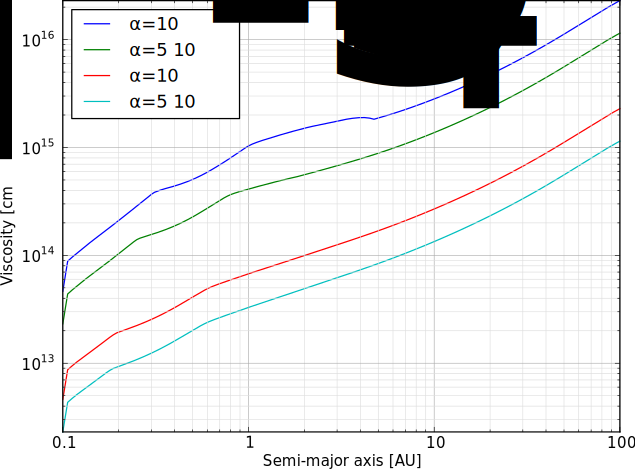
\includegraphics[width=0.6\linewidth]{figure/migration_map/viscosity/alpha_profiles.pdf}
\caption{Profils de viscosité du disque en fonction de la valeur de alpha. Ces profils correspondent à chacune des quatre cartes de migration
présentées \protect\reffig{fig:alpha_viscosity}. \refdisk}\label{fig:alpha_profiles}
\end{figure}

Par rapport à un modèle où la viscosité est constante, la prescription alpha entraine une augmentation continue de la viscosité en fonction de la distance \reffig{fig:alpha_profiles}. Pourtant ce n'est pas un simple facteur multiplicateur de la viscosité en raison du fait qu'il y a maintenant une dépendance en température au travers de l'échelle de hauteur et la vitesse du son. Les variations de $\alpha$ peuvent ainsi faire apparaître des transitions d'opacités au sein même du profil de viscosité. 

\begin{figure}[htb]
\centering
\subfloat[$\alpha=10^{-2}$]{\includegraphics[width=0.49\textwidth]{figure/migration_map/viscosity/alpha_1e-2.pdf}}
\hfill
\subfloat[$\alpha=5\cdot 10^{-3}$]{\label{fig:alpha_5e-3}\includegraphics[width=0.49\textwidth]{figure/migration_map/viscosity/alpha_5e-3.pdf}}

\subfloat[$\alpha=10^{-3}$]{\includegraphics[width=0.49\textwidth]{%
figure/migration_map/viscosity/alpha_1e-3.pdf}}\hfill
\subfloat[$\alpha=5\cdot 10^{-4}$]{\includegraphics[width=0.49\textwidth]{figure/migration_map/viscosity/alpha_5e-4.pdf}}
\caption{Influence de la valeur de $\alpha$ dans le cadre d'une prescription alpha pour la viscosité. \refdisk}
\end{figure}\label{fig:alpha_viscosity}

On fait varier la valeur de $\alpha$ dans une plage de valeur tirée des observations \citep{guilloteau2011dual}. Dans les disques jeunes, $\alpha$ peut atteindre $10^{-2}$, tandis que dans les disques un peu plus âgés, \cite[fig. 16]{guilloteau2011dual} montre des valeurs plus basses. Nous prenons comme plage de valeur à étudier $\alpha\in[5\cdot 10^{-4} ; 10^{-2}]$. 

Pour un alpha donné, la viscosité varie à travers le disque. Si on prend l'exemple de $\nu=10^{14}\unit{cm^2/s}$ \reffig{fig:nu_1e14}, cette viscosité est atteinte à $0.2\unit{UA}$ pour notre disque de référence avec $\alpha=5\cdot 10^{-3}$. La carte de migration dans cette région, autour de $0.2\unit{UA}$ est similaire dans le cas de la viscosité constante ou du modèle alpha. On remarque la même chose si on s'intéresse maintenant à $\nu=10^{15}\unit{cm^2/s}$ \reffig{fig:nu_1e15}, ce qui correspond à la zone autour de $6\unit{UA}$ pour notre disque de référence \reffig{fig:alpha_5e-3}.

Par contre, si nous cherchons à comparer $\nu=5\cdot 10^{15}\unit{cm^2/s}$ \reffig{fig:nu_5e15} avec le modèle $\alpha=5\cdot 10^{-3}$ \reffig{fig:alpha_5e-3}, cela ne fonctionne pas. Le fait est que cela correspond à la zone autour de $45\unit{UA}$, région dans laquelle l'irradiation domine. Nous voyons donc qu'à viscosité équivalente, nous ne pouvons comparer un modèle alpha avec un modèle à viscosité constante uniquement dans les régions actives du disque, là où le chauffage visqueux domine. En effet, dans ces régions là, la viscosité étant l'origine principale de la température, c'est elle qui gouverne la carte de migration. 

\subsection{Dead zone}
\begin{figure}[htb]
\centering
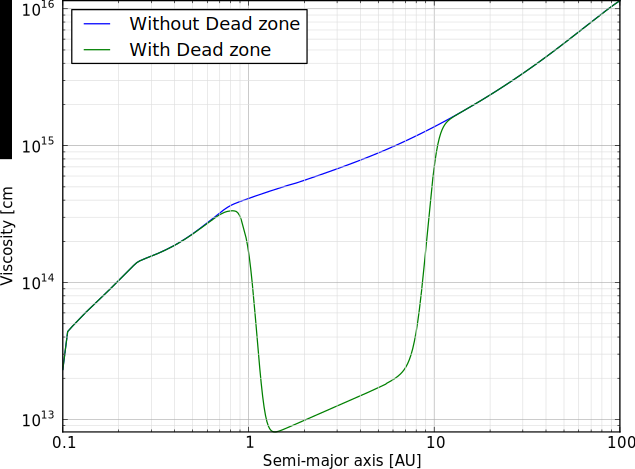
\includegraphics[width=0.6\linewidth]{figure/migration_map/viscosity/dead_zone_profile.pdf}
\caption{Profils de viscosité du disque selon qu'une zone morte est modélisée ou pas. En dehors de la zone morte $\alpha=5\cdot 10^{-3}$. Dans la zone morte, $\alpha=10^{-4}$. Ces profils correspondent à chacune des deux cartes de migration
présentées \protect\reffig{fig:viscosity_DZ}. \refdisk}\label{fig:dead_zone_profile}
\end{figure}

Dans la zone morte, la viscosité chute rapidement, et augmente en fonction de la distance dans un régime différent que dans le reste du disque \reffig{fig:dead_zone_profile}. 

\begin{figure}[htb]
\centering
\subfloat[Sans dead zone]{\includegraphics[width=0.49\textwidth]{figure/migration_map/viscosity/alpha_5e-3.pdf}}\hfill
\subfloat[Avec dead zone]{\includegraphics[width=0.49\textwidth]{%
figure/migration_map/viscosity/alpha_dz.pdf}}

\caption{Effet d'une zone morte sur la carte de migration. Au cœur de la dead zone, $\alpha=10^{-4}$. En dehors, $\alpha=5\cdot 10^{-3}$. Dans les zones de transitions, la valeur de $\alpha$ est lissée. La zone morte s'étend de $1$ à $10\unit{UA}$. Plus de détails sur la modélisation de la zone morte \protect\refsec{sec:dead_zone}. \refdisk}\label{fig:viscosity_DZ}
\end{figure}

Sur les cartes de migration \reffig{fig:viscosity_DZ}, l'entrée dans la dead-zone modifie en profondeur la carte de migration en creusant une zone de migration vers l'intérieur en raison de la viscosité très faible. Le temps de diffusion visqueux $t_\text{visc}$ augmente alors brusquement, engendrant la saturation rapide du couple de corotation quelle que soit la masse de la planète. Ainsi, dans la zone morte, la possibilité de migration vers l'extérieur est fortement réduite. En dehors de la zone morte, la carte de migration est quasi inchangée. 

\section{Effets des paramètres du disque}
%TODO see kretke2012importance
%TODO regarder le papier de Bitsch 2013 et celui de 2012 où il regarde l'influence de l'indice adiabatique
%TODO essayer des gammes beaucoup plus larges de paramètres

Jusqu'à présent, je me suis concentré sur des cas particuliers. Dans le cas de la formation de super-Terres, je n'ai considéré
qu'un seul disque \refsec{sec:4.2}. Dans le cas du décalage de la zone de convergence, j'ai montré un disque artificiel
modélisant une zone de convergence \refsec{sec:shifted_CZ}. 

Je vais montrer dans les paragraphes qui suivent que la migration est extrêmement sensible aux paramètres du disque.

\cite{kretke2012importance} ont étudié l'influence des paramètres du disque sur la migration. Cependant, s'ils ont inclus des
effets fins sur le bord interne et la migration, la dépendance de l'opacité en fonction de la température et de la densité est
approximée par différentes lois de puissance. Nous montrerons que l'opacité est un paramètre sensible du modèle et qu'il est
important de la modéliser le plus finement possible. 

\cite{bitsch2013influence} ont étudié en particulier l'effet de la viscosité $\nu$ et l'indice adiabatique $\gamma$ sur la
migration dans le disque, au travers de simulations 3D. 

Afin d'étudier séparément l'effet des paramètres du disque, j'ai choisi un disque de référence, décrit
\refsec{sec:migrations-maps}. Dans cette section je présente les cartes de migration et comment les interpréter. En particulier
je présente la carte de migration du disque de référence \reffig{fig:fiducial_migration_map}. Pour chaque paramètre, je vais
donc conserver les valeurs du disque fiducial, et faire varier le paramètre en question autour de la valeur de référence. Sauf
mention contraire, un seul paramètre est donc modifié à la fois, seuls les paramètres qui changent sont précisés, les autres
sont regroupés \reftab{tab:fiducial_parameters}.

%TODO continuer

%TODO 

\subsection{Effet de l'irradiation}
En choisissant ou non d'inclure l'irradiation dans l'équation de l'énergie permettant de calculer le profil de température, on
change de manière importante la carte de migration \citep{bitsch2013stellar}. 

%TODO dire que l'irradiation transforme la zone dépendante de la masse en zone indépendante de la masse
%TODO faire référence à hasegawa et pudritz 2011. Dnas leur papier ils font référence à un piège à planète au moment de la
%transition disque actif/passif

\begin{figure}[htb]
\centering
\subfloat[Avec irradiation]{\includegraphics[width=0.49\textwidth]{figure/migration_map/bell_irr.pdf}}\hfill
\subfloat[Sans irradiation]{\includegraphics[width=0.49\textwidth]{%
figure/migration_map/bell_noirr.pdf}}

\caption{Influence de l'irradiation sur la carte de migration à travers le profil de température. Afin de visualiser plus
facilement les effets, \cite{bell1994FU} a été utilisé pour l'opacité. \refdisk}\label{fig:irradiation}
\end{figure}

Afin de visualiser l'effet de l'irradiation, nous avons utilisé les lois d'opacités de \cite{bell1994FU}. En effet,
le principal effet de l'irradiation est de lisser le profil de température. Sans irradiation, une transition d'opacité marquée
comme celles de \cite{bell1994FU} se répercute directement sur le profil de température \reffig{fig:temp_profile_irradiation}.
On voit donc apparaître des zone de convergences dues à des transitions d'opacités qui sont déformées par
l'irradiation comme on peut le constater sur \reffig{fig:irradiation}.

\begin{figure}[htb]
\centering
\includegraphics[width=0.6\linewidth]{figure/migration_map/temperature_with_irradiation.pdf}
\caption{Profil de température avec ou sans irradiation. \refdisk}\label{fig:temp_profile_irradiation}
\end{figure}

Ainsi, sans irradiation, les deux transitions d'opacités à $1.3$ et $2.9\unit{UA}$ induisent un changement brutal de la pente
du profil de température, ce qui a pour effet de changer le sens de migration (de positif à négatif, puis l'inverse).

Dans les parties externes, l'irradiation a pour effet de diminuer la pente du profil de température qui tend vers un profil en
$R^{-0.5}$ quand le disque est purement passif.

%TODO expliquer pourquoi les parties externes ``montent'' en masse. En clair, au lieu d'avoir une décroissance de la zone de
% couple nul avec la masse, c'est l'inverse qui se produit quand on active l'irradiation.



\subsection{Masse du disque}
%TODO discuter la dissipation plus en détail, en particulier reprendre la partie dissipation phtooévaporation du début, et
%discuter de ce qu'il pourrait se passer au niveau de la migration par rapport à ce que j'ai extrait des effets du disque.
\begin{figure}[htb]
\centering
\subfloat[$\Sigma_0=400\unit{g/cm^2}$]{\label{fig:map_low_mass}\includegraphics[width=0.49\textwidth]{%
figure/migration_map/total_mass/high_mass.pdf}}\hfill
\subfloat[$\Sigma_0=200\unit{g/cm^2}$]{\label{fig:map_high_mass}\includegraphics[width=0.49\textwidth]{%
figure/migration_map/total_mass/low_mass.pdf}}

\caption{Par rapport au disque de référence, possédant un profil de densité de surface $\Sigma(R) = 300 \cdot
R^{-\sfrac{1}{2}}\unit{g/cm^2}$ nous représentons la carte de migration dans un cas un peu moins et un peu plus massif, avec le
même indice de la loi de puissance. Les échelles ne sont pas les mêmes, elles ont été choisies pour montrer que la forme reste
globalement conservée, si on s'affranchit de l'échelle absolue de la taille de cette dernière.
\refdisk}\label{fig:map_total_mass}
\end{figure}

Dissiper le disque par une exponentielle décroissante signifie changer la masse du disque au cours du temps sans modifier
son profil de densité de surface.

Pendant la dissipation, la zone de convergence externe va peu à peu se déplacer vers l'intérieur du disque. À mesure que la masse diminue, le chauffage visqueux diminue aussi. La température diminue alors. Même si c'est l'irradiation qui domine dans les parties externes, la diminution du chauffage visqueux influe sur la position de la zone de couple nul. La zone de
convergence externe qui était à $20\unit{UA}$ environ pour des planètes dont la masse est comprise entre $15$ et $40\mearth$
\reffig{fig:map_high_mass} va se retrouver à $10\unit{UA}$ environ avec un disque moins massif \reffig{fig:map_low_mass}. 

À partir de la carte de migration d'un disque donné nous pouvons définir la masse critique supérieure (resp. inférieur) au
dessus (resp. en dessous) de laquelle on a systématiquement migration vers l'intérieur des planètes, quelle que soit leur
position. À mesure que le disque se dissipe,  les masses critiques diminuent. Ainsi, les planètes entre $30$ et $45\mearth$ qui
pouvaient auparavant migrer vers l'extérieur dans certaines zones du disque \reffig{fig:map_high_mass} ne peuvent plus le faire
dans un disque un peu moins massif \reffig{fig:map_low_mass}. Les planètes entre $3$ et $5\mearth$ qui ne pouvaient que migrer
vers l'intérieur \reffig{fig:map_high_mass} peuvent maintenant migrer vers l'extérieur dans certaines zones du disque moins
massif \reffig{fig:map_low_mass}. 

Étudier l'influence de la masse du disque nous permet de remonter à l'effet de la dissipation du disque. En particulier dans la première phase de la dissipation, quand le profil de densité de surface n'évolue pas beaucoup. Dans la seconde partie gouvernée par la photo-évaporation, la dissipation ne conserve pas le profil en loi de puissance de la densité de surface (en faisant que ce dernier en est un initialement) \reffig{fig:disk_dispersion}. Au lieu de ça, le
disque va se creuser à partir d'un certain rayon, optimal vis à vis de la photo-évaporation. Le disque va alors se scinder en
deux, la partie interne va rapidement tomber sur l'étoile centrale et dans un dernier stade les parties externes vont aussi se
dissiper. Si les détails de la dissipation ne sont pas connus, il apparait malgré tout qu'une unique décroissance exponentielle du disque tout au long de sa vie ne représente pas fidèlement l'évolution du disque. Dans le cadre de la migration planétaire où les profils de densité et de températures jouent un rôle fondamental, nous nous limitons donc à l'étude des premiers millions d'années d'évolution du disque. 

La dispersion du disque a été discutée brièvement \refsec{sec:dispersion}.

\subsection{Profil de densité de surface}
Dans notre modèle, le profil de la densité de surface est notre plus grande incertitude. Les contraintes observationnelles ne
restreignent pas suffisamment le profil de densité \citep[Fig. 12]{guilloteau2011dual}. Il y a peu de chance que la densité de
surface d'un disque réel puisse être défini par une loi de puissance d'un bout à l'autre, et surtout par la même loi de
puissance. 

On définit la loi de puissance pour la densité de surface de la façon suivante : 
\begin{align}
\Sigma(R) &= \Sigma_0 * \left(\frac{R}{R_0}\right)^{-d}
\end{align}
où $\Sigma_0$ est la densité de surface à $R_0=1\unit{UA}$.

Je cherche à étudier l'influence de l'indice $d$ de la loi de puissance sur la carte de migration. Je vais me concentrer sur
deux cas particuliers. Dans le premier cas, je vais étudier la variation de l'indice sans changer $\Sigma_0$, c'est à dire que
la masse totale du disque va varier en même temps que l'indice. Dans un deuxième cas, la masse totale du disque entre $0.1$ et
$100\unit{UA}$ est constante, et on varie la densité de surface à $1\unit{UA}$, $\Sigma_0$ en même temps que l'indice $d$ de la
loi de puissance.

\begin{figure}[htb]
\centering
\subfloat[$d=0.6$ ; $\Sigma_0=300\unit{g/cm^2}$]{\label{fig:d06}\includegraphics[width=0.49\textwidth]{%
figure/migration_map/index/300_06.pdf}}\hfill
\subfloat[$d=0.7$ ;
$\Sigma_0=300\unit{g/cm^2}$]{\label{fig:d07}\includegraphics[width=0.49\textwidth]{figure/migration_map/index/300_07.pdf}}

\caption{Influence de l'indice $d$ de la loi de puissance définissant la densité de surface du disque sur la carte de migration.
Ici, $\Sigma_0=\cte=300\unit{g/cm^2}$, seul l'indice du profil de densité de surface varie. \refdisk}\label{fig:map_index}
\end{figure}

Si l'indice $d$ du profil de densité de surface augmente, la forme de la carte de migration aura tendance à se compresser vers
les parties internes du disque. En effet, en dessous de $R_0=1\unit{UA}$ la densité de surface sera plus importante si $d$
augmente. Mais dans les parties externes, au delà de $R_0=1\unit{UA}$ la densité de surface sera plus faible. La température
dans ces régions là sera alors plus faible. La diffusivité thermique $\chi$ étant extrêmement sensible à la température, si $T$
diminue cela entraine la diminution de $\chi$. Le temps de diffusion radiatif $t_\text{rad}$ étant inversement proportionnel à
la diffusivité thermique $\chi$, si l'indice du profil de densité de surface augmente, le temps de diffusion radiatif augmente.
En fonction de la distance, le couple de corotation sature ainsi plus rapidement. L'augmentation de $d$ dans
\reffig{fig:map_index} illustre cet aspect. 

On peut remarquer que l'augmentation de l'indice du profil de densité de surface va avoir un impact sur la masse totale du
disque. On a vu précédemment que la masse totale du disque avait un effet inverse par rapport à l'indice $d$. Si on augmente
l'indice $d$, on compresse la zone de migration externe vers l'étoile centrale. Au contraire, si on augmente la masse totale, on
dilate cette zone radialement. 

\begin{figure}[htb]
\centering
\subfloat[$d=0.6$ ; $\Sigma_0=444\unit{g/cm^2}$]{\label{fig:d06iso}\includegraphics[width=0.49\textwidth]{%
figure/migration_map/index/444_06.pdf}}\hfill
\subfloat[$d=0.7$ ;
$\Sigma_0=653\unit{g/cm^2}$]{\label{fig:d07iso}\includegraphics[width=0.49\textwidth]{figure/migration_map/index/653_07.pdf}}

\caption{Influence de l'indice $d$ du profil de densité de surface tout en maintenant la masse totale du disque constante.
\refdisk}\label{fig:map_index_mtot}
\end{figure}

On constate sur \reffig{fig:map_index_mtot} que dans ce cas là, l'étendue spatiale de la zone de migration vers l'extérieur
reste équivalente. On remarque cependant des variations complexes dans les parties internes du disques, difficiles à attribuer à
un seul effet isolé. 

Néanmoins, de cette analyse on remarque qu'à masse constante du disque, la migration est similaire d'un disque à l'autre dans
les parties externes où les différences de densité sont très faibles localement. Seules les parties internes présentent des
différences notables de densité. Ceci s'explique par le fait que dans mon cas, j'ai tenu à maintenir une masse constante dans la
totalité du disque, c'est à dire de $0.1$ à $100\unit{UA}$. 

\bigskip

Un examen détaillé de ces cartes de migration nous montre ainsi deux choses. Premièrement que la zone de migration vers
l'extérieur est tronquée dans les parties externes à mesure que le gradient de densité de surface augmente. Cet effet s'oppose à
la tendance inverse qui est observée quand on augmente la densité de surface locale (ce qui augmente la température, puis la
diffusivité thermique). 

Deuxièmement, en conservant une densité locale sensiblement égale comme c'est le cas entre $6$ et $18\unit{UA}$ pour les disques
\reffig{fig:map_index_mtot} on conserve aussi la carte de migration. Cependant, la sensibilité très forte aux transitions
d'opacité et au profil de température rendent difficile l'interprétation des parties internes du disque. 


%TODO 
\subsection{Table d'opacité}\label{sec:influence_opacity_table}
Le modèle utilisé pour déterminer les opacités dans un disque est bien souvent à peine nommé, et très peu discuté. Pourtant,
l'opacité est une grandeur physique qui a une influence très importante sur la physique du disque et la migration des planètes. 

Dans toute la suite, quand je parlerai de table d'opacité, je désigne le fait d'utiliser un tableau à deux dimensions,
proposant des valeurs de l'opacité pour différentes températures et densités. La table d'opacité est donc définie ici par
opposition à ce que j'appelle des lois d'opacité, modèles dans lesquels l'opacité est définie par des lois de puissance,
fonction de la température et de la densité, dans différents régimes de température et densité.

Ainsi une table d'opacité est simplement une tabulation de l'opacité, alors qu'une loi d'opacité correspond à un ajustement par
une loi de puissance. 

\bigskip

Généralement, c'est la loi d'opacité \cite{bell1994FU} qui est utilisée, aussi bien dans les simulations hydrodynamiques 2D et
3D que dans les simulations N-corps. 

Une autre loi d'opacité existante est \cite{zhu2009nonsteady}, loi quelque peu améliorée par rapport à \cite{bell1994FU},
l'augmentation des capacités des ordinateurs ayant permis de faire des calculs plus précis. 

De plus, nous utilisons aussi le modèle d'opacité très simple décrit par \cite{chambers2009analytic} dans lequel l'opacité est
constante et égale à $\kappa=3$ jusqu'à $1380\unit{K}$ où une transition s'opère vers une loi de puissance. Ce modèle nous
permet de voir l'effet d'un modèle par rapport à un cas où l'opacité est constante. En effet, dans le cas d'un disque
protoplanétaire, seules les régions les plus internes sont susceptibles d'atteindre des températures supérieures à
$1000\unit{K}$. 

Enfin, j'ai souhaité comparer ces deux lois d'opacité avec une table d'opacité, \cite{hure2000transition}. Cette table
d'opacité de Rosseland correspond à la composition suivante $X=0.70$, $Y=0.28$ et $Z=0.02$ et est basée sur
\cite{seaton1994opacities, alexander1994low, henning1996dust}.

\begin{figure}[htb]
\centering
\subfloat[\citep{bell1994FU}]{\includegraphics[width=0.49\textwidth]{figure/migration_map/opacity/opacity_bell.pdf}}\hfill
\subfloat[\citep{chambers2009analytic}]{\includegraphics[width=0.49\textwidth]{%
figure/migration_map/opacity/opacity_chambers.pdf}}

\subfloat[\citep{zhu2009nonsteady}]{\includegraphics[width=0.49\textwidth]{figure/migration_map/opacity/opacity_zhu.pdf}}\hfill
\subfloat[\citep{hure2000transition}]{\label{fig:opacity_hure}\includegraphics[width=0.49\textwidth]{%
figure/migration_map/opacity/opacity_hure.pdf}}
\caption{Cartes de migration obtenues pour le même disque, mais avec un modèle d'opacité différent. L'irradiation ayant un
effet important sur la carte de migration, elle a été désactivée ici afin de mieux mettre en valeur les différences entre
les modèles d'opacités. Notez que les échelles ne sont pas identiques. \refdisk}
\end{figure}\label{fig:opacity_tables}

\reffig{fig:opacity_tables} montre les différentes cartes de migration que l'on obtient avec le même disque de référence mais
pour les 4 modèles d'opacité considérés. 

On considère la carte avec la table d'opacité \reffig{fig:opacity_hure} comme référence. En effet, les lois d'opacités utilisent
une table d'opacité en amont à partir de laquelle elles déduisent des lois de puissances par morceau afin de reproduire au mieux
la table d'opacité. La table d'opacité se traduit par une carte de migration complexe où chaque aspect de la table se traduit
sur la carte par une variation brutale de la migration. L'opacité a une grande influence sur la migration, que ce soit au
niveau du temps de diffusion qui régi la saturation que vis à vis du profil de température.

L'importance de l'opacité se manifeste au travers du temps de diffusion radiatif. Une opacité plus grande induit un temps de
diffusion radiatif plus important. 

On constate par ailleurs que les lois d'opacité lissent fortement la carte de migration (comparer la carte pour la table
d'opacité d'\cite{hure2000transition} avec les 3 autres). Notons en particulier une transition d'opacité dans \cite{bell1994FU}
qui n'existe pas dans les autres modèles et qui entraine une zone de convergence indépendante de la masse (dans le cas présent
à $1.3\unit{UA}$). Cette transition d'opacité, liée à l'évaporation des grains de glace d'eau, n'est en effet introduite que
dans ce modèle, les autres modèles considérant qu'elle n'illustre aucune réalité physique 
%TODO Ref sur la transition d'opacité fantome

Le modèle d'opacité choisi a donc une grande influence sur la carte de migration et donc le comportement des planètes dans un
disque. À l'heure actuelle, compte tenu de la puissance des ordinateurs, le choix d'une loi d'opacité par rapport à une table
d'opacité ne se justifie plus. En effet, les approximations supplémentaires qu'engendrent une loi d'opacité comparé
à une table brute ne sont pas compensées par le gain de temps de calcul que cela engendre. Dans mon cas, la routine
implémentant la table d'opacité est même plus rapide que la routine pour les lois d'opacités. La seule différence est qu'il
faut stocker un tableau contenant la table d'opacité, ce qui n'est pas limitatif avec les ordinateurs actuels.

Les modèles d'opacités étant une source d'incertitude pour toutes les simulations numériques, que ce soit des simulations
N-corps ou des simulations hydrodynamiques 2D ou 3D, je pense qu'il est important d'apporter une attention particulière au
choix du modèle. 

À l'heure actuelle, dans le cas particulier de la migration planétaire, la valeur de l'opacité ainsi que la pente qu'elle
engendre sur le profil de température sont des sources importantes d'incertitudes. Il pourrait être intéressant de réaliser une
étude d'envergure afin de réaliser une table d'opacité tenant compte des nouvelles capacités des ordinateurs, afin de coller au
mieux à ce que l'on sait des disques. 

Il restera pourtant toujours des incertitudes quant aux propriétés des poussières, taille et quantité, ainsi que son évolution
au cours du temps. La poussière étant une source majeure d'opacité dans le disque, son évolution au cours du temps doit avoir
une influence toute aussi majeure que nous ne pouvons que négliger à l'heure actuelle malgré les implications que cela peut
avoir sur la formation des planètes.

%TODO

\subsection{Longueur de lissage}
Dans les modèles numériques des disques protoplanétaires, le potentiel gravitationnel doit être modifié afin ne pas diverger aux
très faibles distances mutuelles. En particulier, des problèmes peuvent survenir quand on modélise des objets étendus par des
masses ponctuelles. Le modèle de Plummer introduit une longueur de lissage $b$ (souvent notée $b/h$ car sa valeur est exprimée
en fonction de l'échelle de hauteur du disque). la force de gravitation adoucie s'écrit alors : 
\begin{align}
\vect{F_{ij}} &= G m_i m_j \frac{\abs{r_i - r_j}}{\left(\abs{r_i - r_j}^2 + b^2\right)^\sfrac{3}{2}}
\end{align}


De même, dans le cas de simulations hydrodynamiques 2D, le modèle se base sur des moyennes verticales des différentes quantités
physiques. Le lissage du potentiel gravitationnel est ici nécessaire afin de diluer le potentiel et reproduire au mieux l'aspect
3D du disque. On comprend alors aisément que la longueur de lissage va être reliée à l'échelle de hauteur du disque qui est elle
aussi une mesure de l'extension verticale du disque. 

Plusieurs groupes ont cherché à étudier la longueur de lissage en détail, en particulier pour trouver la valeur optimale à
utiliser \citep{hure2009local, muller2012treating}. Ces études cherchent à trouver la longueur de lissage qui permet de
reproduire les simulations 3D à l'aide des simulations 2D. 

Une longueur de lissage relativement importante $b/h = 0.75$ est nécessaire pour reproduire correctement le couple de Lindblad
\citep{masset2002coorbital}. Pour le couple de corotation, la zone fer-à-cheval étant très proche de la planète, ce dernier est
extrêmement sensible à la longueur de lissage. En effet, \cite{masset2002coorbital} a montré que dans certains cas le couple de
corotation pouvait être plus d'un ordre de grandeur plus important en fonction de la valeur du lissage que l'on applique. La
valeur préconisée est alors autour de $b/h\sim 0.5-0.6$. Ainsi, \cite{masset2002coorbital} conclue qu'il est peu probable de
trouver une valeur optimale pour la longueur de lissage, les valeurs optimales pour les couples de Lindblad et de corotation
étant incompatibles. 

\cite{muller2012treating} suggère d'utiliser une longueur de lissage $b/h = 0.7$ tout en notant que des différences notables
subsistent avec les simulations 3D. 

\cite{hure2009local}, en étudiant des disques sans planètes conseillent la plage de valeur suivante $0.13 \lesssim b/h \lesssim
0.29$.

\bigskip

\cite{paardekooper2010torque, paardekooper2011torque} et les formules analytiques ou semi-analytiques qu'ils fournissent pour
décrire la migration de type I (\refeq{eq:lindblad-torque}, \refeq{eq:saturated-corotation-torque},
\refeq{eq:linear-corotation-torque}) introduisent une telle dépendance. 

\begin{figure}[htb]
\centering
\subfloat[$b/h = 0.2$]{\includegraphics[width=0.49\textwidth]{figure/migration_map/smoothing/smoothing_0_2.pdf}}\hfill
\subfloat[$b/h = 0.4$]{\includegraphics[width=0.49\textwidth]{figure/migration_map/smoothing/smoothing_0_4.pdf}}\\
\subfloat[$b/h = 0.6$]{\includegraphics[width=0.49\textwidth]{figure/migration_map/smoothing/smoothing_0_6.pdf}}\hfill
\subfloat[$b/h = 0.7$]{\includegraphics[width=0.49\textwidth]{figure/migration_map/smoothing/smoothing_0_7.pdf}}\\
\caption{Effet de la longueur de lissage $b/h$ du potentiel gravitationnel sur la carte de migration du disque de référence.
\refdisk}\label{fig:migration_map_smoothing}
\end{figure}

\reffig{fig:migration_map_smoothing} montre qu'en fonction de la longueur de lissage, on peut se trouver dans un cas où il y a
migration systématique vers l'intérieur ($b/h=0.7$) ou migration quasi systématique vers l'extérieur ($b/h=0.2$). Si une valeur
de $0.2$ semble peu réaliste au regard de la migration planétaire \citep{muller2012treating}, il est courant de voir des
simulations effectuées avec $b/h=0.3-0.6$ \citep{masset2002coorbital, devalborro2006comparative, paardekooper2009corotation}. 

Une longueur de lissage $0.6 \leqslant b/h \leqslant 0.76$ sous estime le couple de corotation et sur-estime le couple de
Lindblad \citep{masset2002coorbital}. Même si les valeurs préconisées par les études de sensibilités se situent autour de
$0.6-0.7$, les études faisant des simulations hydrodynamiques utilisent plus couramment une valeur de $b/h=0.4$
\citep{paardekooper2011torque}. Il n'existe donc pas de valeur optimale pour la longueur de lissage quand le disque que l'on
modélise est utilisé pour étudier la migration planétaire. Si cette section ne conclue pas quant à une valeur à utiliser pour
$b/h$ c'est avant tout pour insister sur le fait que la seule conclusion à tirer, c'est que la longueur de lissage est une
source importance d'incertitude dans nos modèles. Une longueur de lissage importante (resp. faible) a tendance à favoriser la
migration vers l'intérieur (resp. l'extérieur). 

\begin{figure}[htb]
\centering
\subfloat[$b/h = 0.5$]{\includegraphics[width=0.49\textwidth]{figure/migration_map/smoothing/smoothing_0_5.pdf}}\hfill
\subfloat[$b/h = 0.76$ pour $\Gamma_L$ et $0.5$ pour
$\Gamma_C$]{\includegraphics[width=0.49\textwidth]{figure/migration_map/smoothing/smoothing_0_5_modified.pdf}}
\caption{Comparaison d'un cas où la longueur de lissage est fixée à $b/h=0.5$, et d'un autre cas où la longueur de lissage a été
fixée à $0.76$ pour le couple de Lindblad et à $0.5$ pour le couple de Corotation, correspondant aux valeurs conseillées pour
les deux couples séparés \citep{masset2002coorbital}. \refdisk}\label{fig:modified_smoothing}
\end{figure}

Inclure des formules pour la migration de type I nous offre une liberté supplémentaire par rapport aux simulations
hydrodynamique, celle de fixer une longueur de lissage $b/h$ différente pour le couple de Lindblad et pour le couple de
Corotation. Suivant les prescriptions données par \cite{masset2002coorbital} j'ai donc calculé la carte de migration d'une
simulation où je fixe une longueur de lissage $b/h=0.76$ pour le couple de Lindblad, et une longueur de lissage $b/h=0.5$ pour
le couple de Corotation. J'obtiens alors les cartes représentées \reffig{fig:modified_smoothing}, toujours dans le cas du disque
de référence. %TODO décrire le disque de référence en section 3, et en particulier penser à emttre une référence ici vers la
bonne section.

%TODO proposer cette idée d'utiliser une longueur de lissage différente pour lindblad et corotation? En discuter avec Sean et
%Arnaud.


%TODO parler du travail d'audrey? Je voudrais en parler avec elle, lui montrer cette section et savoir ce qu'elle en pense. 
% En particulier, j'aimerais discuter avec elle du fait que la longueur de lissage qu'elle calcule ne peut pas s'appliquer dans
%mon cas à moi. J'aimerais voir si elle saurait m'expliquer pourquoi (dans mon cas j'ai une planète, et pas elle)

\subsection{Masse moléculaire moyenne}
La masse moléculaire moyenne $\mu$ va varier dans le disque, principalement à cause de l'évaporation de certaines
espèces chimiques à différentes températures. La plupart sont négligeable vu leur abondance limitée. Le problème
aurait pu se poser au bord interne du disque, où la température est très importante. Dans cette région là, la masse moléculaire
moyenne peut varier à cause de la photodissociation de la molécule $\mathrm{H_2}$. En supposant que le rapport d'abondance
$\mathrm{He/H}=0.1$, la masse moléculaire, initialement de $\mu=2.35$ passe alors à environ $\mu\sim 1.3$ \citep[Annexe
A]{hure2000transition}.

\begin{figure}[htb]
\centering
\subfloat[$\mu=2.35$]{\includegraphics[width=0.49\textwidth]{figure/migration_map/mmw_fully_molecular.pdf}}\hfill
\subfloat[$\mu=1.3$]{\includegraphics[width=0.49\textwidth]{figure/migration_map/mmw_HI.pdf}}
\caption{Influence de la masse moléculaire moyenne $\mu$ sur la carte de migration. Seules les
parties très internes du disque sont ici représentées. Le même disque est utilisé, seule la masse
moléculaire change afin de refléter l'influence de la photodissociation de $\mathrm{H_2}$ en
$\mathrm{HI}$ quand la température devient importante. \refdisk}\label{fig:migration_map_mmw}
\end{figure}

\reffig{fig:migration_map_mmw} montre l'influence de la masse moléculaire moyenne sur la carte de migration pour un disque
donné. On s'attend à ce que la photodissociation de $\mathrm{H_2}$ ne devienne importante que dans les parties très internes,
bien en dessous de $1\unit{UA}$. Dans ces régions là, on constate que la variation de la masse moléculaire moyenne n'a que peu
d'effet. Il ne nous est donc pas apparu important de prendre cette variation en compte, les changements induits sur la carte de
migration étant bien inférieur à l'influence du modèle d'opacité par exemple. Cet effet nous parait donc négligeable au regard
des incertitudes de notre modèle.


\chapter{Mécanismes de formation}\label{sec:chap4}\index{super-Terre}\index{noyau de planète géante}

\section{Décalage de la Zone de Convergence}\label{sec:shifted_CZ}
Cette partie a fait l'objet d'un article, publié dans le journal Astronomy \& Astrophysics : \cite{cossou2013convergence}.

Une zone de convergence est une zone du disque agissant comme un piège à planète, la migration emmenant les planètes dans cette zone du disque où elles se stabilisent. Ici nous cherchons à montrer que dans le cas multi planétaire, les choses sont un peu différentes. Des planètes en résonance ne se comportent plus de la même manière, mais plutôt comme un système dans sa globalité, migrant dans une zone différente du disque.

\subsection{Introduction}
Des planètes de faible masse ($1-60\mearth$) interagissent avec le disque de gaz dans lequel elles se forment et génèrent des ondes de densité dans le disque \citep{goldreich1979excitation}. La planète elle même est influencée par cette onde de densité et migre par migration de Type I \citep{ward1997protoplanet}.

Dans les disques isothermes, la migration de Type I est gouvernée par le couple différentiel dû aux ondes de Lindblad et le couple de corotation. Pour les planètes, la migration qui en résulte est rapide et dirigée vers l'étoile centrale \citep{tanaka2002three}. Dans les disques radiatifs, un couple lié au gradient d'entropie apparait dans la zone en fer-à-cheval de la planète. Ce dernier peut contrebalancer le couple différentiel de Lindblad au point de transformer la migration vers l'intérieur précédemment présentée en migration vers l'extérieur. Ainsi, dans de tels disques, la migration peut être dirigée soit vers l'intérieur soit vers l'extérieur \citep{paardekooper2006halting, kley2008migration}. Ceci rend possible l'existence de zones dans les disques où la migration s'arrête. Ces dernières sont appelées zone de convergence \citep[CZs;][]{lyra2010orbital, mordasini2011application, paardekooper2011torque}.

\bigskip

À la zone de convergence, le couple de corotation (positif) compense exactement le couple différentiel de Lindblad (négatif). Ainsi, à la zone de convergence, une planète ne migre pas. Les zones de convergences pourraient ainsi concentrer les embryons planétaires et être le lieu de formation de planètes (ou cœurs) massives \citep{lyra2010orbital, horn2012orbital}. 

Cependant, durant leur migration vers la zone de convergence les planètes vont interagir entre elles et se placer en résonance de moyen mouvement (Mean Motion Resonance : MMR), s'opposant ainsi à l'accrétion illimitée de matière à la zone de convergence \citep{morbidelli2008building, sandor2011formation}. Malgré cela, des collisions ont bien lieu à la zone de convergence. Quand les embryons sont emprisonnés dans une chaine de résonance avec suffisamment de corps pour engendrer des perturbations, les résonances peuvent se briser et des collisions se produire entre les corps du système. De plus, la turbulence pourrait casser les résonances et augmenter le taux d'accrétion.

\bigskip

\cite{bitsch2010orbital} ont montré que le couple de corotation était atténué quand une planète avait une excentricité telle que son orbite oscille sur une distance de l'ordre de la demi-largeur de la zone fer-à-cheval $x_s$. 

Quand deux planètes sont en résonance à cause de la migration convergente, leurs excentricités sont excitées de manière continues malgré la présence du disque qui a tendance à amortir les excentricités et circulariser les orbites. \citep[par exemple ][]{cresswell2008three}. Ce phénomène devrait à son tour modifier le couple de corotation et ainsi modifier l'équilibre entre couple différentiel de Lindblad et couple de corotation. En conséquence, la migration de la planète elle-même devrait être modifiée.

\bigskip

Nous présentons des simulations de migration convergentes de planètes de faible masse ($M=1-10\unit{M_\oplus}$) dans un disque de gaz idéalisé (voir \refsec{sec:tanh_indep}). On utilise un modèle simplifié de rétroaction de l'excentricité sur le couple de corotation. Nous montrons que les planètes qui prises de manière isolé migrent à la zone de convergence, ne migrent plus au même endroit quand il y a plusieurs planètes. Au lieu de ça, elles migrent à une position d'équilibre décalée vers l'intérieur du disque qui correspond à une somme nulle des couples exercées sur le système. 

La position de cette zone d'équilibre dépend de l'excentricité maintenue par perturbation mutuelle de chaque planète constituante du système.

\subsection{Méthode}
On modélise une Zone de Convergence (CZ : Convergence Zone) artificielle, qui imite une zone de convergence indépendante de la masse, c'est à dire que la position de la zone de convergence est la même pour toutes les planètes quelle que soit leur masse \refsec{sec:CZ-types}. En particulier, on s'intéresse à la zone de convergence que l'on peut trouver à une transition d'opacité telle que celle représentée sur \reffig{fig:shifted_CZ_torque_prof}, où l'on peut voir un renversement brutal du couple, qui passe de positif à négatif \citep[voir par exemple ][]{masset2011type}.

\begin{figure}[htb]
\centering
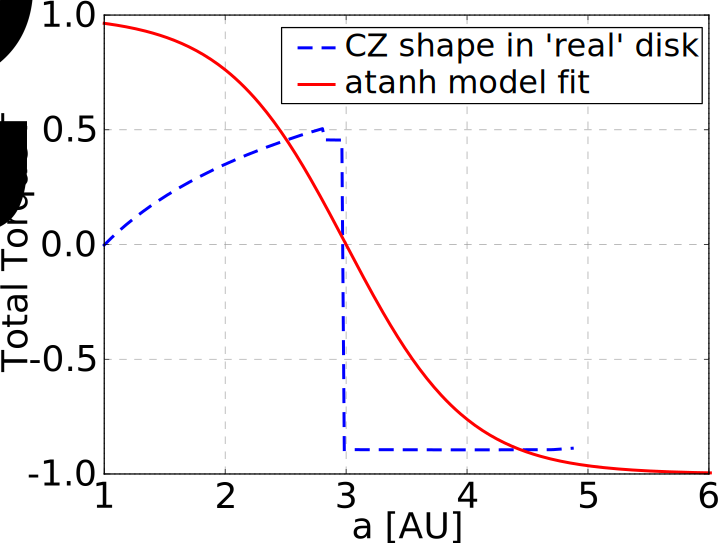
\includegraphics[width=0.49\linewidth]{figure/shifted/torque_zoom_CZ1.pdf}
\caption{Le couple total de notre disque standard est représenté en rouge. La ligne bleue pointillée représente le profil de couple ressenti par une planète de $10\unit{M_\oplus}$ autour d'une transition d'opacité, calculé à partir des équations de \cite{paardekooper2011torque}.}\label{fig:shifted_CZ_torque_prof}
\end{figure}

À noter qu'une fonction de Heavyside n'a pas été utilisée car la marche d'escalier dans le profil \textit{réel} n'est due qu'au fait que la table d'opacité n'a pas été lissée. On s'attend à ce que la transition soit plus douce dans la réalité.
%TODO arnaud veut que je compare une version lissée avec mon tangente hyperbolique.

La position de la zone de convergence était $3\unit{UA}$. À l'intérieur de $3\unit{UA}$, le couple est positif et égal à $\Gamma_0 = \left(\frac{q}{h}\right)^2\Sigma_p {r_p}^4 {\Omega_p}^2$., la migration se fait donc vers l'extérieur. Au delà de $3\unit{UA}$, le couple total est égal à $-\Gamma_0$. Ici $q$ est le rapport entre les masses de la planète et de l'étoile, $h$ est le rapport d'aspect qui dépend du profil de température mais vaut typiquement $0.05$. $\Sigma_p$, $r_p$ et $\Omega_p$ sont respectivement la densité de surface, la distance orbitale et la vitesse angulaire pour la planète. 

Le couple total est la somme du couple différentiel de Lindblad $\Gamma_L$ --- que l'on suppose constant et indépendant de $e$ --- et le couple de corotation $\Gamma_C$. Le principal intérêt de la zone de convergence artificielle est de s'affranchir de la forme très complexe du profil réel et ne garder que la zone de convergence, afin d'en étudier les effets de manière isolée.

\bigskip

\cite{bitsch2010orbital} montrent que la structure de la zone fer-à-cheval est modifiée quand l'excentricité augmente. En conséquence, son couple de corotation $\Gamma_C$, lié à cette région du disque, diminue. 

Nous avons élaboré une formule simple qui reproduit l'effet de l'excentricité sur $\Gamma_C$ par une simple calibration des simulations 3D de \cite{bitsch2010orbital} : 
\begin{align}
D &= \frac{\Gamma_C(e)}{\Gamma_C (e=0)} = 1 + a \cdot \left[\tanh(c) - \tanh\left(\frac{b * e}{x_s}+c\right)\right]\label{eq:shifted-eccentricity-influence}
\end{align}
où $x_s$ représente la demi-largeur de la région fer-à-cheval en unité de distance orbitale de la planète considérée, $e$ est l'excentricité de la planète, et notre ajustement statistique donne les valeurs suivantes pour les paramètres de la fonction :
\begin{align}
a &= 0.45 & b &= 3.46 & c &= -2.34
\end{align}

On défini $x_s$ comme \citep[eq. (44)]{paardekooper2010torque} :
\begin{align}
x_s &= \frac{1.1}{\gamma^{1/4}} \left(\frac{0.4}{b/h}\right)^{1/4} \sqrt{\frac{q}{h}}
\end{align}
où $\gamma$ est l'indice adiabatique, $q$ le rapport entre les masses de la planète et de l'étoile, $h$ le rapport d'aspect et $b/h$ la longueur de lissage du potentiel gravitationnel de la planète (dépendance issue des formules de \cite{paardekooper2011torque}).
%TODO c'est pas uniquement un problème numérique, c'est aussi un problème physique. Voir pour cela paardekooper et papaloizou 2009 ou encore kley & muller 2012
%TODO en gros, de ce que je comprends, il y a le problème de la masse ponctuelle de la planète qui génère une divergence quand on veut calculer la forme des ondes de densité générées par la planète sur le disque. Mais il y a aussi le problème de la longueur de lissage du potentiel du disque quand on veut calculer le couple du disque sur la planète. Il y a donc techniquement deux longueurs de lissages différentes. On doit choisir une seule longueur de lissage pour le potentiel gravitationnel, mais il y a deux longueurs de lissages "optimisées" si on veut faire le calcul d'audrey, JM ou arnaud proprement ; prescription de la longueur de lissage)

\reffig{fig:shifted_CZ_D_profile} montre que notre formule simple \refeq{eq:shifted-eccentricity-influence} correspond bien à la tendance des simulations hydrodynamiques de l'effet de $e$ sur $\Gamma_C$, en particulier pour les excentricités faibles. Il faut tout de même noter qu'il y a peu de points \og expérimentaux\fg et qu'il semble y avoir des fluctuations aléatoires influençant les valeurs mesurées.

\begin{figure}[htb]
\centering
\includegraphics[width=0.49\linewidth]{figure/shifted/corotation_damping_profile.pdf}
\caption{Diminution du couple de corotation $\Gamma_C$ en fonction de l'excentricité $e$. On suppose que l'atténuation ($0<D<1$) du couple de corotation en fonction de l'extencité $e$ est la même dans un disque isotherme ou radiatif. Ainsi, on extrait la valeur de $D$ à partir de la figure 2 de \cite{bitsch2010orbital} en faisant la différence entre la valeur pour le disque radiatif et celle pour le disque isotherme, et normalisant de sorte que $D$ vale $1$ dans le cas $e=0$.}\label{fig:shifted_CZ_D_profile}
\end{figure}

\bigskip

Afin de réaliser nos simulations, nous avons utilisé la version modifiée de l'intégrateur \textbf{Mercury}\citep{chambers1999hybrid} décrite \refsec{sec:code_n-corps}. Nous avons utilisé en particulier la zone de convergence artificielle décrite \reffig{fig:shifted_CZ_torque_prof}. 

Nous supposons que le disque possède le profil de densité de surface suivant :
\begin{align}
\Sigma(R) = 500 \left(R/1\unit{AU}\right)^{-1/2} \unit{g.cm^{-2}}
\end{align}
Ce profil est alors utilisé dans le calcul de $\Gamma_0$ et de l'amortissement induit par le disque sur $e$ et $I$.

Pour implémenter la migration induite par le couple du disque $\Gamma$, on note que $\Gamma=\od{J}{t}$, et on défini une accélération de migration $a_m$ telle que\citep[eq. (14)]{cresswell2008three} :
\begin{align}
a_m &= - \frac{v}{t_m}
\end{align}
où $v$ est la vitesse de la planète et $t_m=J/\od{J}{t}$ le temps de migration ($J$ est le moment cinétique).

\bigskip

Dans toutes les simulations, les planètes était initialement sur des orbites à faible excentricité ($e<0.001$) et faible inclinaison ($I<1^\circ$). Chaque simulation a été intégrée pendant trois millions d'années, avec un pas de temps compris entre $0.4$ et $3$ jours.

\subsection{Le cas de deux planètes}
\reffig{fig:two-planets} montre l'évolution de deux planètes de $1\unit{M_\oplus}$ initialement placées de part et d'autre d'une zone de convergence située à $3\unit{UA}$. Alors qu'elles se rapprochent l'une de l'autre, les deux planètes croisent une série de résonances and finissent piégées dans la résonance \MMR{7}{6}. Les excentricités des deux planètes atteignent alors un équilibre entre excitation résonante et amortissement par le disque. Cette excentricité d'équilibre est environ égale à $0.5$ fois la demi-largeur de la zone fer-à-cheval $x_s$ et amortit le couple de corotation à environ $80\%$ de sa valeur nominale (quand $e=0$). 

\begin{figure}[htb]
\centering
\includegraphics[width=\linewidth]{figure/shifted/corotation_damping_influence.pdf}
\caption{Simulation de la migration convergence de deux planètes de $1\unit{M_\oplus}$ vers la zone de convergence située à $3\unit{UA}$, la rétroactio de l'excentricité $e$ sur le couple de corotation $\Gamma_C$ étant incluse (voir Figure~\ref{fig:shifted_CZ_D_profile}).}
\label{fig:two-planets}
\end{figure}

Les planètes se stabilisent et arrêtent de migrer à $1.77$ et $1.96\unit{UA}$, toutes les deux à l'intérieur de la position nominale de la zone de convergence. Compte tenu de leurs excentricités, la zone de convergence de la planète la plus interne est décalée à $1.95\unit{UA}$ tandis qu'elle est décalée à $1.74\unit{UA}$ pour la planète externe (située à $1.96\unit{UA}$). On constate alors qu'aucune des deux planètes n'est à une position d'équilibre. Chacune d'elle ressent un couple dirigé vers l'autre planète du système, de sorte que la migration tend à rapprocher les planètes tandis que les résonances les maintiennent éloignées.

Le décalage de la zone d'équilibre provient ici de l'équilibre nouveau entre le couple de Lindblad resté inchangé et le couple de corotation atténué par l'excentricité. \emph{Les deux planètes se stabilisent autour d'une zone où le couple total exercé sur le système dans sa globalité est nul, même si chaque planète prise séparément ressent un couple de migration non nul}. Aucune des deux planètes n'est ici à une zone de convergence (même celle calculée en tenant compte de l'atténuation du couple de corotation). 

Il est clair que les excentricités des planètes --- excitées par les interactions entre planètes --- sont le facteur clé pour déterminer la force du couple de corotation et la position effective de la zone de stabilisation du système. Pour deux planètes de même masse, le même comportement qualitatif est observé, quelle que soit la masse ou la résonance considérée : Une plus grande excentricité implique un amortissement plus fort du couple de corotation $\Gamma_C$ et une stabilisation du système de plus en plus proche de leur étoile. 

\subsection{Effet du rapport de masse}\label{sec:mass-ratio-effect}
Nous étudions maintenant le cas de deux planètes de masses différentes. \reffig{fig:mass_ratio_final_pos} représente les positions finales d'une série de simulations simples dans lesquelles une planète de $10\unit{M_\oplus}$ est placée systématiquement à $3\unit{UA}$ en compagnie d'une autre planète, placée à $4\unit{UA}$ et dont la masse varie successivement entre $0.1$ et $3\unit{M_\oplus}$. 

\begin{figure}[htb]
\centering
\includegraphics[width=0.95\linewidth]{figure/shifted/mass_ratio_influence.pdf}
\caption{Système final d'une série de simulations avec initialement une première planète à $3\unit{UA}$ de $10\unit{M_\oplus}$ et une deuxième planète à $4\unit{UA}$ dont la masse varie de $0.1$ à $3\unit{M_\oplus}$. Les graphiques montrent la position d'équilibre des planètes (en haut) et les excentricités normalisées par rapport à la demi-largeur de la zone fer-à-cheval $e/x_s$ (en bas) en fonction de la masse de la deuxième planète.}\label{fig:mass_ratio_final_pos}
\end{figure}

\bigskip

Dans \reffig{fig:mass_ratio_final_pos}, la planète externe est systématiquement en résonance \MMR{3}{2} avec la planète interne. Ainsi, la position finale des planètes est déterminée par leur masse respective ou, pour cette expérience, par la masse de la planète externe vu que la masse de la planète interne est fixe. 

Plus la deuxième planète est massive, et plus le décalage du système planétaire par rapport à la zone de convergence est important. En effet, une planète externe plus massive induit une excentricité plus importante pour la planète interne, ce qui correspond à un amortissement plus important de son couple de corotation $\Gamma_C$ et un décalage plus important de la zone d'équilibre du système. Compte tenu du fait que chaque planète possède une masse et une excentricité différentes, elles ressentent une zone de convergence différente (une pour chaque valeur de $e/x_s$). Pour autant, l'importance du décalage vers l'étoile centrale de la position d'équilibre est principalement déterminée par la dynamique de la planète la plus massive et de sa nouvelle zone de convergence.

\bigskip

\reffig{fig:mass_ratio_final_pos} représente uniquement un sous-ensemble de toutes les simulations de cette expérience. Pour des masses plus importantes, les deux planètes étaient dans des résonances différentes, ce qui causait des discontinuités dans le diagramme, rendant difficile sa lecture. Malgré tout, le comportement du système de deux planètes est qualitativement le même.

\subsection{Effet des résonances}
Dans la position d'équilibre d'un système de deux planètes, l'ordre de la résonance entre les deux corps est aussi important (pour une résonance de moyen mouvement \MMR{(p+q)}{p}, $p$ est l'ordre de la résonance). 
%TODO demander à Sean pour ça. Arnaud me dit que l'ordre, c'est q, et que p est le degré de la résonance.

Deux planètes en résonance \MMR{3}{2} auront des excentricités plus importantes que si elles étaient en résonance \MMR{11}{10}. L'explication simple est qu'une résonance d'ordre moins élevé implique des conjonctions plus fréquentes, et ainsi des perturbations plus importantes (voir \cite{murray2000solar} pour plus de détails). La résonance dans laquelle un système de deux planètes se place dépend de la vitesse de migration relative et du taux d'amortissement de l'excentricité par le disque (voir par exemple \cite{mustill2011general}). Ces deux derniers paramètres sont déterminés à la fois par le disque, le profil de couple et les positions initiales des planètes. 

\begin{figure}[htb]
\centering
\includegraphics[width=0.95\linewidth]{figure/shifted/influence_of_MMR.pdf}
\caption{demi-grand axe final (en haut) et excentricité (en bas) de deux planètes de $3\unit{M_\oplus}$ piégées dans différentes résonances de moyen mouvement. Pour une planète de $3\unit{M_\oplus}$, la demi-largeur de la zone fer-à-cheval vaut environ $0.014$.}\label{fig:influence_of_MMR}
\end{figure}

Afin de tester l'effet des résonances, nous avons fait une série de 100 simulations (chacune intégrée pour un million d'années), avec deux planètes de $3\unit{M_\oplus}$ placés aléatoirement entre 1 et 10 UA, avec la même zone de convergence artificielle placée à 3 UA que précédemment. 

\reffig{fig:influence_of_MMR} montre que dans tous les cas, les planètes sont bloquées dans des résonances allant de \MMR{11}{10} à \MMR{3}{2} (ordre de la résonance de 10 à 2). Conformément à ce qui était attendu, les excentricités maintenues grâce aux résonances diminuent à mesure que l'ordre des résonance augmente, et ceci induit un décalage moins important du système planétaire par rapport à la zone de convergence à 3 UA. L'amplitude du décalage vers l'intérieur de la position d'équilibre varie de 0.2 à 1.5 UA. 

Dans deux simulations, les planètes ont commencé si proches l'une de l'autre qu'elles se sont retrouvé en résonance co-orbitale (résonance \MMR{1}{1}). Dans ces cas là, leurs excentricités sont restées très faibles, et les deux planètes ont migré en co-orbite jusqu'à la zone de convergence nominale à 3 UA. 

\subsection{Évolution avec plus de deux planètes}
On se concentre maintenant sur le cas multi-planètes. Nous avons lancé 10 simulations pour des cas avec deux, trois, cinq ou dix planètes, initialement toutes de $3\unit{M_\oplus}$. Les planètes étaient placées aléatoirement entre 1 et 10 UA, et étaient sur des orbites de faible inclinaison et excentricité. Comme précédemment, chaque simulation a été intégrée pendant trois millions d'années dans un disque statique (sans dissipation). 

\bigskip

Dans les cas avec 3 planètes, on trouve 3 scénarii différents. Dans un premier cas, les 3 planètes sont prises dans une chaine de résonance et migrent vers l'intérieur toutes ensemble jusqu'à une zone d'équilibre où le couple total exercé sur le système est nul. Cette zone est typiquement entre 2 et 2.5 UA. Les excentricités des trois planètes ne sont pas identiques, la planète au centre de la chaîne de résonance est généralement la plus excitée. 

Dans le deuxième scénario le plus probable, deux planètes entrent en résonance et migrent vers l'intérieur tandis que la troisième et dernière planète est trop loin dans le disque pour être elle aussi prise en résonance avec les deux autres. Cette dernière planète migre alors à la zone de convergence à 3 UA, tandis que les deux planètes internes stoppent leur migration autour d'une zone d'équilibre où le couple total exercé sur le système est nul. 

Enfin, dans un troisième scénario, une collision a lieu et le système revient à un cas à deux planètes de masse différente comme vu précédemment \reffig{fig:mass_ratio_final_pos}. 

\bigskip

Pour les cas à 5 et 10 planètes, la situation est plus complexe. Les systèmes de 5 planètes forment des chaines de résonances et migrent vers l'intérieur, en direction d'une position d'équilibre où le couple total est nul. Cependant, les perturbations entre planètes ajoutent un aspect erratique à la migration des planètes. Même les systèmes les plus stables subissent des périodes d'instabilités durant lesquelles les planètes dérivent radialement dans la même direction. Ces périodes sont déclenchées par la sortie d'une résonance d'un couple de planètes à l'intérieur du système. Cette sortie de résonance se propage alors comme une perturbation à travers tout le système. L'amplitude et la fréquence de ces périodes chaotiques varient d'une simulation à l'autre. 

%\begin{figure}[htb]
%\centering
%\includegraphics[width=\linewidth]{figure/shifted/5_simu00009_stable.pdf}\\
%\includegraphics[width=\linewidth]{figure/shifted/5_simu00010_unstable.pdf}
%\caption{Deux exemples de simulations avec 5 planètes, une qui est relativement stable, même si de courts épisodes de pertubations des résonances ont lieu (en haut) et une qui possède un comportement chaotique soutenu (en bas).}
%\label{fig:timed-resonance-unstable}
%\end{figure}

\begin{figure}[htb]
\centering
\subfloat[Simulation relativement stable, même si de courts épisodes de pertubations des résonances ont lieu]{\label{fig:timed-resonance-stable}\includegraphics[width=\linewidth]{figure/shifted/5_simu00009_stable.pdf}}\\
\subfloat[Simulation qui possède un comportement chaotique soutenu]{\label{fig:timed-resonance-unstable}\includegraphics[width=\linewidth]{figure/shifted/5_simu00010_unstable.pdf}}
\caption{Deux exemples de simulations avec 5 planètes}\label{fig:timed-resonance-stability}
\end{figure}

Par exemple, dans la simulation \reffig{fig:timed-resonance-stable}, la chaine de  résonance subit plusieurs petites perturbations sans grandes conséquences car leur amplitude est faible devant la distance entre les planètes. Par opposition, les perturbations de la simulation  \reffig{fig:timed-resonance-unstable} sont bien plus importantes.

Considérons en particulier l'épisode chaotique entre 1.1 et 1.3 million d'années dans le cas décrit \reffig{fig:timed-resonance-unstable}. À 1.12 million d'années, les deux planètes externes sont piégées dans une résonance orbitale \MMR{4}{3}. Elles migrent alors vers l'intérieur, à cause de la soudaine excitation de leurs excentricités via la résonance. Cette perturbation se propage alors vers le système interne, et les excentricités de toutes les planètes augmentant soudainement, le système total se met peu à peu à migrer entièrement vers l'intérieur. 5000 ans plus tard, les deux planètes externes, encore les mêmes, sortent puis entrent de nouveau en résonance \MMR{4}{3}, perturbant de nouveau le système. Finalement, à 1.13 million d'années, les deux planètes externes sortent définitivement de la résonance \MMR{4}{3}. Retrouvant leur liberté de corps isolé, les deux planètes migrent vers la zone de convergence avec leurs excentricités de nouveau quasi nulle, la résonance n'étant plus là pour maintenir les 
excentricités face à l'amortissement du disque.

Sans le couple négatif des deux planètes externes, l'équilibre des couples du système global est modifié. En réaction, le système interne de trois planètes migre vers l'extérieur vers une nouvelle zone d'équilibre où le couple total exercé sur le système de trois planètes est nul. Ceci explique alors pourquoi les 5 planètes migrent brutalement vers l'extérieur. 

Cependant, les deux planètes externes entrent rapidement en résonance \MMR{5}{4}. Pendant les quelques 0.15 million d'années suivants, elles entrent périodiquement en résonance \MMR{5}{4} mais la migration vers l'extérieur continue car la plupart du temps elles ne sont pas en résonance et leur excentricité reste relativement faible. La migration globale vers l'extérieur du système s'arrête à 1.335 million d'années quand les deux planètes externes traversent la résonance \MMR{5}{4} et sont piégées dans la résonance orbitale \MMR{6}{5}. Cette configuration stabilise le système, excite les excentricités des planètes externes et entraine la migration globale du système tout entier vers l'intérieur, marquant la fin de cet épisode chaotique. 

\bigskip

Le reste de l'évolution est composé du même type de perturbations. Les perturbations proviennent des planètes qui entrent ou sortent des résonances, et qui se propagent alors au reste du système. 

Quand les planètes sortent de résonance, leur excentricité décroit rapidement, entrainant une migration vers l'extérieur. Par opposition, les planètes entrant en résonance voient leur excentricité croitre et être maintenue à un niveau constant non nul qui entraine une migration vers l'intérieur. 

Au travers de ces perturbations, des systèmes entiers subissent des migrations chaotiques relativement modestes qui illustrent la difficulté pour le système de maintenir une chaine de résonance pendant de longues périodes. 

La totalité des systèmes de 5 planètes que nous avons modélisés est restée stable, dans le sens où aucune collision n'a eu lieu. Mais l'amplitude de la migration chaotique subie par le système varie d'un système à l'autre. Les deux exemples de \reffig{fig:timed-resonance-stability} montrent les deux cas les plus extrêmes. Les simulations avec 10 planètes étaient encore plus chaotiques et des collisions ont eu lieu. 

\bigskip

Le point le plus important pour déterminer l'amplitude des oscillations chaotiques d'un système est l'ordre des résonances. Des résonances d'ordre $p$ faible (par exemple \MMR{3}{2}) maintiennent des excentricités élevés et sont moins stables car elles sont sensibles aux variations d'excentricité. Dans le même temps, les résonances d'ordre $p$ élevé (par exemple \MMR{11}{10}) maintiennent des excentricités plus faibles et sont moins sensibles aux perturbations d'excentricité.

Par exemple \reffig{fig:timed-resonance-stable}, les perturbations sont rapidement amorties tandis que dans le panneau du bas, la fréquence des perturbations est suffisamment importante pour que le système n'ait pas le temps de les amortir et ne tendent donc pas vers une configuration stable. \emph{Dans ce contexte, un système compact est donc plus stable qu'un système plus étendu, ce qui est exactement l'opposé d'une situation purement gravitationnelle} \citep{marchal1982hill}.

\subsection{Discussion}
Au travers de cette partie, nous avons montré que les planètes ne sont pas forcément piégées à la zone de convergence. Au lieu de cela, les embryons migrent rapidement vers la zone de convergence et sont piégés dans des chaînes de résonance. Ceci entraine l'augmentation brutale de leur excentricité qui reste suffisamment importante pour atténuer le couple de corotation. La zone d'équilibre de la chaîne de résonance dans le disque est déterminée par la somme des couples ressentis individuellement par les planètes (chaque terme étant la somme d'un couple de corotation atténué et d'un couple différentiel de Lindblad non atténué). Dans la pratique, cette zone de couple nul effective est déterminée principalement par la zone de convergence décalée de la planète la plus massive de la chaîne de résonance. Ce n'est pas une vraie zone de convergence car chaque planète voit une zone de convergence différente en fonction de son excentricité.

\bigskip

Le décalage vers l'intérieur existe parce que les excentricités des planètes sont maintenues par les perturbations résonantes. L'amplitude de l'excentricité d'une planète est le résultat de la compétition entre l'excitation résonante et l'amortissement de l'excentricité par le disque. Pour des excentricités suffisamment importantes, un système entier de planètes en résonance peut migrer jusqu'au bord interne.

Changer les propriétés du disque pourrait ainsi changer les valeurs typiques des excentricités en modifiant le temps caractéristique d'amortissement des excentricités. Cependant, changer les propriétés du disque a aussi des conséquences sur d'autres grandeurs influençant le système, tel que le profil de couple exercé par le disque sur les planètes. En changeant les propriétés du disque, il n'est pas évident de dire quelles seront les conséquences sur l'évolution des planètes, compte tenu du fait que les planètes pourront être dans des résonances différentes, avec des excentricités et des critères de stabilité différents. 

La zone de convergence dépend des paramètres du disque tels que la viscosité, les profils de température et de densité de surface \citep[voir par exemple][]{paardekooper2011torque}.Ici, nous avons utilisé un profil de disque issu de modèles complexes, mais qui reste malgré tout artificiel. Même si les résultats dépendent d'un modèle particulier, ils sont robustes aux variation du profil de couple en fonction de la distance orbitale, tant qu'une zone de convergence existe pour rassembler les embryons au cours de l'évolution. 

\bigskip

Dans un disque plus réaliste, on s'attend à quelques différences. En premier lieu, il pourrait exister plusieurs zones de convergence dans un même disque ayant pour origine des processus physiques différents \citep{lyra2010orbital, hasegawa2011origin}. 

Ensuite, des zones de convergences dépendantes de la masse des planètes peuvent exister dans les parties externes du disque, où ce mécanisme devrait être moins efficace compte tenu du fait que dans de telles zones de convergence, les embryons de masse différentes ne migrent pas à la même position dans le disque. Dans de telles zones, il pourrait être beaucoup plus difficile de former les chaînes de résonances essentielles pour notre mécanisme.

Troisièmement, alors que le disque se dissipe, le profil de couple et la position des zones de convergences sont aussi altérées \citep{lyra2010orbital, horn2012orbital}. 

Enfin, la turbulence est censée être commune dans les disques protoplanétaires \citep{armitage2011dynamics}. Même si la turbulence n'affecte pas l'évolution à long terme d'une planète isolée dans un disque radiatif \citep{pierens2012protoplanetary}, on s'attend à ce qu'elle modifie la capture en résonance et l'évolution des excentricités \citep[voir][]{pierens2011dynamics}.

\section{Formation des super-Terres chaudes}\label{sec:4.2}
Les détections d'exoplanètes par vitesse radiale et transit montrent que $30$ à $50\%$ des étoiles de la séquence principale possèdent au moins une planète de moins de $10\mearth$ sur des orbites comprises entre $85$ et $100$ jours \citep{mayor2011road, howard2010occurrence, howard2012occurrence, fressin2013false}. De plus, les super-Terres ($1-10\mearth$) chaudes sont préférentiellement détectées dans des systèmes multiples \citep{udry2007statistical, lissauer2011architecture}. Pourtant, même si ces systèmes peuvent nous sembler bien plus compacts que le système solaire au premier abord, d'un point de vue gravitationnel, ils possèdent à peu près le même espacement en terme de rapport de période et de rayon de Hill mutuel \citep{fang2013planetary}.


\reffig{fig:multiplanet_stats} montre les propriétés statistiques des planètes détectées dans des systèmes multiples, incluant les candidats Kepler.%TODO raconter plus de choses sur les stats?

\begin{figure}[htb]
\centering
\includegraphics[width=0.8\linewidth]{figure/multiplanet_systems_stats.pdf}
\caption{Propriétés des exoplanètes détectées dans des systèmes multiples ($N\geqslant 2$). Données (01/01/2013) : \url{http://exoplanets.org/}}\label{fig:multiplanet_stats}
\end{figure}

\bigskip

Plusieurs mécanismes de formations tentent d'expliquer la présence de super Terres, ces planètes ayant une masse de $1$ à $10\mearth$, tout en étant compatible avec les contraintes observationnelles. Deux modèles principaux peuvent à ce jour expliquer la formation de ces planètes. 

Le premier modèle, la \og formation \textit{in-situ}\fg \citep{chiang2013minimum} n'est possible que si le disque est suffisamment massif localement pour permettre la formation de planète de plusieurs masses terrestres. La formation est alors semblable à celle des planètes telluriques dans le système solaire \citep{wetherill1990formation, kenyon2006terrestrial}.

Le deuxième modèle implique la migration de type 1 \citep{terquem2007migration}. Dans ce cas là, il n'est pas nécessaire de supposer un disque extrêmement massif afin de former plusieurs super terres. 

Les deux modèles permettent d'expliquer l'espacement observé. Le modèle impliquant la migration de type 1 prédit aussi que les systèmes multiples vont être proches de résonances de moyen mouvement. On peut en effet observer des pics sur \reffig{fig:multiplanet_stats} autour des résonances \MMR{3}{2} et \MMR{2}{1}. Dans le cas de la formation \textit{in-situ}, on s'attend à des planètes assez pauvres en eau, alors qu'en impliquant la migration, la variété de composition des planètes ainsi formées est beaucoup plus grande \citep{raymond2008observable}.

Il existe de plus d'autres modèles, impliquant des résonances séculaires avec des planètes géantes plus loin dans le système, la photo-évaporation de super Neptunes, circularisation des planètes excentriques. Ces modèles sont présentés et comparés dans \cite{raymond2008observable} et ne sont pas discutés ici. 

%TODO 
%Observations : contraintes en fonction de la masse des planètes, séparation (en delta, et en p2/p1)
%
%autres modèles : 
%-in-situ (murray & hansens, ou chiang & laughlin, raymond 2008) il y a un résumé de tous les modèles dans raymond 2008
%-type I migraiton (terquem & papaloizou)
%
%_______
%environ une ou deux page pour cette intro

%TODO parler des raisons de la migration vers l'intérieur (intérieur car faible masse, ou intérieur car corotation damping). 
%TODO Parler aussi de ce qui arrête les planètes au bord interne. Faire des tests pour ça.

\subsection{Modèle}
Nous utilisons les formules de \cite{paardekooper2011torque} afin de modéliser la migration de type I. Cette migration est implémentée de manière cohérente dans tout le disque. Le bord interne est simplement modélisé par une diminution brutale de la densité de surface, mais le couple induit est lui toujours calculé selon les mêmes formules. 

L'amortissement de l'excentricité et de l'inclinaison est lui issu des formules de \cite{cresswell2008three}. 

Plus de détails sur le modèle utilisé sont disponibles \refsec{sec:code_n-corps}.

Le disque utilisé possède les paramètres suivants\footnote{voir \refsec{sec:variables} pour la signification des symboles usuels} : 
\begin{align*}
b/h &= 0.4\\
\gamma &= 7/5\\
\mu &= 2.35\\
\alpha &= 5\cdot 10^{-3}\\
T_\star &= 5700\unit{K}\\
R_\star &= 4.65\cdot 10^{-3}\unit{AU}\\
\text{Disk Albedo} &= 0.5\\
\Sigma(R) &= 300 \cdot R^{-1/2}\unit{g/cm^2}
\end{align*}

La migration d'une planète dans ce disque est représentée \reffig{fig:migration_map_HSE}. Ce graphique permet de visualiser les zones de stabilités et l'évolution future d'une planète dans un disque en fonction de sa masse et de sa position initiale. Quand le couple est positif, la planète migre vers l'extérieur (vers la droite du graphique). Quand le couple est négatif, la planète migre vers l'intérieur (vers la gauche du graphique). Au cours de sa migration, si la planète rencontre une ligne noire, cela signifie qu'elle s'arrête là, car le couple de migration est nul. Cette lecture n'est possible que pour des planètes isolées dont l'excentricité est faible. En effet, les perturbations induites par d'autres planètes peuvent modifier l'état final prédit par un tel diagramme, de même que l'amortissement du couple de corotation par l'excentricité d'une planète, qui va lui totalement changer le couple de migration ressenti par la planète. 

\begin{figure}[htb]
\centering
\includegraphics[width=0.65\linewidth]{figure/HSE/HSE_migration_map.pdf}
\caption{Cette carte représente l'effet du disque sur une planète en fonction de sa position en abscisse et de sa masse en ordonnée. La ligne noire représente la zone de couple nul, c'est à dire une zone où la migration de la planète s'arrête. Cette carte n'est valable que pour des planètes sur des orbites circulaires ($e\ll1$), c'est à dire quand l'amortissement du couple de corotation par l'excentricité est négligeable.}\label{fig:migration_map_HSE}
\end{figure}

Un zoom sur le bord interne du disque \reffig{fig:HSE_mig_zoom-in} montre la zone de couple positif juste avant le bord interne, dû à la décroissance rapide de la densité de surface et l'important couple de corotation qu'il engendre.

\begin{figure}[htb]
\centering
\includegraphics[width=0.65\linewidth]{figure/HSE/HSE_zoom-in.pdf}
\caption{Cette carte représente la migration d'une planète près du bord interne en fonction de sa position en abscisse et de sa masse en ordonnée. La ligne noire représente la zone de couple nul, c'est à dire une zone où la migration de la planète s'arrête. Cette carte n'est valable que pour des planètes sur des orbites circulaires ($e\ll1$), c'est à dire quand l'amortissement du couple de corotation par l'excentricité est négligeable.}\label{fig:HSE_mig_zoom-in}
\end{figure}

\subsection{Conditions initiales}
Initialement dans le système, on génère des embryons dont la masse varie de $0.1$ à $2\mearth$, pour une masse totale allant de $30$ à $100\mearth$. Des masses aléatoires différentes d'un embryon à l'autre permettent d'éviter les biais dûs aux masses égales. En effet, deux embryons de même masse migrent à la même vitesse, ce qui n'a aucune raison physique de se produire systématiquement dans un disque. Deux planètes migrant à la même vitesse ne peuvent pas entrer en collision, ou se placer en résonance, deux évènements cruciaux pour notre mécanisme de formation. 

De plus, quand deux corps sont en résonance, il y a un effet du rapport de masse sur les niveaux réciproques d'excentricité. Des masses égales maximisent les perturbations gravitationnelle de deux corps en résonance \refsec{sec:mass-ratio-effect}. Quand ce n'est pas le cas, le plus gros corps est celui qui a l'excentricité la plus faible, mais c'est aussi celui qui impose la stabilisation du système de deux corps là où lui ressent le couple du disque le plus faible.
%TODO parler du fait qu'il ne faut pas prendre des masses fixes, expliquer pourquoi. Montrer des statistiques de simulations. 

\subsection{Systèmes possibles}
En dessous d'une certaine masse limite qui dépend des paramètres du disque mais qui se situe généralement entre $2$ et $10\mearth$, les planètes migrent toutes vers l'intérieur, quelle que soit leur position initiale dans le disque. Pour le disque considéré ici \reffig{fig:migration_map_HSE}, cette limite se situe environ à $4\mearth$.

L'évolution peut suivre deux cas de figures différents, mais non exclusifs.

Dans un premier cas, les embryons migrent vers l'intérieur et il n'y a pas suffisamment de collisions durant leur migration pour qu'ils puissent migrer vers l'extérieur à un quelconque moment. On se trouve alors dans le cas d'une formation au bord interne décrite \refsec{sec:inner_edge_formation}. 

Dans un deuxième cas, une ou plusieurs planètes grossissent suffisamment par collision pour ressentir un couple positif vers l'extérieur. Plusieurs sous-cas de figures sont alors possibles, décrits \refsec{sec:outward-case}.

\subsubsection{Formation au bord interne : systèmes compacts}\label{sec:inner_edge_formation}
Des embryons migrent vers l'intérieur, de manière isolée ou par vague de sous-systèmes en résonance.

En raison de la diminution rapide de la densité de surface près du bord interne, la planète ressent un fort couple positif principalement dû au couple de corotation \reffig{fig:HSE_mig_zoom-in}. 

Un système de planètes en résonance se forme alors, les planètes internes migrant vers l'extérieur, les planètes externes migrant elles vers l'intérieur. Ce système en résonance va naturellement chercher à s'équilibrer. Cet équilibre est dicté par le fait que chaque planète ressent un couple non nul, elle possède aussi une excentricité à cause des autres corps en résonance, et ce système compact est continuellement soumis à des perturbations d'autant plus importantes que le nombre de corps en résonance est grand. 

Des collisions et réarrangements ont alors lieu, diminuant ainsi le nombre de corps et augmentant la stabilité du système global. 

\bigskip

Certaines planètes peuvent entrer dans la cavité interne du disque, poussées par le système non encore stabilisé. Elles ne perçoivent alors plus aucun effet du disque, que ce soit la migration ou l'amortissement de l'excentricité et de l'inclinaison. Dans ce cas de figure, elles peuvent ne plus être en résonance avec le reste du système. 

Même si durant l'évolution, il est possible que la planète la plus interne sorte du disque, entre en collision avec l'étoile centrale, ou soit ejectée, il est très facile de maintenir un système compact au bord interne en raison du fort couple positif qui va s'exercer sur le planète la plus interne du système alors que ce dernier cherche à migrer vers l'intérieur.

\subsubsection{Migration vers l'extérieur : candidats de planètes géantes}\label{sec:outward-case}
Lors de la migration vers l'intérieur de tous les embryons, il est possible pour une planète de grossir suffisamment vite pour ressentir un couple positif. Ce couple positif est censé entrainer une migration vers l'extérieur de la planète, ce serait systématiquement le cas si cette dernière était isolée. Mais dans son voisinage se trouvent d'autres planètes qui elles migrent vers l'intérieur. Très rapidement la planète va entrer en résonance avec un embryon planétaire qui migre vers l'intérieur.

L'effet décrit \refsec{sec:shifted_CZ} s'applique alors. La migration différentielle et le rapport de masse ont ici une importance capitale. Si la différence de vitesse est trop grande, alors les deux planètes ne peuvent pas former un système en résonance. La résonance est rapidement cassée et les deux corps continuent leur migration. Ceci est d'autant plus vrai si le rapport de masse est important, car la brève augmentation d'excentricité qui a lieu lors d'une capture en résonance n'aura que peu d'effet sur la plus grosse planète. Cette dernière sera très peu sensible aux perturbations gravitationnelle de son compagnon résonant et continuera sa migration vers l'extérieur sans quasiment ralentir. 

\begin{figure}[htb]
\centering
\includegraphics[width=0.65\linewidth]{figure/HSE/single_outward.pdf}
\caption{Formation d'un cœur de planète géante. La planète dont l'évolution est notée en bleu devient massive suffisamment vite pour pouvoir migrer vers l'extérieur. Les cercles représentent des collisions. Les autres courbes bleu qui disparaissent sont des embryons qui rentrent en collision avec la planète considérée et fusionnent avec elle. }\label{fig:single_outward}%/sse/cossou/HSE/disk_param/300_05/simu00010
\end{figure}

\reffig{fig:single_outward} illustre ce scénario. Cette dernière atteint par collisions la masse de $6\mearth$ au bout de $300 000\unit{ans}$ alors qu'elle se trouve à $1.2\unit{AU}$ ce qui est suffisant pour qu'elle puisse migrer vers l'extérieur. Cependant, les perturbations gravitationnelles des autres corps qui eux migrent vers l'intérieur l'empêchent de se comporter comme une planète isolée. Dans les quelques dizaines de milliers d'années suivants, 3 nouvelles collisions ont lieu. La planète fait maintenant $13\mearth$. La différence de masse avec ses voisins immédiats lui permet de migrer vers l'extérieur malgré les perturbations résonantes qui augmentent son excentricité. Comme détaillé \refsec{sec:mass-ratio-effect}, plus le rapport de masse est important, et plus la migration est dominée par la planète massive. Dans un système résonant avec rapport de masse élevé, la petite planète a une excentricité importante, son couple de corotation est fortement atténué, ce qui n'est pas le cas de la planète 
massive. Cette dernière migre comme si elle n'était pas en résonance, et à partir de là, soit elle emporte le système avec elle, soit, comme dans le cas présent, la résonance fini par se briser et les deux planètes continuent leur migration séparément.

Dans la suite de la simulation, la planète est trop massive pour être arrêtée. La planète massive migrant vers l'extérieur, elle capture en résonance un embryon de faible masse. Les deux planètes migrent alors vers l'extérieur, emportées par la migration de la planète la plus massive. Pourtant le système n'est pas stable. Les perturbations finissent par briser le système de deux planètes qui a alors deux possibilités. Soit une collision survient, augmentant sa masse, soit la brève rencontre se termine par un échange d'orbite. Dans cet exemple, les deux planètes continuent leur migration séparément.

À la fin de la simulation, la planète de $17.4\mearth$ est à sa zone de couple nul, à $15.7\unit{AU}$. 

\bigskip

Il est aussi possible pour la planète migrant vers l'extérieur de capturer en résonance une planète dans une configuration stable, comme le montre \reffig{fig:2-body_outward}.
\begin{figure}[htb]
\centering
\includegraphics[width=0.65\linewidth]{figure/HSE/2-body_outward.pdf}
\caption{Formation d'un cœur de planète géante (en rouge) qui capture en résonance une planète de faible masse migrant très lentement vers l'intérieur.}\label{fig:2-body_outward}%/sse/cossou/HSE/disk_param/300_05/simu00038
\end{figure}

Dans cette même simulation, deux autres planètes massives sont formées (en vert et bleu) au bord interne, mais elles n'étaient pas massives suffisamment tôt pour migrer vers l'intérieur. Ainsi le même mécanisme, par un simple effet de timing, permet de créer soit des systèmes compacts de super terres chaudes, soit des embryons de planète géante qui pourront accréter du gaz dans les parties externes du disques, au delà de la ligne des glaces.

\bigskip

On a enfin un troisième et dernier cas où une planète grossit suffisamment rapidement pour migrer vers l'extérieur, mais est entrainée vers l'intérieur en étant capturée en résonance avec une planète de l'ordre de sa propre masse ce qui inverse son sens de migration. 

%TODO regarder la simulation %/sse/cossou/HSE/disk_param/300_05/simu00001/hires pour celà

%TODO chercher un cas où j'ai un système résonant à l'extérieur

%TODO chercher un cas où j'ai une planète qui grossi rapidement, qui veut migrer vers l'extérieur mais qui est emportéer à l'intérieur.

\subsection{Discussion}
Quand les embryons sont plus petits qu'une certaine masse critique dépendant des propriétés du disque, la migration est systématiquement vers l'intérieur. Un système compact de planètes qui grossissent par collisions se forme alors au bord interne qui retient ce système par le fort couple de corotation positif qui s'exerce juste avant le bord interne en raison de la forte décroissante de la densité de surface \citep{masset2006disk}.
%TODO le fait que le couple de lindblad est alors principalement égale au couple externe très fortement négatif ne suffit pas à contrebalancer le couple de corotation très positif. 

Pendant la migration vers l'intérieur, si un embryon grossit suffisamment vite, il peut commencer à migrer vers l'intérieur. Durant cette migration, des résonances vont se former avec les corps qui migrent pour la plupart vers l'intérieur. Par excitation résonante, la migration vers l'extérieur peut être ralentie voire stoppée, et les planètes peuvent de nouveau migrer vers l'intérieur. 

Pourtant, dans certains cas, une planète suffisamment massive peut migrer vers l'intérieur, emprisonnant des corps plus petits dans des résonances orbitales, avant de se placer à une zone de couple nul dans les parties externes du disque (dans celui présenté ici, vers $15\unit{UA}$.

\bigskip

Ce mécanisme peut alors former conjointement des systèmes compacts de super terres, proches du bord interne, ou des cœurs de planètes géantes dans les parties externes, avec possiblement des planètes beaucoup plus petites en résonance. 

La seule différence entre le cas système compact et le cas planète géante est le timing. 

En effet, il y a deux points importants. D'une part les embryons de faibles masses migrent vers l'intérieur quelle que soit leur position initiale. De plus, les embryons en dessous d'une certaine distance migrent tous vers l'intérieur quelle que soit leur masse. Les planètes qui ne répondent pas à ces critères migreront inexorablement vers le bord interne. 

Il faut donc dans le cas présent qu'un embryon atteigne la masse critique de $5\mearth$ au delà de $1\unit{UA}$ pour pouvoir migrer vers l'extérieur et devenir un cœur de planète géante.

\bigskip

Quand nous parlons ici de système compact, il faut garder à l'esprit que le disque est toujours présent. Nous ne faisons pas évoluer le disque au cours du temps, la dissipation aura donc certainement un effet. Les résonances, présentes systématiquement au bord interne à cause de la migration, auront des chances de disparaître si des déstabilisations surviennent pendant la dissipation. En effet, le système n'est stable qu'à cause de la dissipation induite par le disque de gaz. Pourtant, il est difficile de conclure car la manière dont le disque est dissipé aura une incidence sur la configuration finale du système. 

Ensuite, nous n'avons pas tenu compte de l'accrétion de gaz sur les super terres. D'un coté des planètes de plusieurs masses terrestres vont pouvoir accréter du gaz, mais la proximité de ces planètes à leur étoile centrale pourra avoir une effet dissipatif sur leur atmosphère. 

Ensuite, \cite{terquem2007migration} ont montré que la formation de systèmes compacts est possible. Ici, le modèle que nous avons repris est très similaire à leur modèle, à ceci près que nous avons modélisé la migration de manière consistante avec le disque (avec possibilité de couple positif et négatif en fonction de la masse et de la position de la planète). 

Ce que notre modèle montre en plus du modèle de \cite{terquem2007migration}, c'est que même avec migration vers l'extérieur, des systèmes compacts peuvent se former au bord interne, avec des propriétés très similaires aux propriétés des systèmes observés. Mais de plus, dans le même modèle, la formation de cœurs de planètes géantes dans les parties externes est possible. 

\section{Effets des paramètres du disque}
%TODO see kretke2012importance
%TODO regarder le papier de Bitsch 2013 et celui de 2012 où il regarde l'influence de l'indice adiabatique

Jusqu'à présent, je me suis concentré sur des cas particuliers. Dans le cas de la formation de super-Terres, je n'ai montré qu'un seul disque \refsec{sec:4.2}. Dans le cas du décalage de la zone de convergence, j'ai montré un disque artificiel modélisant une zone de convergence \refsec{sec:shifted_CZ}. 

Je vais montrer dans les paragraphes qui suivent que la migration est extrêmement sensible aux paramètres du disque.

\cite{kretke2012importance} ont déjà étudié l'influence des paramètres du disque sur la migration. Cependant, s'ils ont inclus des effets fins sur le bord interne et la migration, l'opacité est par exemple une simple loi de puissance. Nous montrerons que l'opacité est un paramètre sensible du modèle et qu'il est important de la modéliser le plus finement possible. 

\cite{bitsch2013influence} ont étudié en particulier l'effet de la viscosité $\nu$ et l'indice adiabatique $\gamma$ sur la migration dans le disque, au travers de simulations 3D. 


%TODO continuer

%TODO 
\subsection{Viscosité du disque}

%TODO 

Le couple de migration est sensible à la valeur de la viscosité $\nu$. En particulier, c'est le temps de diffusion visqueux qui modifie le niveau de saturation de la zone de corotation, et donc la valeur du couple de corotation. 

Pourtant, la carte de migration possède une deuxième sensibilité au modèle de viscosité. Selon que l'on choisi une viscosité constante ou une prescription alpha dans laquelle la viscosité $\nu$ croit avec la distance, cela a une influence sur l'évolution du couple en fonction de la position dans le disque. 

\subsection{Profil de densité de surface}
%TODO 
\subsection{Profil de température}
%TODO 
\subsection{Masse du disque}
%TODO 
\subsection{Table d'opacité}\label{sec:influence_opacity_table}
Le modèle utilisé pour déterminer les opacités dans un disque est bien souvent à peine nommé, et très peu discuté. Pourtant,
l'opacité est une grandeur physique qui a une influence très importante sur la physique du disque et la migration des planètes. 

Dans toute la suite, quand je parlerai de table d'opacité, je désigne le fait d'utiliser un tableau à deux dimensions,
proposant des valeurs de l'opacité pour différentes températures et densité. La table d'opacité est donc définie ici par
opposition à ce que j'appelle des lois d'opacité, modèles dans lesquels l'opacité est définie par des lois de puissance,
fonction de la température et de la densité, dans différents régimes de température et densité.

Ainsi une table d'opacité est simplement une tabulation de l'opacité, alors qu'une loi d'opacité correspond à un ajustement par
une loi de puissance. 

\bigskip

Généralement, c'est la loi d'opacité \cite{bell1994FU} qui est utilisée, aussi bien dans les simulations hydrodynamiques 2D et
3D que dans les simulations N-corps. 

Une autre loi d'opacité existante est \cite{zhu2009nonsteady}, loi quelque peu améliorée par rapport à \cite{bell1994FU},
l'augmentation des capacités des ordinateurs ayant permis de faire des calculs plus précis. 

De plus, nous utilisons aussi le modèle d'opacité très simple décrit par \cite{chambers2009analytic} dans lequel l'opacité est
constante et égale à $\kappa=3$ jusqu'à $1380\unit{K}$ où une transition s'opère vers une loi de puissance. Ce modèle nous
permet de voir l'effet d'un modèle par rapport à un cas où l'opacité est constante. En effet, dans le cas d'un disque
protoplanétaire, seules les régions les plus internes sont susceptibles d'atteindre des températures supérieures à
$1000\unit{K}$. 

Enfin, j'ai souhaité comparer ces deux lois d'opacité avec une table d'opacité, \cite{hure2000transition}. Cette table
d'opacité de Rosseland correspond à la composition suivante $X=0.70$, $Y=0.28$ et $Z=0.02$ et est basée sur
\cite{seaton1994opacities, alexander1994low, henning1996dust}.

\begin{figure}[htb]
\centering
\subfloat[\citep{bell1994FU}]{\includegraphics[width=0.49\textwidth]{figure/migration_map/opacity/opacity_bell.pdf}}\hfill
\subfloat[\citep{chambers2009analytic}]{\includegraphics[width=0.49\textwidth]{%
figure/migration_map/opacity/opacity_chambers.pdf}}

\subfloat[\citep{zhu2009nonsteady}]{\includegraphics[width=0.49\textwidth]{figure/migration_map/opacity/opacity_zhu.pdf}}\hfill
\subfloat[\citep{hure2000transition}]{\label{fig:opacity_hure}\includegraphics[width=0.49\textwidth]{%
figure/migration_map/opacity/opacity_hure.pdf}}
\caption{Cartes de migration obtenues pour le même disque, mais avec un modèle d'opacité différent. L'irradiation ayant un
effet important sur la carte de migration, elle a été désactivée ici afin de mieux mettre en valeur les différences entre
les modèles d'opacités. Notez que les échelles ne sont pas identiques.}
\end{figure}\label{fig:opacity_tables}

\reffig{fig:opacity_tables} montre les différentes cartes de migration que l'on obtient avec le même disque de référence mais
pour les 4 modèles d'opacité considérés. 

On considère la carte avec la table d'opacité \reffig{fig:opacity_hure} comme référence. En effet, les lois d'opacités utilisent
une table d'opacité en amont à partir de laquelle elles déduisent des lois de puissances par morceau afin de reproduire au mieux
la table d'opacité. La table d'opacité se traduit par une carte de migration complexe où chaque aspect de la table se traduit
sur la carte par une variation brutale de la migration. L'opacité a une grande influence sur la migration, que ce soit au
niveau du temps de diffusion qui régi la saturation que vis à vis du profil de température.

L'importance de l'opacité se manifeste au travers du temps de diffusion radiatif. Une opacité plus grande induit un temps de
diffusion radiatif plus important. 

On constate par ailleurs que les lois d'opacité lissent fortement la carte de migration (comparer la carte pour la table
d'opacité d'\cite{hure2000transition} avec les 3 autres). Notons en particulier une transition d'opacité dans \cite{bell1994FU}
qui n'existe pas dans les autres modèles et qui entraine une zone de convergence indépendante de la masse (dans le cas présent
à $1.3\unit{UA}$). Cette transition d'opacité, liée à l'évaporation des grains de glace d'eau, n'est en effet introduite que
dans ce modèle, les autres modèles considérant qu'elle n'illustre aucune réalité physique 
%TODO Ref sur la transition d'opacité fantome

Le modèle d'opacité choisi a donc une grande influence sur la carte de migration et donc le comportement des planètes dans un
disque. À l'heure actuelle, compte tenu de la puissance des ordinateurs, le choix d'une loi d'opacité par rapport à une table
d'opacité ne se justifie absolument plus. En effet, les approximations supplémentaires qu'engendrent une loi d'opacité comparé
à une table brute ne sont absolument pas compensées par le gain de temps de calcul que cela engendre. Dans mon cas, la routine
implémentant la table d'opacité est même plus rapide que la routine pour les lois d'opacités. La seule différence est qu'il
faut stocker un tableau contenant la table d'opacité, ce qui n'est absolument pas limitatif avec les ordinateurs actuels.

Les modèles d'opacités étant une source d'incertitude pour toutes les simulations numériques, que ce soit des simulations
N-corps ou des simulations hydrodynamiques 2D ou 3D, je pense qu'il est important d'apporter une attention particulière au
choix du modèle. 

À l'heure actuelle, dans le cas particulier de la migration planétaire, la valeur de l'opacité ainsi que la pente qu'elle
engendre sur le profil de température sont des sources importantes d'incertitudes. Il pourrait être intéressant de réaliser une
étude d'envergure afin de réaliser une table d'opacité tenant compte des nouvelles capacités des ordinateurs, afin de coller au
mieux à ce que l'on sait des disques. 

Il restera pourtant toujours des incertitudes quant aux propriétés des poussières, taille et quantité, ainsi que son évolution
au cours du temps. La poussière étant une source majeure d'opacité dans le disque, son évolution au cours du temps doit avoir
une influence toute aussi majeure que nous ne pouvons que négliger à l'heure actuelle malgré les implications que cela peut
avoir sur la formation des planètes.

%TODO

\subsection{Effet de l'irradiation}
En choisissant ou non d'inclure l'irradiation dans l'équation de l'énergie permettant de calculer le profil de température, on
change de manière importante la carte de migration. 

\begin{figure}[htb]
\centering
\subfloat[Avec irradiation]{\includegraphics[width=0.49\textwidth]{figure/migration_map/bell_irr.pdf}}\hfill
\subfloat[Sans irradiation]{\includegraphics[width=0.49\textwidth]{%
figure/migration_map/bell_noirr.pdf}}

\caption{Influence de l'irradiation sur la carte de migration à travers le profil de température. Afin de visualiser plus
facilement les effets, \cite{bell1994FU} a été utilisé pour l'opacité.}\label{fig:irradiation}
\end{figure}

Afin de visualiser l'effet de l'irradiation, nous avons utilisé les lois d'opacités de \cite{bell1994FU}. En effet,
le principal effet de l'irradiation est de lisser le profil de température. Sans irradiation, une transition d'opacité marquée
comme celles de \cite{bell1994FU} se répercute directement sur le profil de température \reffig{fig:temp_profile_irradiation}.
On voit donc apparaître des zone de convergences dues à des transitions d'opacités qui sont totalement déformées par
l'irradiation comme on peut le constater sur \reffig{fig:irradiation}.

\begin{figure}[htb]
\centering
\includegraphics[width=0.6\linewidth]{figure/migration_map/temperature_with_irradiation.pdf}
\caption{Profil de température avec ou sans irradiation. L'irradiation est calculée avec les paramètres $T_\star =
5700\unit{K}$, $R_\star = 4.65\cdot 10^-3\unit{AU}$, disk albedo $\varepsilon =
0.5$.}\label{fig:temp_profile_irradiation}
\end{figure}

Ainsi, sans irradiation, les deux transitions d'opacités à $1.3$ et $2.9\unit{UA}$ induisent un changement brutal de la pente
du profil de température, ce qui a pour effet de changer le sens de migration (de positif à négatif, puis l'inverse).

Dans les parties externes, l'irradiation a pour effet de diminuer la pente du profil de température qui tend vers un profil en
$R^{-0.5}$ quand le disque est purement passif.

%TODO expliquer pourquoi les parties externes ``montent'' en masse. En clair, au lieu d'avoir une décroissance de la zone de
% couple nul avec la masse, c'est l'inverse qui se produit quand on active l'irradiation.

\subsection{Longueur de lissage}
Dans les modèles numériques des disques protoplanétaires, le potentiel gravitationnel doit être modifié afin ne pas diverger aux très faibles distances mutuelles. En particulier, des problèmes peuvent survenir quand on modélise des objets, tels des planètes, par des masses ponctuelles. 

De même, dans le cas de simulations hydrodynamiques 2D, le modèle se base sur des moyennes azimutales des différentes quantités physiques. Le lissage du potentiel gravitationnel est ici nécessaire afin de diluer la densité de surface et reproduire au mieux l'aspect 3D du disque. On comprend alors aisément que la longueur de lissage va être reliée à l'échelle de hauteur du disque qui est elle aussi une mesure de l'extension azimutale du disque. 

Plusieurs groupes ont cherché à étudier la longueur de lissage en détail, en particulier pour trouver la valeur optimale à utiliser \citep{hure2009local, muller2012treating}. Ces études cherchent à trouver la longueur de lissage qui permet de reproduire les simulations 3D à l'aide des simulations 2D. 

Une longueur de lissage relativement importante $b/h = 0.75$ est nécessaire pour reproduire correctement le couple de Lindblad \citep{masset2002coorbital}. Pour le couple de corotation, la zone fer-à-cheval étant très proche de la planète, ce dernier est extrêmement sensible à la longueur de lissage. En effet, \cite{masset2002coorbital} a montré que dans certains cas le couple de corotation pouvait être plus d'un ordre de grandeur plus important en fonction de la valeur du lissage que l'on applique. La valeur préconisée est alors autour de $b/h\sim 0.5-0.6$. Ainsi, \cite{masset2002coorbital} conclue qu'il est peu probable de trouver une valeur optimale pour la longueur de lissage, les valeurs optimales pour les couples de Lindblad et de corotation étant incompatible. 

\cite{muller2012treating} suggère d'utiliser une longueur de lissage $b/h = 0.7$ tout en notant que des différences notables subsistent avec les simulations 3D. 

\cite{hure2009local}, en étudiant des disques sans planètes conseillent la plage de valeur suivante $0.13 \lesssim b/h \lesssim 0.29$.

\bigskip

\cite{paardekooper2010torque, paardekooper2011torque} et les formules analytiques ou semi-analytiques qu'ils fournissent pour
décrire la migration de type I (\refeq{eq:lindblad-torque}, \refeq{eq:saturated-corotation-torque},
\refeq{eq:linear-corotation-torque}) introduisent une telle dépendance. 

\begin{figure}[htb]
\centering
\subfloat[$b/h = 0.2$]{\includegraphics[width=0.49\textwidth]{figure/migration_map/smoothing/smoothing_0_2.pdf}}\hfill
\subfloat[$b/h = 0.4$]{\includegraphics[width=0.49\textwidth]{figure/migration_map/smoothing/smoothing_0_4.pdf}}\\
\subfloat[$b/h = 0.6$]{\includegraphics[width=0.49\textwidth]{figure/migration_map/smoothing/smoothing_0_6.pdf}}\hfill
\subfloat[$b/h = 0.7$]{\includegraphics[width=0.49\textwidth]{figure/migration_map/smoothing/smoothing_0_7.pdf}}\\
\caption{Effet de la longueur de lissage $b/h$ du potentiel gravitationnel sur la carte de migration du disque de référence. Ici seule la longueur de lissage change.  Pour plus de détails sur les cartes de migration \refsec{sec:migrations-maps}.}\label{fig:migration_map_smoothing}
\end{figure}

\reffig{fig:migration_map_smoothing} montre qu'en fonction de la longueur de lissage, on peut se trouver dans un cas où il y a migration systématique vers l'intérieur ($b/h=0.7$) ou migration quasi systématique vers l'extérieur ($b/h=0.2$). Si une valeur de $0.2$ semble peu réaliste au regard de la migration planétaire \citep{muller2012treating}, il est courant de voir des simulations effectuées avec $b/h=0.3-0.6$ \citep{masset2002coorbital, devalborro2006comparative, paardekooper2009corotation}. 

Une longueur de lissage $0.6 \leqslant b/h \leqslant 0.76$ sous estime le couple de corotation et sur-estime le couple de Lindblad \citep{masset2002coorbital}. Même si les valeurs préconisées par les études de sensibilités se situent autour de $0.6-0.7$, les études faisant des simulations hydrodynamiques utilisent plus couramment une valeur de $b/h=0.4$ \citep{paardekooper2011torque}. Il n'existe donc pas de valeur optimale pour la longueur de lissage quand le disque que l'on modélise est utilisé pour étudier la migration planétaire. Si cette section ne conclue pas quant à une valeur à utiliser pour $b/h$ c'est avant tout pour insister sur le fait que la seule conclusion à tirer, c'est que la longueur de lissage est une source importance d'incertitude dans nos modèles. Une longueur de lissage importante (resp. faible) a tendance à favoriser la migration vers l'intérieur (resp. l'extérieur). 

\begin{figure}[htb]
\centering
\subfloat[$b/h = 0.5$]{\includegraphics[width=0.49\textwidth]{figure/migration_map/smoothing/smoothing_0_5.pdf}}\hfill
\subfloat[$b/h = 0.76$ pour $\Gamma_L$ et $0.5$ pour $\Gamma_C$]{\includegraphics[width=0.49\textwidth]{figure/migration_map/smoothing/smoothing_0_5_modified.pdf}}
\caption{Comparaison d'un cas où la longueur de lissage est fixée à $b/h=0.5$, et d'un autre cas où la longueur de lissage a été fixée à $0.76$ pour le couple de Lindblad et à $0.5$ pour le couple de Corotation, correspondant aux valeurs conseillées pour les deux couples séparés \citep{masset2002coorbital}. Pour plus de détails sur les cartes de migration \refsec{sec:migrations-maps}.}\label{fig:modified_smoothing}
\end{figure}

Inclure des formules pour la migration de type I nous offre une liberté supplémentaire par rapport aux simulations hydrodynamique, celle de fixer une longueur de lissage $b/h$ différente pour le couple de Lindblad et pour le couple de Corotation. Suivant les prescriptions données par \cite{masset2002coorbital} j'ai donc calculé la carte de migration d'une simulation où je fixe une longueur de lissage $b/h=0.76$ pour le couple de Lindblad, et une longueur de lissage $b/h=0.5$ pour le couple de Corotation. J'obtiens alors les cartes représentées \reffig{fig:modified_smoothing}, toujours dans le cas du disque de référence. %TODO décrire le disque de référence en section 3, et en particulier penser à emttre une référence ici vers la bonne section.

%TODO proposer cette idée d'utiliser une longueur de lissage différente pour lindblad et corotation? En discuter avec Sean et Arnaud.


%TODO parler du travail d'audrey? Je voudrais en parler avec elle, lui montrer cette section et savoir ce qu'elle en pense. 
% En particulier, j'aimerais discuter avec elle du fait que la longueur de lissage qu'elle calcule ne peut pas s'appliquer dans
mon cas à moi. J'aimerais voir si elle saurait m'expliquer pourquoi (dans mon cas j'ai une planète, et pas elle)

\subsection{Masse moléculaire moyenne}
La masse moléculaire moyenne $\mu$ va varier dans le disque, principalement à cause de l'évaporation de certaines
espèces chimiques à différentes températures. La plupart sont totalement négligeable vu leur abondance limitée. Le problème
aurait pu se poser au bord interne du disque, où la température est très importante. Dans cette région là, la masse moléculaire
moyenne peut varier à cause de la photodissociation de la molécule $\mathrm{H_2}$. En supposant que le rapport d'abondance
$\mathrm{He/H}=0.1$, la masse moléculaire, initialement de $\mu=2.35$ passe alors à environ $\mu\sim 1.3$

\begin{figure}[htb]
\centering
\subfloat[$\mu=2.35$]{\includegraphics[width=0.49\textwidth]{figure/migration_map/mmw_fully_molecular.pdf}}\hfill
\subfloat[$\mu=1.3$]{\includegraphics[width=0.49\textwidth]{figure/migration_map/mmw_HI.pdf}}
\caption{Influence de la masse moléculaire moyenne $\mu$ sur la carte de migration. Seules les
parties très internes du disque sont ici représentées. Le même disque est utilisé, seule la masse
moléculaire change afin de refléter l'influence de la photodissociation de $\mathrm{H_2}$ en
$\mathrm{HI}$ quand la température devient importante. }\label{fig:migration_map_mmw}
\end{figure}

\reffig{fig:migration_map_mmw} montre l'influence de la masse moléculaire moyenne sur la carte de migration pour un disque
donné. On s'attend à ce que la photodissociation de $\mathrm{H_2}$ ne devienne importante que dans les parties très internes,
bien en dessous de $1\unit{UA}$. Dans ces régions là, on constate que la variation de la masse moléculaire moyenne n'a que peu
d'effet. Il ne nous est donc pas apparu important de prendre cette variation en compte, les changements induits sur la carte de
migration étant bien inférieur à l'influence du modèle d'opacité par exemple. Cette effet nous parait donc totalement
négligeable au regard des incertitudes de notre modèle.



\chapter{Conclusion et persectives}\label{sec:discussion}
\section{Modélisation du disque}
%TODO 
\subsection{Profil de densité du gaz en 2D}
L'étude que j'ai mené utilise un modèle de disque aussi proche de la réalité que possible, mais qui reste néanmoins numérique et simplifié. En particulier notre modèle est un modèle à une seule dimension, la distance à l'étoile centrale. La dimension verticale apparaît parfois, quand on tient compte de l'échelle de hauteur notamment. 

En particulier, le calcul de l'opacité fait intervenir la densité volumique de matière. D'une part nous avons une relation simple entre la densité surfacique de notre modèle et la densité volumique nous permettant d'avoir l'opacité, mais surtout nous ne tenons pas compte du fait que la température et la densité varient verticalement. Ceci a en particulier un impact quand les planètes sont sur des orbites inclinées légèrement inclinées. 


%TODO Nous sommes dans un profil (1+1D) c'est à dire qu'il n'y a pas d'intéraction radiale/verticale dans notre disque. Les valeurs sont moyennées en particulier pour le calcul de la température, on ne résoud pas l'équilibre hydrostatique. 
%TODO 
\subsection{Systèmes compacts de super-Terres chaudes}
Le bord interne est une partie importante du disque. C'est la partie grâce à laquelle les systèmes compacts de super-Terres chaudes que nous formons survivent dans le disque. 

Dans notre cas, nous avons fait décroitre brutalement la densité de surface au bord interne sur une instance égale à environ une échelle de hauteur du disque. Cette décroissance induit des modifications importantes du couple de migration, à la fois pour le couple de Lindblad et pour le couple de corotation. 

Bien que \cite{masset2006disk} trouve lui aussi un fort couple positif au bord interne, nous utilisons dans notre cas une formule analytique pour le couple de migration. Le couple de migration dépendant de l'indice négatif des profils de densité et température, les variations importantes au bord interne ont de grandes conséquences sur le couple. Suivant la distance d'atténuation de la densité de surface, le couple sera plus ou moins important. 

Lors de la dissipation du disque, en particulier dans la deuxième phase où la photo-évaporation joue un rôle majeur, le bord interne va être fortement modifié. En conséquence, la stabilité des systèmes compacts en sera affectée. La manière dont le bord interne sera modifié avec le temps ainsi que le profil de densité de surface dans son voisinage sont des paramètres clés dont les effets restent à quantifier. 

De plus, dans notre modèle nous n'avons pas pris en compte l'accrétion de gaz. Or une partie au moins des planètes que nous formons ont des masses à partir desquelles l'accrétion de gaz commence. Dans le même temps, la proximité des super-Terres chaudes avec leur étoile doit aussi avoir une influence sur leur atmosphère. 

Une étude ultérieure est nécessaire afin de comprendre les effets de la dissipation du disque et de l'accrétion de gaz sur la formation des super-Terres qui sont dans des conditions (masse et distance) où ces deux effets peuvent êtres importants.

\subsection{Migration de type I}
La migration de type I que nous utilisons est issue des formules de \cite{paardekooper2011torque}. Même si ces formules sont utilisées ici dans un disque 1D modélisé où le profil de température, densité de surface, rapport d'aspect change en fonction de la distance, la formule originelle est calculée pour un disque où le rapport d'aspect est constant et indépendant de la température et où les profils de densité de surface et de température ont un indice constant. 

Ces formules analytiques ont été calculées puis ajustées à des simulations hydrodynamiques 2D. Une comparaison indépendante des formules avec d'autres simulations hydrodynamiques 2D trouve un bon accord avec ces formules, excepté un temps de migration plus court dans le cas des formules \citep{pierens2013makingaccepted}. 

Le biais le plus important introduit par cette formule est qu'elle dépend fortement de la longueur de lissage $b/h$. Le problème est qu'il n'existe pas de valeur optimale de la longueur de lissage à la fois pour les couples de Lindblad et de corotation \citep{masset2002coorbital}. En effet, le couple de corotation provient de régions au plus proche de la planète, qui sont totalement modifiées par la taille de la zone lissée autour de la planète. La longueur de lissage tend à être plus petite si on veut modéliser correctement le couple de corotation, alors qu'elle doit être légèrement supérieure si on veut modéliser correctement le couple de Lindblad. 

Il semble impossible de modéliser une migration doublement lissée dans un code hydrodynamique qui modélise le disque et la migration avec précision. Une solution approchée serait de modéliser artificiellement deux longueurs de lissages dans les codes N-corps, une pour le couple de Corotation et une pour le couple de Lindblad. Il faut toutefois vérifier que le résultat permet de contourner une limitation numérique en n'introduisant pas de biais ou d'erreur plus importante que le gain que l'on cherche à obtenir. Une étude des simulations 2D et N-corps semble donc nécessaire pour s'en assurer et de trouver les valeurs optimales pour la longueur de lissage ainsi que la manière d'implémenter cela dans un code N-corps. 

\subsection{Effet indirect des ondes de densité sur les autres planètes}
La migration et le couple de Lindblad est calculé et étudié dans des simulations où la planète est isolée. Mais comment réagi une planète aux ondes de densité d'une autre planète? 

A priori, une planète n'est pas sensible à l'onde de densité de Lindblad d'une autre planète car elle n'est pas résonante avec la planète. En effet, ce qui génère le couple de Lindblad est d'une part la présence de l'onde, mais aussi et surtout le fait que l'onde tourne dans le disque à la fréquence épicyclique de la planète considérée. Dans le cas de deux planètes possédant deux périodes orbitales différentes, l'onde de la deuxième planète n'est donc pas en interaction résonante avec la première. 

La question reste cependant posée dans le cas où les planètes sont en résonances. Dans ce cas il existe un rapport entier entre leurs deux périodes orbitales et ce même rapport entier existe entre les vitesses angulaires. Le cas particulier des résonances coorbitales est intéressant car les planètes ont le même demi-grand axe et la même vitesse angulaire en première approximation.

\subsection{Modèle d'opacité}
L'opacité joue un rôle majeur dans la migration planétaire. Cette dernière a une influence majeure sur le profil de température et sur le couple de Corotation. 

En fonction du modèle d'opacité choisi, la migration d'une planète dans un disque ayant les mêmes propriétés peut être très différente \refsec{sec:influence_opacity_table}. 

De plus, le cadre dans lequel l'opacité est calculé est souvent négligé. Afin de calculer l'opacité, il est nécessaire de connaître les propriétés des poussières, tant leur distribution que leur composition. L'abondance de métaux est susceptible de varier d'une étoile à l'autre et avant d'avoir un effet sur la quantité de masse disponible pour la formation planétaire, ce paramètre aura un impact direct sur l'opacité dans le disque. 

Ensuite, les propriétés de la poussière sont susceptible de varier au cours de la dissipation du disque et de la formation des planètes, même si les collisions peuvent régénérer la population de poussière.

L'abondance de planètes semble dépendre de la métallicité des étoiles autour desquelles elles orbitent \citep{fischer2005planet}. Une étude sur le sujet devrait aussi s'intéresser à l'influence de la métallicité sur l'opacité dans le disque, compte tenu du fait que ça aura une incidence sur la carte de migration qui en découle.

\subsection{Auto-gravité}
%TODO 

\section{Idées}
%TODO
\subsection{Snow line comme source de particules}
%TODO commenter l'article ci-dessous
%Title: Ice condensation as a planet formation mechanism
%Authors: Katrin Ros and Anders Johansen
%Categories: astro-ph.EP
%Comments: 15 pages, 11 figures, submitted to A&A, version includes revisions in
% response to referee report

\bibliographystyle{plainnat}
\bibliography{these}%.bib
\adjustmtc % To have correct minitocs, we must place this command right after bibliography

% If any, the index must be right after the bibliography, and before appendixes
\clearpage
\phantomsection
\printindex
\mtcfixindex[chapter] % To have correct minitoc after the index

% Appendixes must be after bibliography
% no changes of numbering because this causes overfull hbox in tableofcontents, because there's too many pages in the appendixes
\appendix

\chapter{Formulaire}
Ici sont répertoriées bon nombre de formules que j'ai utilisé et qui relient des grandeurs physique entre elles. Dans la mesure du possible, une source est donnée où la formule est mentionnée. Ceci a pour but de centraliser ces formules, liées à la physique des disques, et que j'ai parfois eu du mal à retrouver parmis la quantité d'articles ou de livres traitant du sujet. 

\section{Propriétés du disque}

La prescription alpha pour la viscosité d'un disque est définie par :
\begin{align}
\nu &= \alpha c_s H
\end{align}

\begin{align}
c_s &= \sqrt{\frac{k_B T}{\mu m_H}}
\end{align}

\begin{align}
H &= \inv{\Omega}\sqrt{\frac{k_B T}{\mu m_H}}\\
&= \frac{c_s}{\Omega}
\end{align}

On considère que la densité de surface est égale à la densité volumique, intégrée sur la taille verticale $2H$ du disque. 
\begin{align}
\Sigma &= 2\rho H
\end{align}

\section{Propriétés des orbites képleriennes}


\chapter{Évolution visqueuse du disque : démonstration}\label{app:equation_angular_momentum}
Durant ma thèse, j'ai été amené à redémontrer l'équation régissant l'évolution visqueuse du disque, à la fois spatialement et temporellement. Lors de cette démonstration, j'ai eu besoin de bien plus d'étapes détaillées de calcul que ce que j'ai pu trouver dans les papiers. J'ai donc entrepris de le refaire en détail, et je regroupe ici les étapes de calcul et les astuces nécessaires pour arriver à l'équation finale, disponible notamment dans \cite{pringle1981accretion}.

\bigskip

On cherche à faire le bilan de moment cinétique sur l'anneau décrit \reffig{fig:disk_ring}. Son moment cinétique est défini par :
\begin{align}
\vect{J_a} &= \vect{R} \wedge (m_a\vect{v(R)}) \nonumber\\
&= m_a \cdot R \cdot R\Omega(R)\hat{e}_z\nonumber\\
&= 2\pi R \Delta R \Sigma(R)\cdot R \cdot R\Omega(R)\hat{e}_z\nonumber\\
\vect{J_a} &= 2\pi R^3 \Delta R \Sigma(R)\Omega(R)\hat{e}_z\label{eq:J_a2}
\end{align}
où $\Sigma$ et $\Omega$ sont la densité de surface et la vitesse angulaire du gaz à la position $R$ dans le disque. $\Delta R$ est l'épaisseur de l'anneau, $m_a$ sa masse et $\vect{v}$ sa vitesse.

Le flux de moment cinétique est simplement défini comme la quantité de moment cinétique emportée ou apportée par le flux de masse défini précédemment \refeq{eq:dif_F_M} :
\begin{subequations}
\begin{align}
\dif J(R) &= \vect{r} \wedge \left(\dif F_M(R) \vect{v}(R)\right)\nonumber\\
 &= \dif F_M(R) \cdot R^2\Omega(R)\hat{e}_z\nonumber\\
\dif J(R) &= 2\pi v_r(R) \Sigma(R)\cdot R^3\Omega(R)\hat{e}_z\label{eq:dJ_in2}\\
\dif J(R+\Delta R) &= \vect{r} \wedge \left(\dif M(R+\Delta R) \vect{v}(R+\Delta R)\right)\nonumber\\
 &= \dif F_M(R+\Delta R) \cdot \left(R+\Delta R\right)^2\Omega(R+\Delta R)\hat{e}_z\nonumber\\
\dif J(R+\Delta R) &= -2\pi v_r(R+\Delta R) \Sigma(R+\Delta R)\cdot \left(R+\Delta R\right)^3\Omega(R+\Delta R)\hat{e}_z\label{eq:dJ_out2}
\end{align}\label{eq:dJ2}
\end{subequations}

\bigskip

À ceci s'ajoute la variation de moment cinétique induite par la friction entre anneaux concentriques, en d'autres termes, dus à la viscosité du disque. Cette variation de moment cinétique est représentée sous la forme d'un couple exercé par les anneaux internes et externes à celui considéré. 

Le taux de cisaillement $A$ est donné par : 
\begin{align}
A &= r \dod{\Omega}{r}
\end{align}
et représente les frottements induits par la rotation différentielle.

La force visqueuse par unité de longueur est définie par :
\begin{align}
\dif F_\text{vis} &= \nu \Sigma A = \nu \Sigma r \dod{\Omega}{r}
\end{align}

La force visqueuse induite par les anneaux entourant l'anneau considéré est alors : 
\begin{subequations}
\begin{align}
\vect{F_\text{in}}(R) &= 2\pi R \times \dif F_\text{vis}(R) \nonumber\\
\vect{F_\text{in}}(R)&= 2\pi\nu \Sigma R^2 \dod{\Omega}{r}(R) \hat{e}_\theta\\
\vect{F_\text{out}}(R+\Delta R) &= 2\pi (R+\Delta R) \times \dif F_\text{vis}(R+\Delta R) \nonumber\\
\vect{F_\text{out}}(R+\Delta R)&= 2\pi\nu \Sigma (R+\Delta R)^2 \dod{\Omega}{r}(R+\Delta R) \cdot \hat{e}_\theta
\end{align}
\end{subequations}
L'anneau interne tournant plus vite, la force est dirigée dans le sens de rotation $\hat{e}_\theta$. À l'inverse, l'anneau externe tourne moins vite, il tend à freiner l'anneau de référence et s'oppose à son mouvement. La force est donc opposée au sens de rotation.

\bigskip

Ainsi, le couple $\vect{\Gamma}=\vect{r}\wedge\vect{F}$ issu de chacun des anneaux entourant celui de référence s'écrit :
\begin{subequations}
\begin{align}
\vect{\Gamma_\text{in}} &= R\hat{e}_r\wedge\vect{F_\text{in}}\nonumber\\
\vect{\Gamma_\text{in}} &= 2\pi\nu \Sigma R^3 \dod{\Omega}{r}(R) \hat{e}_z\label{eq:G_in2}\\
\vect{\Gamma_\text{out}} &= (R+\Delta R)\hat{e}_r\wedge\vect{F_\text{out}}\nonumber\\
\vect{\Gamma_\text{out}} &= 2\pi\nu \Sigma (R+\Delta R)^3 \dod{\Omega}{r}(R+\Delta R) \hat{e}_z\label{eq:G_out2}
\end{align}\label{eq:J_torques2}
\end{subequations}

\bigskip

On fait maintenant un bilan des variations de moment cinétique pour l'anneau de gaz. Pour cela on dit que la variation de moment cinétique (que l'on écrit en dérivant $J_a(t)$) est égale aux variations de moment cinétique induites aux bords de l'anneau par échange de masse à laquelle s'ajoute la différence entre les deux couples visqueux qui s'appliquent au bord externe et interne. Ce qui donne : 
\begin{align}
\dod{J_a}{t} &= \dif J(R+\Delta R) + \dif J(R) + \Gamma_\text{out} - \Gamma_\text{in}\label{eq:cons_J_a2}
\end{align}

En utilisant \refeq{eq:J_a2}, \refeq{eq:dJ2}, \refeq{eq:J_torques2}, dans \refeq{eq:cons_J_a2}
\begin{align*}
\begin{split}
\dpd{}{t}\left(2\pi R^3 \Delta R \Sigma(R)\Omega(R)\right) &= -\left(R+\Delta R\right)^3v_R(R+\Delta R) \Sigma(R+\Delta R) \Omega(R+\Delta R)\\
& + R^3 v_R(R) \Sigma(R) \Omega(R) + \left[\nu(R+\Delta R)^3\Sigma(R+\Delta R)\right.\\
&\left. \dod{\Omega}{r}(R+\Delta R)-\nu \Sigma(R) R^3 \dod{\Omega}{r}(R)\right]
\end{split}
\end{align*}



On fait tendre $\Delta R$ vers 0, et de manière similaire au bilan de masse obtenu précédemment, il vient alors 
\begin{align*}
\dpd{}{t}\left(R^3 \Sigma\Omega\right) &= -\dpd{}{r}\left(R^3 v_R \Sigma \Omega\right) + \dpd{}{r}\left(\nu \Sigma R^3 \dod{\Omega}{r}\right)\\
\intertext{$R$ et $t$ sont des variables indépendantes, on peut donc sortir $R$ de la dérivée partielle temporelle afin de faire apparaître une forme qui fait penser à une équation de continuité.}
R\dpd{}{t}\left(R^2 \Sigma\Omega\right) &= -\dpd{}{r}\left(R^3 v_R \Sigma \Omega\right) + \dpd{}{r}\left(\nu \Sigma R^3 \dod{\Omega}{r}\right)
\end{align*}

$R$ et $t$ étant des variables indépendantes, on peut écrire :
\begin{align}
R\dpd{}{t}\left(\Sigma R^2\Omega\right) + \dpd{}{r}\left(R^3 v_R \Sigma \Omega\right) &= \dpd{}{r}\left(\nu \Sigma R^3 \dod{\Omega}{r}\right)\label{eq:ang_mom_01}
\end{align}

\bigskip

On suppose que $\dpd{\Omega}{t}=0$ vu que le potentiel gravitationnel est indépendant du temps (on ne considère pas une masse variable de l'étoile due à l'accrétion), et sachant que $R$ ne dépend pas explicitement de $t$, en utilisant la formule : 
\begin{align*}
\dpd{uv}{x} &= \dpd{u}{x}v + u\dpd{v}{x}
\end{align*}
on peut écrire :
\begin{align}
\dpd{}{t}\left(\Sigma\cdot R^2\Omega\right) &= \left(R^2\Omega\right)\dpd{\Sigma}{t} + \Sigma\cancelto{0}{\dpd{R^2\Omega}{t}}\label{eq:ang_mom_tmp_01}
\end{align}

De même : 
\begin{align}
\dpd{}{r}\left(R^3 v_R \Sigma \Omega\right) &= \dpd{}{r}\left(R v_R \Sigma \cdot R^2\Omega\right)\nonumber\\
&= \left(R^2\Omega\right)\dpd{}{r}\left(R v_R \Sigma\right) + R \Sigma v_R \dpd{}{r}\left(R^2\Omega\right)\label{eq:ang_mom_tmp_02}
\end{align}

En utilisant \refeq{eq:ang_mom_tmp_01} et \refeq{eq:ang_mom_tmp_02} dans \refeq{eq:ang_mom_01}, on fait alors apparaître \refeq{eq:conservation_masse}, ce qui donne : 
\begin{align}
R\left(R^2\Omega\right)\dpd{\Sigma}{t} + \left(R^2\Omega\right)\dpd{}{r}\left(R v_R \Sigma\right) + R \Sigma v_R \dpd{}{r}\left(R^2\Omega\right) &= \dpd{}{r}\left(\nu \Sigma R^3 \dod{\Omega}{r}\right)\nonumber\\
\left(R^2\Omega\right)\cancelto{0}{\left[R\dpd{\Sigma}{t} + \dpd{}{r}\left(R v_R \Sigma\right)\right]} + R \Sigma v_R \dpd{}{r}\left(R^2\Omega\right) &= \dpd{}{r}\left(\nu \Sigma R^3 \dod{\Omega}{r}\right)\nonumber\\
R \Sigma v_R \dpd{}{r}\left(R^2\Omega\right) &= \dpd{}{r}\left(\nu \Sigma R^3 \dod{\Omega}{r}\right)\nonumber\\
R \Sigma v_R &= \inv{\dpd{}{r}\left(r^2\Omega\right)} \dpd{}{r}\left(\nu \Sigma R^3 \dod{\Omega}{r}\right)\label{eq:r_sigma_vr}
\end{align}

\bigskip

On injecte alors \refeq{eq:r_sigma_vr} dans \refeq{eq:conservation_masse} afin de supprimer $v_r$ de l'expression et obtenir finalement : 
\begin{align*}
\dpd{\Sigma}{t} &= -\inv{r}\dpd{}{r}\left[\inv{\dpd{}{r}\left(R^2\Omega\right)} \dpd{}{r}\left(\nu \Sigma r^3 \dod{\Omega}{r}\right)\right]
\end{align*}

On décale le signe moins au niveau de la dérivée de la vitesse angulaire, cette dernière étant généralement négative, ça permet d'avoir un terme positif :
\begin{important}
\begin{align}
\dpd{\Sigma}{t} &= \inv{r}\dpd{}{r}\left\{\inv{\dpd{}{r}\left(r^2\Omega\right)} \dpd{}{r}\left[\nu \Sigma r^3 \left(-\dod{\Omega}{r}\right)\right]\right\}
\end{align}
\end{important}

\bigskip

On fait maintenant l'approximation que le mouvement est képlerien, avec pour première conséquence que $\Omega = \sqrt{\frac{GM}{r^3}}$. On peut alors simplifier l'équation : 
\begin{align*}
\dpd{\Sigma}{t} &= \inv{r}\dpd{}{r}\left\{\inv{\inv{2}\sqrt{\frac{GM}{r}}} \dpd{}{r}\left[\nu \Sigma r^3 \left(\frac{3}{2}\sqrt{\frac{GM}{r^5}}\right)\right]\right\}\nonumber\\
&= \inv{R}\dpd{}{r}\left\{\bcancel{2}\sqrt{\frac{r}{\cancel{GM}}} \dpd{}{r}\left[\nu \Sigma \frac{3}{\bcancel{2}}\cancel{\sqrt{GM}}r^\sfrac{1}{2}\right]\right\}\nonumber\\
\end{align*}

On obtient alors l'équation suivante : 
\begin{important}
\begin{align}
\dpd{\Sigma}{t} &=\frac{3}{r}\dpd{}{r}\left[\sqrt{r} \dpd{}{r}\left(\nu \Sigma r^\sfrac{1}{2}\right)\right]
\end{align}
\end{important}


\chapter{Description du code Numérique}\label{sec:nbody-readme}
Le but de cette partie est de présenter les différentes options du code modifié. Ces options sont lues à partir d'un fichier commun \textbf{disk.in}. Si une option n'est pas présente, la valeur par défaut sera lue à partir du code. Le fichier \textbf{disk.out} récapitule toutes les valeurs de toutes les options et paramètres effectifs du code. Des paramètres du fichier \textbf{disk.in} peuvent donc ne pas être présent car l'option est inactive, et des valeurs par défaut qui n'étaient pas présentes dans \textbf{disk.in} peuvent apparaître dans le fichier de sortie.

Il est possible de mettre des commentaires dans le fichier \textbf{disk.in}, que ce soit pour commenter une ligne entière, ou pour mettre en fin de ligne après un paramètre, à l'aide du caractère \og !\fg exactement comme en Fortran90.

Le code est en grande partie le code mercury \cite{chambers1999hybrid}. Les effets du disque ont été inclus dans la partie \textbf{mfo\_user} prévue pour inclure des effets propre à chaque utilisateur. 

Pour autant, le code a été conçu de manière modulaire en portant une attention particulière au temps d'exécution et à la souplesse d'utilisation. La plupart des effets sont désactivables par une simple option dans un fichier de paramètre spécifique au effets du disque \textbf{disk.in}. 

Prenons un exemple. Le couple exercé par le disque sur la planète peut être issus des formules de \cite{paardekooper2011torque}, ou bien suivre plusieurs lois artificielles permettant de tester certains effets dans des cas simplifiés. Pour autant, cette souplesse d'utilisation ne se fait pas au détriment de la célérité du code car au lancement du code, les options sont lues et des pointeurs de fonctions permettent au code d'exécuter directement la bonne fonction lors de l'intégration, sans avoir à tester à chaque pas de temps quelle fonction doit être lancée. 

\section{Paramètres divers}
Ici je regroupe des paramètres du disque qui nécessitent simplement une valeur : 
\begin{verbatim}
b/h = 0.6
adiabatic_index = 1.4
mean_molecular_weight = 2.35
disk_edges = 0.1 100.
sample = 800
\end{verbatim}

\textbf{b/h} est la longueur de lissage du potentiel gravitationnel d'une planète (qui diverge dans les simulations hydrodynamiques et qui est un paramètre des formules de \cite{paardekooper2011torque}.

\textbf{adiabatic\_index} est l'indice adiabatique $\gamma$ comme son nom l'indique. De même, \textbf{mean\_molecular\_weight} est la masse moléculaire moyenne $\mu$.

\textbf{disk\_edges} défini les deux extrémités du disque, les bords internes et externes.

\textbf{sample} défini le nombre de points qu'auront les profils radiaux des différents paramètres du disque. Ces points ne sont pas répartis uniforméments, il y a plus de points au bord interne qu'au bord externe, afin d'avoir une évolution plus fine des paramètres en fonction du rayon.

\section{Densité de surface}
\textbf{surface\_density} permet de définir le profil en loi de puissance pour la densité de surface : 
\begin{verbatim}
surface_density = 500 0.5
\end{verbatim}
Ici, on a défini le profil suivant : 
\begin{align*}
\Sigma(R) &= 500. \cdot R^{-0.5} \unit{g/cm^2}
\end{align*}

Mais il est aussi possible de donner un profil tabulé de densité de surface en fonction du rayon en paramètre d'entrée, en spécifiant le paramètre suivant : 
\begin{verbatim}
surface_density = manual
\end{verbatim}
Ainsi, le profil de densité de surface sera lu à partir du fichier \textbf{surface\_density\_profile.dat} qui doit être constitué de deux colonnes, la première étant la valeur du rayon en AU, et la deuxième la densité de surface en \unit{g/cm^2}. Les lignes doivent être classées par ordre croissant de distance orbitale. (les premières lignes étant les points les plus proches de l'étoile, et les dernières les points les plus lointains. 

\begin{remarque}
Une interpolation sera réalisée si la discrétisation du fichier d'entrée est différente de celle du code.
\end{remarque}

\bigskip

À ceci s'ajoute un paramètre supplémentaire : 
\begin{verbatim}
inner_smoothing_width = 0.05
\end{verbatim}

Ce paramètre représente la longueur d'amortissement de la densité de surface au bord interne du disque, afin que la densité de surface au bord interne soit très faible. Cette longueur est exprimée en pourcentage de distance orbitale du bord interne ; c'est à dire que si le bord interne est à 0.1 AU, alors dans le cas présent, le lissage sera effectué sur une longueur de 0.005AU

\section{Irradiation de l'étoile centrale}
\textbf{is\_irradiation} permet de définir si on veut inclure ou non l'irradiation dans le calcul de l'équilibre énergétique du disque. 

\begin{verbatim}
is_irradiation = 1
disk_albedo = 0.5
r_star = 4.65e-3 ! AU
t_star = 5700 ! K
\end{verbatim}

Les paramètres sont relativement explicite mais pour détailler, \textbf{disk\_albedo} est l'albedo moyen du disque protoplanétaire, il représente le fait qu'une partie de la lumière incidente de l'étoile est directement réfléchie vers l'espace.

\textbf{r\_star} et \textbf{t\_star} sont respectivement le rayon de l'étoile en AU et sa température en Kelvin.

La manière dont est modélisée l'irradiation de l'étoile centrale est détaillée dans \refsec{sec:irradiation}.

\section{Viscosité}
Il est possible de définir plusieurs types de viscosité via l'option \textbf{viscosity\_type} : \textbf{constant}, \textbf{alpha} et \textbf{alpha\_dz}.

\subsection{constant}
Ce paramètre permet de définir une viscosité $\nu$ constante dans tout le disque. La valeur de la viscosité associée est définie dans le paramètre \textbf{viscosity} en \unit{cm^2/s}.

\begin{verbatim}
viscosity_type = constant
viscosity = 1e15 ! cm^2/s
\end{verbatim}

\subsection{alpha}
Ce paramètre permet de définir une viscosité via la prescription alpha de \cite{shakura1973black}. La valeur du paramètre alpha sera lue dans le paramètre \textbf{alpha}. 

\begin{verbatim}
viscosity_type = alpha
alpha = 5e-3
\end{verbatim}

\subsection{alpha\_dz}\label{sec:dead_zone}
Ce paramètre permet de définir une viscosité alpha par morceau, permettant de modéliser une dead zone. On aura donc 3 zones avec 3 alpha différents. Pour définir ces zones là, il faut donner dans le paramètre \textbf{alpha\_dz} trois valeurs de $\alpha$ et dans \textbf{radius\_dz} deux valeurs de distance orbitales (en AU) pour définir les bornes de la dead zone.
\begin{verbatim}
viscosity_type = alpha_dz
alpha_dz = 0.005 0.0001 0.005
radius_dz = 1.0 10.0 ! in AU
\end{verbatim}

Quand cette option est activée, une modification au profil de densité est appliquée, afin de modéliser une sous-densité, puis une sur-densité avant et après le bord interne de la zone morte. L'écart maximum de ces \og bumps\fg est de 15\% de la valeur de la densité au bord interne de la zone morte. 

À ceci s'ajoute un lissage des valeurs de $\alpha$ entre la valeur à gauche et la valeur à droite de la transition selon une tangente hyperbolique. La transition s'effectue typiquement sur une longueur égale à 10\% de la position de la transition dans le disque (si la transition est à 1AU, alors la transition a lieu sur 0.1 AU autour de la transition).

\section{Opacité}
Afin de pouvoir les comparer, j'ai ajouté au code la possibilité de tourner avec différents modèles pour l'opacité. 

Les différents modèles sont \citep{bell1994FU, zhu2009nonsteady, chambers2009analytic, hure2000transition}

\subsection{bell}
\begin{verbatim}
opacity_type = bell
\end{verbatim}

L'opacité est alors calculée en utilisant le modèle fourni par \cite{bell1994FU}. 

\subsection{zhu}
\begin{verbatim}
opacity_type = zhu
\end{verbatim}

L'opacité est alors calculée en utilisant le modèle fourni par \cite{zhu2009nonsteady}. 

\subsection{chambers}
\begin{verbatim}
opacity_type = chambers
\end{verbatim}

L'opacité est alors calculée en utilisant le modèle fourni par \cite{chambers2009analytic}. Ce modèle est très simplifié et utilisé une opacité constante sur un grand régime de température, pour ensuite faire une transition vers une loi de puissance à très haute température.

\subsection{hure}
\begin{verbatim}
opacity_type = hure
\end{verbatim}

L'opacité est alors calculée en utilisant le modèle fourni par \cite{hure2000transition}. 

À la différence de tous les autres modèles que j'ai implémenté, celui de \cite{hure2000transition} est directement une table d'opacité, sans faire intervenir de loi de puissance pour différents régimes. Il n'introduit donc pas d'incertitudes supplémentaire via les loi de puissance qu'il défini. Cette table
d'opacité de Rosseland correspond à la composition suivante $X=0.70$, $Y=0.28$ et $Z=0.02$ et est basée sur
\cite{seaton1994opacities, alexander1994low, henning1996dust}.

En effet, dans le cas qui nous intéresse, c'est à dire la migration planétaire via la formule de \citep{paardekooper2011torque}, l'indice des loi de puissance pour la densité de surface et la température a une très grande influence sur la couple effectif du disque. Et les transitions d'opacités, très marquées lors de la transition des lois de puissance, fait apparaître des zones particulières dans le disque qui n'ont parfois aucune réalité physique mais ont de grandes conséquences sur le résultat des simulations. De même, le lissage qu'elles introduisent masquent certaines zones d'intérêt qui ne sont mises en évidence qu'avec une table d'opacité où tous les effets fins ont été préservés.

\section{Turbulence}
Pour activer la turbulence dans le disque, c'est à dire l'effet que la turbulence peut induire sur la migration planétaire, il suffit d'utiliser le paramètre suivant : 
\begin{verbatim}
is_turbulence = 1
\end{verbatim}

La turbulence n'est ici qu'une migration stochastique de moyenne nulle qui perturbe les planètes et leur migration. 

Le modèle utilisé est le même que celui détaillé dans \cite{ogihara2007accretion}. Le principe est de définir un potentiel turbulent dans le disque, fait de la superposition de perturbation individuelle qui ont des modes $m$, temps de vie $t_m$ et position dans le disques différents. 

Dans le cas typique, il y a 100 modes différents dans le disque : 
\begin{align}
\Phi_\text{turb}(R,\phi,t) &= \gamma R^2 \Omega^2 \sum_{k=1}^{100} \Lambda_k(R,\phi,t)
\end{align}
avec 
\begin{align}
\Lambda_k &= \xi_k e^{-\frac{(R-R_k)^2}{{\sigma_k}^2}} \cos\left(m_k \phi -\phi_k - \Omega_k\tilde{t}_k\right) \sin\left(\pi \tilde{t}_k/\Delta t_k\right)
\end{align}

$\xi_k$ est une constante adimensionnée déterminée aléatoirement en suivant une distribution gaussienne.

$R_k$ et $\phi_k$ sont respectivement les coordonnées radiales et azimutales du mode $k$ choisies aléatoirement et de manière uniforme pour l'un entre les bornes du disque, pour l'autre entre $0$ et $2\pi$. 

Chaque mode $k$ possède un nombre de mode $m_k$ déterminée selon une distribution logarithmique entre $m=1$ et $m=150$, le nombre de mode déterminant l'extension radiale et la durée du vie du mode $k$.

$\sigma_k = \pi R_k / 4m_k$ est l'extension radiale de ce mode tandis que $\Omega_k$ représente la vitesse angulaire képlerienne à la position $R=R_k$.

$\Delta t_k=0.2\pi R_k / m_k c_s$ est la durée de vie du mode $k$. 

\bigskip

Les modes apparaissent et disparaissent en fonction de leur temps de vie et sont remplacés afin qu'il y ait toujours 100 modes différents dans le disque à un instant $t$. Chaque mode $k$ est créé à un instant $t_{0,k}$ et se termine quand $\tilde{t}_k = t-t_{0,k} > \Delta t_k$.

\section{Migration}
\subsection{real}
C'est le cas le plus classique. Il n'y a pas besoin de définir d'autres paramètres, la migration induite par le disque de gaz sera simplement calculée à partir du modèle de \cite{paardekooper2011torque}.

\begin{verbatim}
torque_type = real
\end{verbatim}

\subsection{mass\_dependant}\label{sec:mass_dependant}
\begin{figure}[htb]
\centering
\includegraphics[width=0.65\linewidth]{figure/migration_map/mass_dependant.pdf}
\caption{Cette carte représente l'effet du disque dans le cas de l'option \textbf{mass\_dependant} pour une planète en fonction de sa position en abscisse et de sa masse en ordonnée. La ligne noire représente la zone de couple nul, c'est à dire une zone où la migration de la planète s'arrête.}
\end{figure}

On définit une zone de convergence artificielle qui va dépendre de la masse des planètes. On va donc devoir définir deux bornes en masses et deux bornes en distance orbitale qui vont déterminer cette ligne de couple nul. À l'intérieur (resp. extérieur) de cette séparation virtuelle, la migration sera vers l'extérieur (resp. intérieur).

Ensuite, on défini une pente linéaire plus ou moins importante pour voir à quelle vitesse on va tendre vers la valeur de saturation à mesure qu'on s'éloigne de la zone de convergence. Une pente de $1$ signifie que le couple $\Gamma/\Gamma_0$ augmente de 1 tous les 10 AU.

En résumé, on a ces paramètres suivants à définir : 
\begin{verbatim}
torque_type = mass_dependant

mass_dep_cz_m_max = 30 ! AU
mass_dep_m_max = 60 ! m_earth

mass_dep_cz_m_min = 4 ! AU
mass_dep_m_min = 1 ! m_earth

torque_profile_steepness = 1.0
\end{verbatim}

\subsection{linear\_indep}\label{sec:linear_indep}
Même chose que précédemment, on peut définir un couple artificiel qui défini une zone de convergence indépendante de la masse, c'est à dire qu'on ne spécifie que la position de la zone de convergence dans le disque. On a donc : 
\begin{verbatim}
torque_type = linear_indep
indep_cz = 3.0 ! AU
torque_profile_steepness = 1.0
\end{verbatim}

Une pente de $1$ signifie que le couple $\Gamma/\Gamma_0$ augmente de 1 tous les 10 AU.

\begin{figure}[htb]
\centering
\includegraphics[width=0.65\linewidth]{figure/migration_map/linear_indep.pdf}
\caption{Cette carte représente l'effet du disque dans le cas de l'option \textbf{linear\_indep} pour une planète en fonction de sa position en abscisse et de sa masse en ordonnée. La ligne noire représente la zone de couple nul, c'est à dire une zone où la migration de la planète s'arrête.}
\end{figure}

\subsection{tanh\_indep}\label{sec:tanh_indep}
Ici, on défini aussi une zone de convergence indépendante de la masse, mais au lieu d'avoir une évolution linéaire du couple à mesure qu'on s'éloigne de la zone de convergence, on a une tangente hyperbolique qui sature à une valeur que l'on peut donner en paramètre. 

La valeur du couple de saturation défini la valeur absolue du couple vers laquelle on va tendre quand on est très loin de la zone de convergence. Si on est à l'extérieur, ce sera cette valeur de saturation prise négativement, tandis que c'est la valeur positive qui est utilisée à l'intérieur.

On a donc les paramètres suivants à définir : 
\begin{verbatim}
torque_type = tanh_indep
indep_cz = 3.0 ! AU
saturation_torque = 1.0 ! in Gamma_0
\end{verbatim}

\begin{figure}[htb]
\centering
\includegraphics[width=0.65\linewidth]{figure/migration_map/tanh_indep.pdf}
\caption{Cette carte représente l'effet du disque dans le cas de l'option \textbf{tanh\_indep} pour une planète en fonction de sa position en abscisse et de sa masse en ordonnée. La ligne noire représente la zone de couple nul, c'est à dire une zone où la migration de la planète s'arrête.}
\end{figure}

\subsection{manual}
Il est aussi possible de rentrer manuellement un couple total en fonction de la position de la planète dans le disque. 

Les valeurs seront alors lues à partir du fichier \textbf{torque\_profile.dat}. La première colonne sera les positions dans le disque en AU tandis que la deuxième colonne sera le couple exercé par le disque en unité de $\Gamma_0$ (c'est à dire que l'effet de la masse de la planète sur la vitesse de migration sera toujours pris en compte dans le code au travers de la dépendance de $\Gamma_0$ en fonction de la masse de la planète et de la masse du disque.

\section{Behind the scene}\label{sec:unitary_tests}
Un programme externe, nommé \textbf{test\_disk.f90} permet d'effectuer des tests unitaires sur différentes fonctions, afin de vérifier quand bon nous semble que chaque fonction n'est pas perturbée par les autres et donne des résultats corrects à la fois physiquement et numériquement.

Les tests génèrent des fichiers de données, et des scripts \textbf{Gnuplot} associés, qu'il suffit ensuite d'exécuter pour avoir le graphique correspondant. 

Les tests que l'on souhaite effectuer sont sélectionnable dans la routine \textbf{unitary\_tests}, où il suffit d'appeler la routine correspondant à un test donné. Sauf quelques cas particuliers, les fichiers de données, scripts Gnuplot et graphiques correspondants sont tous stockés dans le sous-dossier \textbf{unitary\_tests} du dossier d'exécution du binaire de tests.

\subsection{Tests de fonctions}
\subsubsection{test\_alpha\_dz}
Teste la fonction de calcul du paramètre alpha de la viscosité en fonction de la distance, quand une zone morte est modélisée à l'aide de l'option \verb|viscosity = alpha_dz|. Permet de vérifier, via le script \textbf{alpha\_dz.gnuplot}, que le profil de alpha est correct.


\begin{figure}[htbp]
\centering
\includegraphics[width=0.65\linewidth]{figure/unitary_tests/alpha_dz.pdf}
\caption{Résultat du test unitaire \textbf{test\_alpha\_dz}.}
\end{figure}

\subsubsection{test\_density\_interpolation}
Teste l'interpolation de la densité de surface entre les valeurs tabulées stockées. Permet aussi de voir la précision du profil en fonction du nombre de points \textbf{nb\_sample} via le script \textbf{density\_interpolation.gnuplot}.

\begin{figure}[htbp]
\centering
\includegraphics[width=0.65\linewidth]{figure/unitary_tests/density_interpolation.pdf}
\caption{Résultat du test unitaire \textbf{test\_density\_interpolation}.}
\end{figure}

\subsubsection{test\_function\_zero\_temperature}
Teste la routine qui permet de trouver la température d'équilibre du disque à un point donné, à partir de l'équation de l'énergie. Permet de voir la bistabilité du disque (le fait que plusieurs températures puissent donner lieu à un équilibre, ou le fait qu'aucune température ne donne d'équilibre dans la gamme de température donnée. Le script Gnuplot \textbf{function\_zero\_temperature.gnuplot} affiche le graphique.

\begin{figure}[htbp]
\centering
\includegraphics[width=0.65\linewidth]{figure/unitary_tests/function_zero_temperature.pdf}
\caption{Résultat du test unitaire \textbf{test\_function\_zero\_temperature}.}
\end{figure}

\subsubsection{test\_functions\_FGK}
Affiche les fonctions $F$, $G$, et $K$ définies dans \cite{paardekooper2011torque} via le script \textbf{functions\_FGK.gnuplot}.

\begin{figure}[htbp]
\centering
\includegraphics[width=0.65\linewidth]{figure/unitary_tests/functions_FGK.pdf}
\caption{Résultat du test unitaire \textbf{test\_functions\_FGK}.}
\end{figure}

\subsubsection{test\_manual\_torque\_interpolation}
Dans le cas où le profil de couple en fonction de la distance est manuel, teste l'interpolation du couple entre les points de la discrétisation de ce dernier. Le script Gnuplot \textbf{torque\_interpolation.gnuplot} permet d'afficher les résultats du test.

\begin{figure}[htbp]
\centering
\includegraphics[width=0.65\linewidth]{figure/unitary_tests/torque_interpolation.pdf}
\caption{Résultat du test unitaire \textbf{test\_manual\_torque\_interpolation}.}
\end{figure}

\subsubsection{test\_retrieval\_of\_orbital\_elements}
Teste si pour des orbites circulaires de demi-grand axes différents, les éléments orbitaux sont bien retrouvés. Les scripts Gnuplot pour $a$, $e$, et $I$ sont respectivement \textbf{retrieval\_a.gnuplot}, \textbf{retrieval\_e.gnuplot} et \textbf{retrieval\_I.gnuplot}.

\begin{figure}[htbp]
\centering
\subfloat[Demi-grand axe $a$]{\includegraphics[width=0.49\textwidth]{figure/unitary_tests/retrieval_a.pdf}}\hfill
\subfloat[Excentricité $e$]{\includegraphics[width=0.49\textwidth]{figure/unitary_tests/retrieval_e.pdf}}

\subfloat[Inclinaison $I$]{\includegraphics[width=0.49\textwidth]{figure/unitary_tests/retrieval_I.pdf}}
\caption{Résultat du test unitaire \textbf{test\_retrieval\_of\_orbital\_elements}.}
\end{figure}

\subsubsection{test\_temperature\_interpolation}
Teste l'interpolation de la température entre les points de la discrétisation radiale du profil. Le script Gnuplot correspondant est \textbf{temperature\_interpolation.gnuplot}.

\begin{figure}[htbp]
\centering
\includegraphics[width=0.65\linewidth]{figure/unitary_tests/temperature_interpolation.pdf}
\caption{Résultat du test unitaire \textbf{test\_temperature\_interpolation}.}
\end{figure}

\subsection{Test de paramètres physiques}
Les tests ont été effectués pour les valeurs du disque de référence \refsec{sec:reference_disk}.

\subsubsection{study\_ecc\_corot}
Pour une planète de masse et position fixés, évolution du préfacteur d'atténuation du couple de corotation $E$, où $\Gamma_\text{tot}=\Gamma_0 (\Gamma_L + E * \Gamma_c)$. Le fichier Gnuplot correspondant est \textbf{ecc\_corot.gnuplot}. 

\begin{figure}[htbp]
\centering
\includegraphics[width=0.65\linewidth]{figure/unitary_tests/ecc_corot.pdf}
\caption{Résultat du test unitaire \textbf{study\_ecc\_corot}.}
\end{figure}

\subsubsection{study\_eccentricity\_effect\_on\_corotation}
Pour une planète de masse et position fixés, évolution du couple de corotation en fonction de l'excentricité. Le fichier Gnuplot correspondant est \textbf{eccentricity\_effect\_on\_corotation.gnuplot}. 

\begin{figure}[htbp]
\centering
\includegraphics[width=0.65\linewidth]{figure/unitary_tests/eccentricity_effect_on_corotation.pdf}
\caption{Résultat du test unitaire \textbf{study\_eccentricity\_effect\_on\_corotation}.}
\end{figure}

\subsubsection{study\_opacity\_profile}
Affiche pour différentes densités volumique, le profil d'opacité $\kappa$ en fonction de la température.  Le fichier Gnuplot correspondant est \textbf{opacity.gnuplot}. Le fichier \textbf{opacity\_comparison.gnuplot} compare quant à lui les opacités de \cite{bell1994FU} et \cite{zhu2009nonsteady}. 

\begin{figure}[htbp]
\centering
\subfloat[Opacité de \cite{hure2000transition}]{\includegraphics[width=0.49\textwidth]{figure/unitary_tests/opacity.pdf}}\hfill
\subfloat[Opacités de \cite{bell1994FU} et \cite{zhu2009nonsteady}]{\includegraphics[width=0.49\textwidth]{figure/unitary_tests/opacity_comparison.pdf}}

\caption{Résultat du test unitaire \textbf{study\_opacity\_profile}.}
\end{figure}

\subsubsection{study\_optical\_depth\_profile}
Affiche le profil de profondeur optique $\tau$ du disque. Le fichier Gnuplot correspondant est \textbf{optical\_depth\_profile.gnuplot}. 

\begin{figure}[htbp]
\centering
\includegraphics[width=0.65\linewidth]{figure/unitary_tests/optical_depth_profile.pdf}
\caption{Résultat du test unitaire \textbf{study\_optical\_depth\_profile}.}
\end{figure}

\subsubsection{study\_scaleheight\_profile}
Affiche le profil d'échelle de hauteur $H$et de rapport d'aspect $h$ du disque, respectivement via les fichiers Gnuplot \textbf{scaleheight\_profile.gnuplot} et \textbf{aspect\_ratio.gnuplot}.

\begin{figure}[htbp]
\centering
\subfloat[Échelle de hauteur $H$]{\includegraphics[width=0.49\textwidth]{figure/unitary_tests/scaleheight_profile.pdf}}\hfill
\subfloat[Rapport d'aspect $h$]{\includegraphics[width=0.49\textwidth]{figure/unitary_tests/aspect_ratio_profile.pdf}}\hfill
\caption{Résultat du test unitaire \textbf{study\_scaleheight\_profile}.}
\end{figure}

\subsubsection{study\_temperature\_profile}
Affiche le profil de température du disque via les fichiers Gnuplot \textbf{temperature\_profile.gnuplot} et \textbf{temperature\_index.gnuplot}.

\begin{figure}[htbp]
\centering
\subfloat[Profil de température]{\includegraphics[width=0.49\textwidth]{figure/unitary_tests/temperature_profile.pdf}}\hfill
\subfloat[Indice négatif du profil de température]{\includegraphics[width=0.49\textwidth]{figure/unitary_tests/temperature_index.pdf}}
\caption{Résultat du test unitaire \textbf{study\_temperature\_profile}.}
\end{figure}

\subsubsection{study\_thermal\_diffusivity\_profile}
Affiche le profil de diffusivité thermique $\chi$ du disque via le fichier Gnuplot \textbf{thermal\_diffusivity\_profile.gnuplot}.

\begin{figure}[htbp]
\centering
\includegraphics[width=0.65\linewidth]{figure/unitary_tests/thermal_diffusivity_profile.pdf}
\caption{Résultat du test unitaire \textbf{study\_thermal\_diffusivity\_profile}.}
\end{figure}

\subsubsection{study\_torques}
Affiche la carte de migration du disque via les fichiers gnuplot \textbf{corotation\_torque.gnuplot}, \textbf{total\_torque.gnuplot}, \textbf{total\_torque\_units.gnuplot}, \textbf{lindblad\_torque.gnuplot} et \textbf{ref\_torque.gnuplot} qui affichent respectivement $\Gamma_c$, $Gamma_\text{tot}/\Gamma_0$, $\Gamma_\text{tot}$, $\Gamma_L$ et $\Gamma_0$.

Les cartes de migration sont présentées \refsec{sec:chap3}.

\subsubsection{study\_torques\_fixed\_a}
Affichage du couple pour une planète de masse variable, mais dont la position est fixe. \textbf{torques\_fixed\_a.gnuplot}, \textbf{ref\_torque\_fixed\_a.gnuplot}, \textbf{torques\_fixed\_a\_units.gnuplot} et \textbf{specific\_torque\_fixed\_a.gnuplot} affichent respectivement $Gamma_\text{tot}/\Gamma_0$, $\Gamma_0$, $\Gamma_\text{tot}$ et le couple total spécifique, en unité de Jupiter (distance notamment). 

\begin{figure}[htbp]
\centering
\subfloat[$Gamma_\text{tot}/\Gamma_0$]{\includegraphics[width=0.49\textwidth]{figure/unitary_tests/torques_fixed_a.pdf}}\hfill
\subfloat[$\Gamma_\text{tot}$]{\includegraphics[width=0.49\textwidth]{figure/unitary_tests/torques_fixed_a_units.pdf}}

\subfloat[$\Gamma_0$]{\includegraphics[width=0.49\textwidth]{figure/unitary_tests/ref_torque_fixed_a.pdf}}\hfill
\subfloat[Couple spécifique]{\includegraphics[width=0.49\textwidth]{figure/unitary_tests/specific_torque_fixed_a.pdf}}
\caption{Résultat du test unitaire \textbf{study\_torques\_fixed\_a}.}
\end{figure}

\subsubsection{study\_torques\_fixed\_m}
Le couple total ressenti par une planète de masse donnée est affiché via les scripts Gnuplot \textbf{torques\_fixed\_m.gnuplot}, \textbf{ref\_torque\_fixed\_m.gnuplot} et \textbf{torques\_fixed\_m\_units.gnuplot} qui affichent respectivement $Gamma_\text{tot}/\Gamma_0$, $\Gamma_0$ et $\Gamma_\text{tot}$.

\begin{figure}[htbp]
\centering
\subfloat[$Gamma_\text{tot}/\Gamma_0$]{\includegraphics[width=0.49\textwidth]{figure/unitary_tests/torques_fixed_m.pdf}}\hfill
\subfloat[$\Gamma_\text{tot}$]{\includegraphics[width=0.49\textwidth]{figure/unitary_tests/torques_fixed_m_units.pdf}}

\subfloat[$\Gamma_0$]{\includegraphics[width=0.49\textwidth]{figure/unitary_tests/ref_torque_fixed_m.pdf}}
\caption{Résultat du test unitaire \textbf{study\_torques\_fixed\_m}.}
\end{figure}

\subsubsection{study\_viscosity}
Affiche le profil de viscosité du disque via \textbf{viscosity.gnuplot}.

\begin{figure}[htbp]
\centering
\includegraphics[width=0.65\linewidth]{figure/unitary_tests/viscosity.pdf}
\caption{Résultat du test unitaire \textbf{study\_viscosity}.}
\end{figure}

\subsubsection{test\_turbulence\_mode}
Génère et stocke les valeurs de $10000$ modes de turbulence, afin d'en vérifier les propriétés statistiques. Les données sont stockées dans le fichier \textbf{turbulence\_mode.dat} où dans l'ordre des colonnes sont stockés le mode $m$, les positions $(r;\phi)$ du mode, le temps de vie du mode, l'extension radiale $\Delta R$ du mode ainsi que le préfacteur adimensionné $\chi$ correspondant \citep[pour plus de détails]{ogihara2007accretion}. 

\subsubsection{test\_turbulence\_torque}
Teste la turbulence. En particulier le script Gnuplot \textbf{turbulence\_torque.gnuplot} affiche l'histogramme du couple turbulent et le compare à l'histogramme attendu. 

\begin{figure}[htbp]
\centering
\includegraphics[width=0.65\linewidth]{figure/unitary_tests/turbulence_torque.pdf}
\caption{Résultat du test unitaire \textbf{test\_turbulence\_torque}.}
\end{figure}

\subsection{Test à effectuer à part (dissipation)}
Certains tests doivent être effectués à part. Pour chacun des tests suivants, un seul test doit être lancé, tous les autres doivent être désactivés. En effet, ils modifient des grandeurs du code, simulant l'évolution du disque, ils nécessitent donc que le code parte de zéro. 

\subsubsection{study\_dissipation\_at\_one\_location}
L'évolution de la densité de surface en un point donné du disque quand la dissipation est active (quel que soit le type de dissipation). Le fichier Gnuplot correspondant est \textbf{local\_density\_dissipation.gnuplot}. 

\subsubsection{study\_influence\_of\_dissipation\_on\_torque}
Montre l'évolution de la carte de migration au fur et à mesure de la dissipation du disque. Les cartes sont stockées dans un sous-dossier \textbf{dissipation} du dossier courant. Le fichier Gnuplot correspondant est \textbf{total\_torque.gnuplot} dans le dossier \textbf{dissipation}. 


\subsubsection{test\_disk\_dissipation}
Teste la dissipation du disque dans un sous-dossier \textbf{dissipation} du dossier \textbf{unitary\_tests}. Le script Gnuplot \textbf{density.gnuplot} génère différentes images du profil de densité de surface du disque au cours du temps.


\subsection{Débug}
Afin de déboguer le code, certaines routines ont été créées spécialement à cet effet. 

Dans le module \textbf{turbulence.f90}, la routine \textbf{print\_turbulencemode\_properties} permet d'afficher les propriétés d'un mode donné, passé en argument. Ce mode est alors une instance de la structure de type \texttt{TurbulenceMode}. 

Dans le module \textbf{user\_module.f90}, la routine \textbf{debug\_infos} permet d'afficher un maximum d'information pour le pas de temps courant. À utiliser dans une boucle de test afin de ne l'afficher qu'à certains instants, sous peine de saturer l'affichage. 

De plus, la routine \textbf{print\_planet\_properties} permet d'afficher les informations d'une planète, définies dans une structure du type \textbf{PlanetProperties}.

Un exemple de code de débug est donc la suite d'instruction suivante :
\begin{lstlisting}[language=Fortran]
if (time.gt.365.25) then
  if ((p_prop%eccentricity.lt.ECCENTRICITY_CUTOFF).and.(p_prop%radius.gt.INNER_BOUNDARY_RADIUS)) then
  
    call debug_infos(time, n_bodies, planet, position, velocity, acceleration, &
                 time_mig, migration_acceleration, time_ecc, eccentricity_acceleration, &
                 turbulence_acceleration, corotation_torque, lindblad_torque, torque_ref, ecc_corot)
  end if
  open(12, file="debug.out", access='append')
  write (12,*) "time = ", time, " ; planet", planet
  call print_planet_properties(p_prop, output=12)
  close(12)
  stop
end if
\end{lstlisting}

\chapter{Trucs et astuces de programmation}
Je n'ai pas la prétention d'être un dieu de la programmation, mais que ce soit pour moi quand j'aurai la mémoire courte ou pour d'autres, je souhaite regrouper dans une annexe toutes les astuces de programmation et aides diverses que je trouve utiles à l'organisation du travail quotidien et à la rédaction d'un code propre, pratique, à la fois rapide et présentant de véritables aides à la programmation. 


\section{Astuces pour la rédaction du code}
\subsection{B-A-BA}
Cette partie s'adresse plutôt à ceux qui débutent en programmation, au hasard les stagiaires et doctorants. 

Trois petites règles de base : 
\begin{enumerate}
\item Indenter son code pour plus de lisibilité.
\item Mettre des commentaires, en particulier quand il y a des astuces de calcul, des petits tours de passe passe pour éviter un bogue, etc\dots
\item Mettre des noms explicites aux fonctions et variables. Ne pas hésiter à mettre des noms à rallonge qui explique bien ce qui se cache derrière. 
\end{enumerate}

\subsection{Tests unitaires}
Une chose fondamentale, et qui s'applique aussi aux codes scientifiques, ce sont les tests unitaires. Le principe est de créer une fonction de test pour chaque fonction séparée du code. L'idée derrière est que la fonction de test permet de vérifier que la fonction que l'on a créé fait bien ce qu'on attend d'elle. 

Ça peut sembler redondant comme ça, mais quand on créée un gros code, et qu'on le modifie au fil du temps, rien ne dit qu'il ne va pas y avoir des interactions entre fonctions que l'on n'avait pas prévu, ces fonctions de tests sont là pour ça. 

\begin{remarque}
Une bonne technique en particulier, est de créer une fonction de test pour un bogue quand on le rencontre. En plus de le corriger, faire cette fonction de test permet d'éviter qu'il se reproduise à l'avenir. 
\end{remarque}

Les choses que l'on peut tester dans un code scientifique, ce sont par exemple les interpolations quand on a une discrétisation de certaines valeurs. Afficher certains paramètres physique, des fonctions, des cartes. 

Mais on peut bien évidemment faire des tests unitaires plus classiques où on teste une fonction qui n'a rien de physique, on vérifie simplement qu'elle renvoie ce qu'on veut dans certains cas typiques prévus à l'avance. 

J'ai détaillé les tests unitaires que j'ai fait dans le cas du code de migration utilisé dans cette thèse \refsec{sec:unitary_tests}.

\subsection{Gestionnaire de version : Git}
Quand on fait un code scientifique, il arrive souvent qu'on fasse des tests, qu'on rajoute des modifications, qu'on ait plusieurs versions du code ayant une base commune. 

Les gestionnaires de versions, et Git en particulier, sont très bien adaptés à ce genre de situations. Ce n'est pas un tutoriel complet, mais voici quelques exemples pour lesquels Git devrait être utilisé systématiquement pour les codes numériques.

\subsubsection{Créer plusieurs versions du code}\index{git!branch}
Pour créer une branche \textbf{test\_01}, il faut utiliser la commande :
\begin{verbatim}
git branch test_01
\end{verbatim}

Si vous listez alors les branches, vous aurez :
\begin{verbatim}
$ git branch
* master
  test_01
\end{verbatim}
où on voit que \textbf{master} est toujours la branche active. Il faut donc changer de branche pour pouvoir modifier les fichiers et faire des commits dans cette branche.

\bigskip

On peut passer aisément d'une branche à l'autre, rajouter les modifications d'une branche vers une autre, faire des mises à jour si la branche principale a été modifiée. Tout ceci permet de garder le contrôle sur le code, de ne pas perdre de modifications et de gérer proprement le code source. 

\subsubsection{Comparer deux versions du code}\index{git!diff}
On peut facilement comparer deux versions du code entre elles, sur un fichier en particulier ou sur tous les fichiers : 
\begin{verbatim}
git diff
\end{verbatim}

\begin{remarque}
Il est possible de regarder les différences sur un fichier en particulier.
\end{remarque}

Pour regarder les différences avec le commit précédent, il suffit de faire :
\begin{verbatim}
git diff HEAD^
\end{verbatim}

\bigskip

On peut faire des diff entre des branches 
\begin{verbatim}
git diff master branch_devel
\end{verbatim}
ou entre deux versions en spécifiant leur hashtag : 
\begin{verbatim}
git diff dqsfg54qsdf35dqs4f ze9r8az7er3azer2
\end{verbatim}

J'utilise personnellement \gras[git!difftool]{difftool}, ça me permet d'utiliser \gras[logiciel!meld]{meld} que j'affectionne particulièrement.

\subsubsection{Rechercher un bogue en utilisant bisect}\index{git!bisect}
Vous avez un bogue dans votre code, vous ne savez pas d'où vient le bogue, \textbf{bisect} est fait pour vous. 

Le principe est le suivant : Vous avez une révision que vous savez ne pas fonctionner (la dernière par exemple) et une qui fonctionne (au pire la première si vous en avez peu, sinon vous en trouvez une assez ancienne et qui fonctionne. Personnellement j'ai fini par y aller franco, et je suis remonté six mois en arrière, une centaine de révisions à tester, mais avec \textbf{bisect} c'est rapide. 

Une fois fait, on peut exploiter la puissance de \textbf{bisect}, qui va nous aider à trouver par dichotomie la révision qui a introduit le bogue. On part donc d'un encadrement en ayant une version bonne de référence et une version mauvaise, et on sait donc que la révision fautive se trouve au milieu.
Une fois qu'il aura trouvé LA révision fautive, il le dira par :
\begin{verbatim}
d109d47732cb85652b79d679edd7bfe2379e5707 is first bad commit
\end{verbatim}


\subsubsection{Déboguer}
Il arrive souvent qu'un code scientifique ne plante pas, mais renvoie des informations aberrantes. Git permet de faciliter le processus de débogage. 

On peut ainsi rajouter des \og print\fg sans soucis, un peu partout dans le code, sans ce soucier du nettoyage. Deux commandes sont là pour nous aider. 

\begin{verbatim}
git stash
\end{verbatim}\index{git!stash}
permet de stocker dans une mémoire tampon les modifications apportées au code, mais pas encore enregistrées. Il remet alors le code en l'état, mais les modifications peuvent ensuite être appliquées de nouveau via 
\begin{verbatim}
git stash apply
\end{verbatim}

\bigskip

\begin{verbatim}
git checkout mon_fichier
\end{verbatim}\index{git!checkout}
permet de remettre le fichier \textbf{mon\_fichier} comme avant. 

\bigskip

Grâce à ces deux fonctions, on peut afficher l'état des variables, puis nettoyer le code très facilement, sans risque de laisser des bouts de code un peu partout. 

On peut même utiliser une branche contenant uniquement des ajouts pour des tests, et faire inclure les dernières modifications de \textbf{master} chaque fois que l'on veut vérifier l'état du code. 

\subsubsection{Connaître la version du code}\index{python} 
Une autre astuce, mais qui nécessite un peu de bidouillage consiste à faire stocker au code la version avec laquelle une simulation tourne. 

Il faut savoir pour cela que j'ai un script Python qui me permet de compiler mon code. Dans ce script, j'ai une fonction qui va chercher le nom de la branche active ainsi que le hashtag de la version courante. 

La partie bidouillage consiste à générer un module fortran contenant ces informations, qui vont donc être contenues dans le code lors de la compilation. La fonction est la suivante :
\begin{lstlisting}[language=python]
import subprocess
import pdb

def run_command(commande):
  """lance une commande qui sera typiquement soit une liste, soit une 
  commande seule. La fonction renvoit un tuple avec la sortie, 
  l'erreur et le code de retour"""
  if (type(commande)==list):
    process = subprocess.Popen(commande, stdout=subprocess.PIPE, stderr=subprocess.PIPE)
  elif (type(commande)==str):
    process = subprocess.Popen(commande, stdout=subprocess.PIPE, stderr=subprocess.PIPE, shell=True)
  else:
    raise TypeError("The command is neither a string nor a list.")
  (process_stdout, process_stderr) = process.communicate()
  returncode = process.poll()
  # there is .poll() or .wait() but I don't remember the difference. For some kind of things, one of the two was not working
  return (process_stdout, process_stderr, returncode)

def get_current_branch():
  """function that return as a string the current branch of the git repository"""
  (stdout, stderr, returnCode) = run_command("git branch")
  
  if (returnCode != 0):
    return None
  
  lines = stdout.split("\n")
  for line in lines:
    if (line[0] == '*'):
      return line[2:]

def get_current_revision():
  """function that return as a string the current revision of the git repository"""
  (stdout, stderr, returnCode) = run_command("git log|head -1")
  
  if (returnCode != 0):
    return None
  
  commit = stdout.split()[1]
  return commit

def is_non_committed_modifs():
  """function that return as a boolean if there is non committed modifications in the repository"""
  (stdout, stderr, returnCode) = run_command("git diff|wc -l")
  
  if (returnCode != 0):
    return None
  
  nbLines = int(stdout)
  
  return (nbLines != 0)
  
def list_tag(commit):
  """list the tags that exists linking towar the considered commit
  
  Return :
  The list of tags corresponding to 'commit'. If none, an empty list is returned.
  """
  (stdout, stderr, returnCode) = run_command("git tag -l --contains %s" % commit)
  
  tags = stdout.split("\n")[0:-1] # We do not include the extra "" in the end.
  
  return tags 

def write_infos_in_f90_file(main_branch='master'):
  """This function will create a fortran file that will store, as variable, some infos about a git repository"""
  
  F90_BEGIN = "module git_infos\n" + \
              "! Automatically generated file through Makefile.py, do not modify manually !\n" + \
              "implicit none\n\n"

  F90_END = "\nend module git_infos"

  
  branch = get_current_branch()
  commit = get_current_revision()
  isModifs = is_non_committed_modifs()
  tags = list_tag(commit)
  
  if (branch != main_branch):
    print("Warning: The current branch is %s" % branch)
  
  f90source = open("git_infos.f90", 'w')
  f90source.write(F90_BEGIN)
  f90source.write("character(len=40), parameter :: commit = '%s'\n" % commit)
  f90source.write("character(len=%d), parameter :: branch = '%s'\n" % (len(branch), branch))
  if (isModifs):
    f90source.write("character(len=80), parameter :: modifs = '/!\ There is non committed modifications'\n")
  else:
    f90source.write("character(len=80), parameter :: modifs = 'This is a pure version (without any local modifs)'\n")
    
  
  if (len(tags)==0):
    tag_text = "There is no tag"
  else:
    tag_text = " ; ".join(tags)
  
  f90source.write("character(len=%d), parameter :: tags = '%s'\n" % (len(tag_text), tag_text))
  f90source.write(F90_END)
  f90source.close()
\end{lstlisting}

Ensuite, dans le code, il faut faire écrire ces informations dans un fichier de sortie. Dans mon cas c'est le fichier \textbf{disk.out}. Ça me permet de vérifier que c'est bien la branche que je veux qui s'exécute, et ça me permet de reproduire la simulation à coup sur, en réutilisant l'exacte même version du code. 

\subsection{Ne pas négliger les tests au sein même du code}
On souhaite souvent que le code soit rapide, et on évite de mettre des tests un peu partout. mais dans la partie initialisation du code, rien n'empêche de mettre des tests, notamment sur la compatibilité des options que l'on a passé en argument. 

L'initialisation se faisant une seule fois, elle ne va pas ralentir le code outre mesure.

\subsection{Faire des modules}
Dans la mesure du possible, il faut que les fonctions aient une tâche aussi simple que possible, et regrouper les fonctions de même thème dans un module. C'est ainsi plus facile de s'y retrouver, et plus facile aussi de déboguer et contrôler la qualité du code. 

\section{Astuces en Fortran 90}\index{fortran 90}

\subsection{Créer un fichier de paramètre}
C'est souvent un casse tête de coder une fonction pour lire un fichier de paramètres. Voici ma technique. 

Je défini un caractère qui autorise des commentaires (dans mon exemple, \og !\fg). Les lignes blanches ou avec espaces sont ignorées quant à elle, vu que l'élément déclencheur est la présence du séparateur entre nom de paramètre et valeur. 

Je défini aussi un séparateur pour les paramètres (dans mon exemple \og =\fg). Chaque paramètre doit posséder un nom, sans espaces. L'ordre des paramètres n'a pas d'importance. 

\begin{remarque}
Dans le reste du programme je défini des valeurs par défaut qui seront alors écrasées lors de la lecture du fichier si le paramètre y est défini. Je défini en effet les variables en tant que variables globales du module, vu qu'elles sont constantes dans le programme (même si le fait que je ne les connaisse pas à priori m'empêche de les définir en tant que \texttt{parameter}.
\end{remarque}


\begin{lstlisting}[language=Fortran]
subroutine read_disk_properties()
! subroutine that read the 'disk.in' file to retrieve disk properties. 
! Default value exist, if a parameter is not defined

  implicit none
  
  character(len=80) :: line

  ! character that will indicate that the reste of the line is a comment
  character(len=1) :: comment_character = '!' 
  
  ! the index of the comment character on the line. 
  ! If zero, there is none on the current string
  integer :: comment_position 

  integer :: error ! to store the state of a read instruction
  
  logical :: isParameter, isDefined
  character(len=80) :: identificator, value
  !-----------------------------------------------------
  
  open(10, file='disk.in', status='old')
  
  do
    read(10, '(a80)', iostat=error), line
    if (error /= 0) exit
      
    ! We get only what is on the left of an eventual comment parameter
      comment_position = index(line, comment_character)
    
    ! If there are comments on the current line, we get rid of them
    if (comment_position.ne.0) then
      line = line(1:comment_position - 1)
    end if
    
    call get_parameter_value(line, isParameter, identificator, value)
      
    if (isParameter) then
      select case(identificator)
      case('b/h')
	read(value, *) b_over_h
      
      case('adiabatic_index')
	read(value, *) adiabatic_index

      case('temperature')
	read(value, *) temperature_0, temperature_index
	
      case default
	write(*,*) 'Warning: An unknown parameter has been found'
	write(*,*) "identificator='", trim(identificator),&
                   "' ; value(s)='", trim(value),"'"
      end select
    end if
  end do
  
  close(10)
    
end subroutine read_disk_properties
\end{lstlisting}

Dans cet exemple, je montre comment définir un paramètre ne contenant qu'une seule valeur, ou un paramètre contenant plusieurs valeurs (ici deux, mais il peut y en avoir plus). 

\begin{attention}
Notez que je ne lis que les 80 premiers caractères d'une ligne. Il ne peut donc pas y avoir de valeur définie au delà du 80\ieme caractère. Par contre, la longueur des commentaires est arbitraire, y compris sur les lignes qui contiennent des paramètres en début de ligne.
\end{attention}


Je défini ensuite la subroutine qui me permet de récupérer l'identificateur et la (ou les) valeur(s) associée(s) : 
\begin{lstlisting}[language=Fortran]
subroutine get_parameter_value(line, isParameter, id, value)
! subroutine that try to split the line in two part, given a separator value (set in parameter of the subroutine)
! The routine return 3 values : 
!
! Return
! isParameter : is a boolean to say whether or not there is a parameter on this line. 
!               i.e if there is an occurence of the separator in the input line
! id : a string that contain the name of the parameter
! value : a string that contains the value(s) associated with the parameter name. 
!         Note that a special attention is given to the fact that the first character of 'value' must NOT be a 'space'

  implicit none
  
  ! Input
  character(len=80), intent(in) :: line
  
  ! Output
  logical, intent(out) :: isParameter
  character(len=80), intent(out) :: id, value
  
  ! Local
  character(len=1), parameter :: SEP = '=' ! the separator of a parameter line
  
  character(len=1) :: first_character
  integer :: id_first_char

  integer :: sep_position ! an integer to get the position of the separator

  !-------------------------------------------------------

  sep_position = index(line, SEP)
  
  if (sep_position.ne.0) then
    isParameter = .true.
    id = line(1:sep_position-1)
    
    id_first_char = sep_position +1
    first_character = line(id_first_char:id_first_char)
    do while (first_character.eq.' ')
      id_first_char = id_first_char +1
			first_character = line(id_first_char:id_first_char)
    end do
    value = line(id_first_char:)
  else
    isParameter = .false.
  end if

end subroutine get_parameter_value
\end{lstlisting}

\begin{attention}
J'ai rajouté une partie où j'oblige le premier caractère de value à ne pas être un espace, car si on teste cette valeur, le premier espace peut poser des problèmes, chose qui n'arrive normalement pas pour les clés, vu qu'on commence la ligne avec, alors que dans le cas de la valeur, le séparateur (le signe égal '=') peut être entouré d'espaces.

Ainsi, sans les modifications que j'ai faite, 
\begin{verbatim}
surface density = manual
\end{verbatim}
ne fonctionnera pas, alors que
\begin{verbatim}
surface density =manual
\end{verbatim}
fonctionnera.
\end{attention}


Le fichier de paramètre est quelque chose du genre :
\begin{verbatim}
! ------------------------------------------------
! Parameter file for various properties of the disk. 
! ------------------------------------------------

adiabatic_index = 1.4
temperature = 510 1
b/h = 0.4
\end{verbatim}

\subsubsection{Fichier de paramètres : le petit plus}
J'ai une technique supplémentaire, que je trouve très pratique. Le fichier de paramètre n'est pas sensible à l'ordre, et possède des valeurs par défaut. De plus, au fur et à mesure de l'évolution du code, des paramètres supplémentaires peuvent apparaître. 

Dans mon code, je lis le fichier de paramètres, puis je le réécris. Je lis donc une fois le fichier \textbf{disk.in}, je stocke les valeurs, puis je réécris par dessus le fichier \textbf{disk.in}. Je fais ceci pour plusieurs raisons : 
\begin{itemize}
\item Compte tenu du nombre de paramètres que j'ai (plusieurs dizaines), ça me permet de les ordonner automatiquement à l'aide du code, de les classer dans des sous-rubriques. 
\item Les paramètres manquant sont automatiquement rajoutés
\item Les paramètres par défaut sont ajoutés, la valeur spécifiée
\item Ça permet de nettoyer les fichiers de paramètres des éventuels spécifications désuètes, pour une transition transparente vers la toute dernière version du fichier de paramètre.
\end{itemize}

Il y a cependant deux défauts : 
\begin{itemize}
\item Les commentaires écrits par l'utilisateur sont supprimés dans ce processus, remplacés par les commentaires automatiques générés par le code
\item les paramètres qui ne sont pas reconnus par le code sont supprimés dans le processus. 
\end{itemize}

\subsection{Pointeurs de fonction}
Prenons un cas concret. En fonction du paramètre du programme, je veux exécuter différentes fonctions (par exemple pour différents types d'interactions disque planète (dans mon cas). 

Avant, je faisais à chaque pas de temps dans mon programme un test pour choisir quelle fonction lancer, sachant que toutes les fonctions ont le même nombre d'arguments. 

\bigskip

Voici ce que je fais maintenant. Dans le programme, je définis une variable globale qui est un pointeur, qui va pointer vers une procédure. Je définis une interface pour montrer à quoi va ressembler la procédure, en particulier les entrées sorties. 

Et enfin, dans une routine d'initialisation, je teste la valeur du paramètre et attribue une valeur au pointeur. Dans le reste du programme, j'ai simplement à appeler le pointeur, sans me préoccuper de savoir vers quoi il pointe.

Voici la définition du pointeur en tant que variable globale : 
\begin{lstlisting}[language=Fortran]
procedure(get_torques_interface), pointer :: get_torques

abstract interface 
subroutine get_torques_interface(stellar_mass, mass, p_prop, corotation_torque, lindblad_torque, Gamma_0, ecc_corot)
  import 
  
  implicit none
  real(double_precision), intent(in) :: stellar_mass ! the mass of the central body [Msun * K2]
  ! Properties of the planet
  real(double_precision), intent(in) :: mass ! the mass of the planet [Msun * K2]
  type(PlanetProperties), intent(in) :: p_prop ! various properties of the planet
  
  
  real(double_precision), intent(out) :: corotation_torque
  real(double_precision), intent(out) :: lindblad_torque !  lindblad torque exerted by the disk on the planet [\Gamma_0]
  real(double_precision), intent(out) :: Gamma_0 ! canonical torque value [Ms.AU^2](equation (8) of Paardekooper, Baruteau, 2009)
  real(double_precision), intent(out) :: ecc_corot ! prefactor that turns out the corotation torque if the eccentricity is too high (Bitsch & Kley, 2010)
end subroutine get_torques_interface
end interface
\end{lstlisting}

Dans la routine d'initialisation, j'écris : 
\begin{lstlisting}[language=Fortran]
select case(TORQUE_TYPE)
  case('real') ! The normal torque profile, calculated form properties of the disk
    get_torques => get_corotation_torque
  
  case('linear_indep', 'mass_independant') ! a defined torque profile to get a mass independant convergence zone
    get_torques => get_corotation_torque_linear_indep
  
  case('tanh_indep') ! a defined torque profile to get a mass independant convergence zone
    get_torques => get_corotation_torque_tanh_indep
  
  case('mass_dependant')
    get_torques => get_corotation_torque_mass_dep_CZ
    
  case('manual')
    get_torques => get_corotation_torque_manual
    
  case default
    stop 'Error in user_module : The "torque_type" cannot be found. &
    &Values possible : real ; linear_indep ; tanh_indep ; mass_dependant ; manual'
 end select
\end{lstlisting}
sachant que \textbf{TORQUE\_TYPE} est une variable contenant le paramètre du programme.

Et enfin, dans le programme, je fais : 
\begin{lstlisting}[language=Fortran]
! Calculation of the acceleration due to migration
 call get_torques(mass(1), mass(planet), p_prop, & ! input
                  corotation_torque=corotation_torque, lindblad_torque=lindblad_torque, Gamma_0=torque_ref, ecc_corot=ecc_corot) ! Output
\end{lstlisting}

\subsection{Utiliser des objets}\index{programmation orienté objet}
Dans mon cas, j'ai défini un objet \textbf{PlanetProperties} dans lequel je stocke toutes les informations qui m'intéressent. L'intérêt principale de cette technique est qu'on passe une seule variable en paramètre d'une fonction, on évite les lignes à rallonge avec 25 paramètres. 

Pour définir la structure on fait : 
\begin{lstlisting}[language=Fortran]
  ! We define a new type for the properties of the planet
  type PlanetProperties
    ! Properties of the planet
    real(double_precision) :: angular_momentum ! the angular momentum of the planet [Ms.AU^2.day^-1]
    real(double_precision) :: radius ! the radial position of the planet [AU]
    real(double_precision) :: velocity ! the norm of the speed [AU/day]
    real(double_precision) :: omega ! the angular rotation [day-1]
    real(double_precision) :: semi_major_axis ! semi major axis of the planet [AU]
    real(double_precision) :: eccentricity ! the eccentricity of the planet
    real(double_precision) :: inclination ! the inclination of the planet [rad]
    real(double_precision) :: mass ! the mass of the planet [Msun * K2]
    
    ! Properties of the disk at the location of the planet
    real(double_precision) :: sigma ! the surface density of the gas disk at the planet location [MSUN.AU^-2]
    real(double_precision) :: sigma_index ! the negative slope of the surface density profile at the location of the planet.
    real(double_precision) :: scaleheight ! the scaleheight of the disk at the location of the planet [AU]
    ! the scaleheight and/or aspect ratio is not used in the calculation of the turbulence, where the value 0.05 is used directly into the code
    real(double_precision) :: aspect_ratio ! the aspect_ratio of the gas disk at the location of the planet [no dim]
    real(double_precision) :: chi ! the thermal diffusion coefficient at the location of the planet [AU^2.day^-1]
    real(double_precision) :: nu ! the viscosity of the disk at the location of the planet [AU^2.day^-1]
    real(double_precision) :: temperature ! the temperature of the disk at the location of the planet [K] 
    real(double_precision) :: temperature_index ! the negative temperature index of the disk at the location of the planet [no dim] 
  end type PlanetProperties
\end{lstlisting}

Pour définir une variable : 
\begin{lstlisting}[language=Fortran]
  type(PlanetProperties) :: p_prop ! various properties of a planet
\end{lstlisting}
et pour en appeler le contenu : 
\begin{lstlisting}[language=Fortran]
write(*,*) p_prop%radius
\end{lstlisting}



\section{Utilisation du code}
\subsection{Personnaliser le Shell}\index{bash\_profile}
Je personnalise le Shell afin de faciliter l'utilisation des serveurs en rajoutant quelques informations dans le fichier \textbf{\~/.bash\_profile}

Je définis une variable pour pointer vers le dossier contenant le code source, dans mon cas vers le dossier du dépôt Git : 
\begin{verbatim}
mercury="$HOME/bin/mercury"
export mercury
\end{verbatim}
qui s'utilise de la façon suivante : 
\begin{verbatim}
$ cd $mercury
\end{verbatim}

\bigskip

Je définis des raccourcis vers les programmes usuels : 
\begin{verbatim}
alias mercury="$HOME/bin/mercury/mercury"
alias element="$HOME/bin/mercury/element"
alias close="$HOME/bin/mercury/close"
export mercury element close
\end{verbatim}
qui s'utilisent de la façon suivante : 
\begin{verbatim}
$ mercury
\end{verbatim}

\bigskip

Je souhaite afficher des informations liées au dépôt Git directement dans la console. J'ajoute alors : 
\begin{footnotesize}
\begin{verbatim}
git_branch_name_prompt() {
    git_status_output=$(git status 2> /dev/null) || return

    branch_name() {
        sed -n 's/# On branch //p' <<< "$git_status_output"
    }

    echo -e "($(branch_name))"
}

git_branch_colour_prompt() {
    git_status_output=$(git status 2> /dev/null) || return

    find_pattern_in_status() {
        local pattern="$1"
        [[ "$git_status_output" =~ ${pattern} ]]
    }

    is_clean() {
        find_pattern_in_status '(working directory clean)'
    }

    is_local_changes() {
        local added='# Changes to be committed'
        local not_added='# Changes not staged for commit'
        find_pattern_in_status "($added|$not_added)"
    }

    is_untracked() {
        find_pattern_in_status '# Untracked files'
    }

    # local bold="\033[1m"
    local no_colour="\033[0m"

    local red="\033[31m"
    local green="\033[32m"
    local yellow="\033[33m"
    local branch_colour=""

    if is_untracked
    then
        branch_colour=$red
    elif is_local_changes
    then
        branch_colour=$yellow
    elif is_clean
    then
        branch_colour=$green
    fi

    echo -e "$branch_colour"
}

PS1="\h.\u\[\$(git_branch_colour_prompt)\]\$(git_branch_name_prompt)\[\033[0m\]> "
\end{verbatim}
\end{footnotesize}

Pour que les modifications soient prises en compte sans avoir à se déconnecter, il suffit de faire :
\begin{verbatim}
source ~/.bash_profile
\end{verbatim}

\subsection{Raccourcis en ligne de commande}
Beaucoup d'astuces afin de faciliter le quotidien avec la console. En vrac : 
\begin{itemize}
\item user et abuser de l'autocomplétion (avec la touche \touche{Tab}), qui permet de compléter automatiquement un début de commande quand la fin de pose pas d'ambiguïté
\item \touche{Ctrl} + \touche{R} permet de rechercher une commande dans l'historique. \touche{Ctrl} + \touche{R} permet de remonter dans les résultats
\item On peut exécuter plusieurs commandes à la fois à l'aide de \verb|&&|. Les parenthèses permettent de changer de dossier pour une commande seulement. Exemple : \\
\begin{verbatim}
maketest.py && test_disk && (cd unitary_tests && gplot.py)
\end{verbatim}

Cette commande permet de compiler, puis effectuer les tests, ensuite se déplacer dans le dossier contenant les résultats puis lancer le script Python permettant de les afficher. Une fois terminé, nous serons toujours dans le dossier courant.
\end{itemize}

\subsection{Les options de compilation}\index{logiciel!gfortran}
J'utilise \textbf{gfortran} pour compiler et j'ai essentiellement deux cas de figures. 

Soit je cherche à déboguer le code, et j'utilise les options de compilation suivantes : 
\begin{verbatim}
"-pedantic-errors -Wall -Wconversion -Wunderflow -Wextra 
-Wunreachable-code -fbacktrace -g3 -fbounds-check
-ffpe-trap=invalid,zero,overflow,underflow -O0
-fstack-protector-all -fno-automatic 
-Wuninitialized -ftrapv -fno-automatic"
\end{verbatim}

Soit je cherche à utiliser le code, et je veux optimiser pour que ce soit le plus rapide possible. C'est en particulier nécessaire dans le cas où des modules sont utilisés, pour rassembler les fonctions dans le fichier principal : 
\begin{verbatim}
"-O3 -march=native -pipe -finit-real=nan"
\end{verbatim}




% Adding refs for index
\index{Mean Motion Resonance|see{résonance}}
\index{snowline|see{ligne des glaces}}
\index{disque actif|see{chauffage visqueux}}
\index{disque passif|see{irradiation}}
\index{dead zone|see{zone morte}}
\index{giant planet core|see{noyau de planète géante}}
\index{cœur de planète géante|see{noyau de planète géante}}
\index{paramètre de lissage|see{longueur de lissage}}

\end{document}
